%% -----------------------------------------------------------------
%%  Original Template
%% -----------------------------------------------------------------
%%
%%  
\documentclass[11pt,a4paper, final]{report}

\makeindex

\PassOptionsToPackage{nottoc}{tocbibind}

% Include the style file which contains all the required formatting
% information that is set out in the Research Higher Degrees Resource
% Handbook (2003 version). NOTE: This file uses the following packages
% 'graphicx' for graphics manipulation
% 'fancyhdr' for nice headers and footers.
% 'makeidx' for generating the index
% 'tocbibind' for adding table of contents entries for bibliography, index etc.
% 'sectsty' for generating stylised chapter and section headings.
% 'lipsum' for generating dummy text.
% 'natbib' and 'har2nat' for bib citations.
% 'xcolor' color package.
% 'epstopdf' EPS to PDF conversion.
\usepackage{Packages/mathphdthesis}



\includeonly{
Frontbackmatter/prelude 	% Contains all the relevant candidate information (name, degrees, abstract etc)
,Frontbackmatter/newcom 	% Place all you new commands in here
,Nomenclature/nomenclature  % The nomenclature chapter
,Chapters/Chapter1/chap1
,Chapters/Chapter2/chap2
,Chapters/Chapter3/chap3
,Chapters/Chapter4/chap4
,Chapters/Chapter5/chap5
,Chapters/Chapter6/chap6
,Appendices/app0   			% Needed to switch to appendix mode
,index  					% Places the index in the thesis
}
% Begin the thesis
\begin{document}
	% Include all the pieces of your thesis in here
	% prelude.tex (specification of which features in `mathphdthesis.sty' you
% are using, your personal information, and your title & abstract)

% Specify features of `mathphdthesis.sty' you want to use:
\titlepgtrue 												% Main title page (required)
\signaturepagetrue 											% Page for declaration of originality (required)
\copyrighttrue 												% Copyright page (required)
\abswithesistrue 											% Abstract to be bound with thesis (optional)
\acktrue 													% Acknowledgments page (optional)
\publicationtrue										    	% Publications  page (optional)
\tablecontentstrue 											% Table of contents page (required)
\tablespagetrue 											% Table of contents page for tables (required only if you have tables)
\figurespagetrue 											% Table of contents page for figures (required only if you have figures)

% Title, author, supervisors, university, date of submission
\title{Feasibility study of artificial intelligence approach for delamination identification in composite laminates}							% Thesis title
\author{Abdalraheem A. Ijjeh} 	% First name and surname of candidate (e.g. John Doe)
\prevdegrees{M.Sc. Eng.}              			% Specify your previous degrees (e.g. B.E. (Hons))
\institute{Mechanics of Intelligent Structures Department}								% Institute of department (e.g. National Centre for Maritime Engineering and Hydrodynamics)

\submittedfor{A dissertation submitted to the Scientific Board of the Szewalski Institute of Fluid-Flow Machinery, Polish Academy of Sciences in partial fulfillment of the requirements for the Degree of Doctor of Philosophy}			% Degree thesis is submitted for (e.g. Submitted in fulfillment of the requirements for the Degree of Doctor of Philosophy)
\advisor{ Pawe\l{} Kudela, D.Sc. Ph.D. Eng.} % Supervisors: (e.g. Prof. Lawrence K. Forbes)
\dept{The Szewalski Institute of Fluid-Flow Machinery, Polish Academy of Sciences}
\date						% Month & year of your thesis submission (e.g. January, 2016)


% Acknowledgments page
\newcommand{\acknowledgement}
{
	I would like to acknowledge
}

% Abstract to be bound with thesis
\newcommand{\abstextwithesis}
{
	%Basic abstract goes here. Can use paragraphs and normal \LaTeX commands.
	...
}

% Puplications page
\newcommand{\publications}
{
	\textbf{Journal papers}
	\begin{itemize}
		\item Ijjeh, Abdalraheem A., Saeed Ullah, and Pawel Kudela. \say{Full wavefield processing by using FCN for delamination detection.} Mechanical Systems and Signal Processing 153 (2021): 107537.
		\item Ijjeh, Abdalraheem A., and Pawel Kudela. \say{Deep learning based segmentation using full wavefield processing for delamination identification: A comparative study.} Mechanical Systems and Signal Processing 168 (2022): 108671.
		\item  Ullah, Saeed, Abdalraheem A. Ijjeh, and Pawel Kudela. \say{Deep learning approach for delamination identification using animation of Lamb waves.} Mechanical Systems and Signal Processing
	\end{itemize}
	\textbf{Conference papers}
	\begin{itemize}
		\item Ijjeh, Abdalraheem A., and Pawel Kudela. \say{Feasibility Study of Full Wavefield Processing by Using CNN for Delamination Detection.} Proceedings of the International Conference on Structural Health Monitoring of Intelligent Infrastructure, Porto, Portugal, 30 June - 2 July 2021, ISSN 2564-3738, pages \(709-713\). 
	\end{itemize}
}


% Engineering guote page
\newcommand{\engineeringquote}
{
\null\vskip1.8in
\begin{quote}
\begin{flushright}
\end{flushright}
\end{quote}
}

% Bibliography Title
\renewcommand{\bibname}{References/Bibliography}
% Bibliography spacing
\setlength\bibitemsep{1.5\itemsep}

% Settings for array package
\newcolumntype{L}[1]{>{\raggedright\let\newline\\\arraybackslash\hspace{0pt}}m{#1}}
\newcolumntype{C}[1]{>{\centering\let\newline\\\arraybackslash\hspace{0pt}}m{#1}}
\newcolumntype{R}[1]{>{\raggedleft\let\newline\\\arraybackslash\hspace{0pt}}m{#1}}

% Take care of things in `mathphdthesis.sty' behind the scenes.
% Basically just does a check of all the fields that have been activated
% above and fills out the appropriate pages and adds them to the thesis.
\beforepreface
\afterpreface

	\include{Frontbackmatter/newcom}
	% chap9.tex (Chapter 9 of the thesis)

%\chapter[NOMENCLATURE]{NOMENCLATURE}
% Overwrite TOC chapter title
%\chapter*{NOMENCLATURE}
\addcontentsline{toc}{chapter}{NOMENCLATURE}
\label{nomenclature}
%
%% -----------------------------------------------------------------------------------------------------------------
%% Greek symbols
%% -----------------------------------------------------------------------------------------------------------------
%
%% GENERAL CONSTANTS
%\nomtypeG{\( \lambda \)}{Full scale to model scale ratio}{$\frac{L_{s}}{L_{m}}$}{-}
%
%% -----------------------------------------------------------------------------------------------------------------
%% Dimensionless numbers
%% -----------------------------------------------------------------------------------------------------------------
%
%\nomtypeD{\( \mathcal A_r \)}{Archimedes number}{\(\displaystyle\frac{d^3g\rho_c\abs{\Delta\rho}}{\mu_c^2} = \sqrt{\frac{\mathcal E_0^3}{\mathcal M_0}} \)}
%
%% -----------------------------------------------------------------------------------------------------------------
%% Roman symbols
%% -----------------------------------------------------------------------------------------------------------------
%
%% AREAS 
%\nomtypeR[AN]{A\textsubscript{N}}{Nozzle discharge area}{-}{m\textsuperscript{2}}
%
%% DIMENSIONS
%\nomtypeR[T]{T}{Draft}{-}{$m$}
%
%\printnomenclature[6em]
%%\printnomenclature[2cm]

	% Set page numbering to arabic the first time we commence a chapter.
% This is required to get the page numbering correct.
\pagenumbering{arabic}

% Note that the text in the [] brackets is the one that will
% appear in the table of contents, whilst the text in the {}
% brackets will appear in the main thesis.

%% CHAPTER HEADER /////////////////////////////////////////////////////////////////////////////////////
\chapter[Introduction]{Introduction}
\label{ch1}

%% CHAPTER INTRODUCTION ///////////////////////////////////////////////////////////////////////////////

%\lipsum[1]

%% INCLUDE SECTIONS ///////////////////////////////////////////////////////////////////////////////////

\section{Problem statement}
\label{sec11}
Carbon fibre reinforced plastic (CFRP) materials have a wide range of applications in different industries due to their characteristics such as high strength, low density, and resistance to fatigue and corrosion.
However, composite structures are exposed to different types of operating conditions during their service life, such as temperature variations and cyclic loading, which ultimately result in initiating damage.
Moreover, composite structures are subject to several operating conditions (such as temperature variations and cyclic loading) during their service life, which eventually can initiate fatigue damage in the composite structures.
Furthermore, damage mechanisms in composite structures are more complex than those in conventional metallic structures due to the multi-layer property and general anisotropy~\cite{Wu2021}. 

One of the main damage types developed in composite structures is inter-laminar delamination.
Delamination is developed from matrix micro-cracks in a nonlinear manner with the application of cyclic loading~\cite{Reifsnider1983, Wu2021}, which can alter the compression strength of composite laminates and gradually affect the composite structure to encount\-er failure by buckling. Therefore, it can seriously decrease the performance of composite structures.
Consequently, delamination identification in its early stages can significantly help avoid catastrophic structural collapses.

Various approaches of non-destructive evaluation (NDE) and structural health monitor\-ing (SHM) have been utilised for damage detection in composite structures.
Such approaches can be divided into two categories: model-based approaches and data-driven approaches.

The model-based approaches for SHM aim to reflect the process of damage development in composite materials by implementing a physics-based numerical model and introduc\-ing necessary variables to adjust the model to fit the actual application scenario~\cite{Wu2021}. 
However, model-based approaches have practical shortcomings that restrict their suitabi\-lity to simple structures in well-controlled environments.
On the other hand, the data-driven approaches for SHM utilise registered data from the structure under different structural states and perform an analysis using data analysis methods.
Data-driven approaches that utilise artificial intelligence methods such as deep learning are getting more popular due to the recent advancements in sensing technology.
Hence, the deep learning-based approach revealed new dimensions for resolving problems and offered the opportunity to be implemented and integrated with the NDE and further with SHM approaches.
Consequently, applying deep learning techniques can handle issues regarding data preprocessing and feature extraction.
Nowadays, end-to-end approaches have been developed in which unprocessed data is directly fed into the model to generate a damage map as an output.
Consequently, the model will learn to recognise the patterns and detect the damage.
%Accordingly, deep learning (DL) techniques employed for damage detection and localisation are able to handle large data registered in a complex real-world structures.
%%%%%%%%%%%%%%%%%%%%%%%%%%%%%%%%%%%%%%%%%%%%%%%%%%%%%%%%%%%%%%%%%%%%%%%%%%%%%%%%
%--- Need to be written in my own words
%%%%%%%%%%%%%%%%%%%%%%%%%%%%%%%%%%%%%%%%%%%%%%%%%%%%%%%%%%%%%%%%%%%%%%%%%%%%%%%%
%
%Recently, data-driven approaches using machine learning (ML) algorithms and statistical models have been developed for SHM due to their robust information fusion and pattern analysis capabilities [19–22]. 
%These capabilities can be leveraged for analyzing and extracting damage sensitive features for effective damage detection and classification [23–30]. 

%Larrosa et al., [26] proposed a damage diagnosis framework using ultrasonic Lamb waves and Gaussian discriminant analysis (GDA) to classify fatigue damage modes that developed in a CFRP plate structure with increasing fatigue cycles. Damage sensitive features, such as time-of-flight (ToF), amplitude, energy, and PSD, were extracted from the first arrival wave packet, and the patterns in the features were analyzed using a trained GDA model to classify matrix cracking and delamination. 
%The results were validated using X-ray images, showing accurate damage classification capabilities. 
%Fendzi et al., [27] developed a Lamb wave-based SHM framework integrated with a Bayesian approach to localize damage in CFRP composite structures. 
%The Bayesian inference was used to quantify experimental uncertainties in the angle dependent group velocity estimation while demonstrating good damage localization capabilities in both CFRP composite plate and
%sandwich panel. 
%
%Even though there are many data-driven SHM methodologies available in the literature, the diagnostic capabilities of these techniques may be limited due to the extensive process of manual or signal processing-based damage feature extraction that may not be applicable.

%\section{State of the art}
%\label{sec12}
%The rapid development in the field of artificial intelligence (AI) in the recent years occurred due to the rapid growth in computational powers that boosted deep learning approach to evolve. 
%Deep learning or in other words (artificial neural network ANN) is a very promising technique due to their numerous applications such as machine translation, speech recognition, computer vision, among others. 
%We can say that the breakthroughs in computer vision began after 2012 when Alex Krizhevsky, et al. implemented a convolutional neural network (CNN) called \say{AlexNet}~\cite{Krizhevsky2012} which won the competition of 2012 ImageNet challenge. 
%AlexNet achieved state-of-the-art recognition accuracy against all traditional machine learning and computer vision techniques. 
%Therefore, AlexNet is considered a significant breakthrough in the field of machine learning and computer vision as image object detection, segmentation, video classification, object tracking, among other tasks. 
%The following years witnessed several computer vision architectures that are much more developed with a larger and deeper architectures such as VGGNet~\cite{szegedy2015going}, GoogleNet~\cite{Simonyan2015}, ResNet~\cite{he2016deep}. 
%As a result of this advancement in deep learning techniques, fields of (NDT/SHM) began to utilise ANN techniques in their approaches of damage detection and localisation, due to these techniques have the potential to overcome the conventional damage detection localisation issues by avoiding the complex process of handcrafting feature extraction and providing an automatic feature extraction solution, furthermore their capacity to adapt to big data (e.g. acquired measurements from the investigated
%structures). 
%That means the performance of ANN increases with a neural network (NN) size as well as the size of data used for supervised learning. Damage detection and localisation in composite materials by utilising elastic wave propagation have been investigated by several authors who have adapted ANN techniques in their models. 
%However, all the literature in this field were conducted on truss structures and signal data acquired by accelerometers. 
%In this project, we take a further step regarding investigating the wavefield propagation signals since it is more sensitive to local damage. 
%For this purpose, a large dataset of full wavefield of propagating elastic waves was generated to simulate the experimentally generated data which resembles measurements acquired by SLDV. 
\section{Objectives and motivations}
\label{sec13}

The main objective of the work is to develop an artificial intelligence (AI) driven diagnostic system for delamination identification in composite laminates.
Furthermore, to explore the potential of utilising artificial intelligence-based approaches to investigate damage detection and identification based on the propagation of Lamb waves.
Data corresponding to elastic wave propagation has very complex patterns of wave reflections. 
It is difficult to explicitly program instructions that will output a damage map of an element of a structure based on anomalies in propagating elastic waves (e.g., reflections from discontinuities).
Hence, this research aims to explore possible solutions that employ deep neural networks (DNN), as they are promising approaches.
The progress in the machine learning field in the last decade, along with increasing computation power capabilities, makes it a perfect time to investigate potential applica\-tions of DNN. 
DNN is an emerging tool that has successful applications in computer vision and speech recognition, among other applications. 
Nowadays, certain neural network (NN) architectures surpass human-level accuracy in image classification. 
The main advantage of DNN in comparison to other machine learning approaches is scalability. 
It means that the performance of DNN increases with NN size as well as the size of the dataset used for supervised learning.

\textbf{Therefore, it is possible to use an end-to-end approach in which DNN processes the animation of propagating waves (input) directly into a damage map (output).}

Another objective of this research is to address the issue of slow data acquisition of high-resolution full wavefields of Lamb wave propagation.
Hence, to overcome such an issue, I aim to develop a deep learning system capable of recovering the high-resolution frames of Lamb wave propagation and their interaction with delamination and boundaries from low-resolution measurements with high accuracy.
Consequently, such a system will speed up the data acquisition process.


This research will help answer legitimate questions regarding the utilisation of deep learning techniques by processing the full wavefield of propagating elastic waves for delamination identification in composite laminates:
\begin{itemize}
	\item Can the proposed AI-driven diagnostic model be more accurate than the conven\-tional signal processing technique?
	\item Knowing that experimental signals contain noise, is it adequate to use a numerical model for generating a dataset?
	\item Can a technique such as data augmentation enhance the training of deep learning models?
	\item How well can deep learning models generalise to new unseen data? Further, to experimental data acquired by SLDV?
	\item Is it computationally feasible to utilise all frames of propagating waves, or can utilisation of certain frames be efficient enough?
	\item Does the implementation of different deep learning architectures result in different accuracies in damage identification? Is the comparison metric among these architectures sufficient for determining the efficient one?
	\item Do deep learning techniques for delamination identification utilised in this thesis have any potential for practical applications in the long term?
	\item Can deep learning techniques developed for super-resolution image reconstruction be used to recover the high-resolution full wavefield frame from the low-resolution measurements with adequate accuracy to detect the damage?
\end{itemize}

%% SECTION HEADER ////////////////////////////////////////////////////////////////////////////////
\section{Objectives and Motivations}
\label{sec14}

The main objective of the work is to develop an artificial intelligence (AI) driven diagnostic system for delamination identification in composite laminates such as carbon fibre reinforced polymers (CFRP). 
The project will be focused on feasibility studies of machine learning approaches for elastic wave propagation analysis. 
Data corresponding to elastic wave propagation patterns are very complex, and it is difficult to explicitly program instructions that will output damage intensity map of an element of a structure based on anomalies in propagating elastic waves (e.g. reflections from delamination). 
The aim of the project is the exploration of other possible solutions which employ deep neural networks (DNN), one of the most promising machine learning approaches. 
The progress in the machine learning field in the last decade along with increasing computer power causes that it is a perfect time to investigate potential applications of DNN. 
It is an emerging tool that has found some successful applications in computer vision and speech recognition. 
It should be noted, that nowadays certain neural network (NN) architectures surpass human-level accuracy in image classification [1]. The main advantage of DNN in comparison to other machine learning approaches such as support vector machines is scalability. 
It means that the performance of DNN increases with a NN size as well as the size of data used for supervised learning. 
Therefore, we assume that it is possible to use the end-to-end approach in which DNN processes animation of propagating waves (input) directly into the damage intensity map (output).

This research will help answering legitimate questions regarding utilising deep learning techniques by processing full wavefield of propagating elastic waves for delamination identification in composite laminates:
\begin{itemize}
	\item Can the proposed AI-driven diagnostic model by more accurate than the conventional signal processing technique?
	\item Knowing that experimental signals contain noise, is it adequate to use numerical model for generating dataset?
	\item Can a technique such as data augmentation enhance training of deep learning models?
	\item How well deep learning models can generalise to new unseen data? Further, to experimental data acquired by SLDV?
	\item Is it computationally feasible to utilise all frames of propagating waves or utilising certain frames can be efficient?
	\item Does the implementation of different deep learning architectures results in different accuracies on damage identification? Is the comparison metric among these architectures sufficient for determining the efficient one?
	\item Do deep learning techniques for delamination identification utilised in this project have any potentials in practical applications in the long-term?
\end{itemize}


	\chapter[Literature Review]{Literature Review}
\label{ch2}
Structural health monitoring (SHM) intends to describe a real-time evaluation 
of the materials of a structural component or the full construction during the structure life-cycle~\cite{Balageas2010}. 
Furthermore, SHM supports detecting and characterising defects in structures 
as a whole or in their parts.
Detection of structural defect is critical because they may impair the safety of the structure during its operation~\cite{Yuan2016}. 

The purpose of SHM is to distinguish any potential change that occurs at 
a structure that could decay the performance of the whole system, at the 
earliest possible time so that an action can be taken to reduce the downtime, 
operational costs and maintenance costs, consequently reducing the risk of 
catastrophic failure, injury, or even loss of life.
Moreover, SHM improves the work organization of maintenance services replacing scheduled and periodic maintenance inspection with performance-based maintenance.
It decreases maintenance labour, in particular by avoiding dismounting undamaged parts and through reducing the individual involvement~\cite{Balageas2010}.

We can look at SHM as an improved method to perform Non-Destructive Evaluation (NDE). 
Nonetheless, SHM involves sensors that are integrated into structures, data 
transmission, computational power, and processing ability within 
structures~\cite{Balageas2010}. 
The typical organization of a SHM system is depicted in Fig.~\ref{fig:SHMsystem}. 
Such a system is built from a diagnostic part (low level) and a prognosis part (high level).
The diagnostic part is responsible for detection, localization, and evaluation of any damage.
The prognosis part includes the production of information concerning the outcomes of the diagnosed damage.
%%%%%%%%%%%%%%%%%%%%%%%%%%%%%%%%%%%%%%%%%%%%%%%%%%%%%%%%%%%%%%%%%%%%%%%%%%%%%%%%
\begin{figure} [!ht]
	\begin{center}
		\includegraphics[width=1\textwidth]{Figures/Chapter_1/SHM_system.png}
	\end{center}
	\caption{Organization of SHM systems.} 
	\label{fig:SHMsystem}
\end{figure}
%%%%%%%%%%%%%%%%%%%%%%%%%%%%%%%%%%%%%%%%%%%%%%%%%%%%%%%%%%%%%%%%%%%%%%%%%%%%%%%%
In general, we can categorize SHM strategies into two main schemes, local and 
global schemes. Local schemes were discussed in ~\cite{Grimberg2001,Raghavan2007}
and global schemes were discussed in~\cite{Adams2002,Doebling1998,Uhl2004}. 
Local schemes aim at monitoring a small area of the structure enclosing the transducers that are used for registering the data signals after the structure being exited. 
For this purpose, few phenomena are used like ultrasonic waves~\cite{Raghavan2007}, eddy currents~\cite{Grimberg2001}, and acoustic emission~\cite{Grosse2008}. 
On the other hand, global schemes are related to the global behaviour of the structure~\cite{Balageas2010}. 
For this purpose, vibration techniques are utilized which can be classified as the signal-based and the model-based.
Signal-based approaches analyse measured responses of the structure after 
ambient excitation in order to identify possible defects~\cite{Stepinski2013}. 
The model-based approaches use various types of models of a monitored structure 
to detect and localize damage in the structure by utilising relations 
between the model parameters and distinct damage features~\cite{Stepinski2013}. 
%%%%%%%%%%%%%%%%%%%%%%%%%%%%%%%%%%%%%%%%%%%%%%%%%%%%%%%%%%%%%%%%%%%%%%%%%%%%%%%%
%% SECTION HEADER ////////////////////////////////////////////////////////////////////////////////
\section[SHM for Composite Materials]{SHM for Composite Materials}
\label{sec21}
Composite materials are widely used in various industries, due to their useful characteristics. 
A composite material can be described as a compound of two or more different materials to acquire new features that cannot be achieved by specific components functioning individually.
Distinct from metallic alloys, which are isotropic materials, each material in the composite has its characteristics~\cite{Campbell2010}.
Accordingly, several advantages of these various characteristics can be obtained. 
Generally, composite materials are categorized into~\cite{Jones1999}:
\begin{itemize}
	\item Fibre-reinforced composite materials consisting of three parts: the fibres as the discontinuous phase, the matrix as the continuous phase, and the fine inter-phase region, also known as the interface~\cite{Cantwell1991}.
	\item Laminated composite materials are an assembly of multiple layers of fibre-reinforced or fabric-reinforced composite materials (e.g. plain weave, twill) that can be combined to implement necessary design features~\cite{Ramirez1999}.
	\item Particulate composite materials are characterized as being composed of particles suspended in a matrix (e.g. composite with short fibres).
\end{itemize}

When comparing composite materials to regular metallic materials, we can notice that composites have some advantages over metallic materials. 
The advantages can be summarized as~\cite{Campbell2010}:
\begin{itemize}
	\item Low density with high strength and stiffness,
	\item Greater vibration damping capacity, and more temperature resistance,
	\item Strong texture in micro-structures that makes it easy to design and 
	satisfy different application needs. 
	\item Chemical and corrosion resistance.	
\end{itemize}

However, composite materials possess some disadvantages.
Due to the nature of multiphase materials, composite materials present anisotropic characteristics. 
It is considered a disadvantage in the case of wave propagation due to the complexity of processing of registered signals. 
%Their material capacities, mainly associated with manufacturing processes, are dispersive~\cite{Awad2012}. 

Damage can accidentally occur in composite materials, either during the process of manufacturing or during the regular service life of the structure. 
Generally, impact damage in composite materials is caused by various impact events that can be resulting from the lack of reinforcement in the out-of-plane direction~\cite{Cai2012}. 
Under a high energy impact, little penetration rises in composite materials.  
Furthermore, low to medium energy impact can initiate delamination which is caused by bending cracks, matrix cracking, and shear cracks,  which mostly happen below the top surfaces and are barely visible~\cite{Cai2012}. 
Delamination can alter the compression strength of composite laminate, and it will gradually affect the composite to encounter failure by buckling~\cite{NurAzrieBtSafri2018}.
The tension encountered by the composite structure creates cracks and produces delamination between the laminates, which leads to more damage~\cite{NurAzrieBtSafri2018}. 
Furthermore, when a composite laminate encounters low- or high-velocity impact, various damage modes can appear, including fibre crack, matrix crack, delamination and fibre pullout. 
All of these damage modes are dependent on the impact parameter such as impact energy and impactor mass or impactor shape~\cite{NurAzrieBtSafri2018}.
Moreover, additional types of damage can also occur, such as debonding, which occur when an adhesive stops adhering to an adherend.
These defects can seriously decrease the performance of composites, hence, they should be detected in time to avoid catastrophic structural collapses.  

The concept of an SHM system in composite structures is to use a built-in structural diagnostic system, which usually consists of three main components~\cite{Hassani2022}: 
%%%%%%%%%%%%%%%%%%%%%%%%%%%%%%%%%%%%%%%%%%%%%%%%%%%%%%%%%%%%%%%%%%%%%%%%%%%%%%%%
\begin{itemize}
	\item Actuator/sensor technology, which can be embedded in an inspected structure to register and transmit the structural response.
	\item For real-time condition monitoring of the structure, the registered data needs to be processed by high-performance computing equipment in the control center.
	\item Data interpretation software for monitoring the registered responses from the in-service structure.
\end{itemize}
%%%%%%%%%%%%%%%%%%%%%%%%%%%%%%%%%%%%%%%%%%%%%%%%%%%%%%%%%%%%%%%%%%%%%%%%%%%%%%%%
Therefore, it is a crucial step when developing a diagnostic system to integrate and embed sensors with the composite structure. 
Hence, several types of sensors can be integrated and embedded into a composite structure, such as piezoelectric transducers (PZT), optical fibre sensors (e.g. Fiber Bragg grating (FBG)) and Microelectromechanical Systems (MEMS).

Consequently, defects can only be discovered by analysing responses of the structure, obtained by sensors, before and after it happens.
Accordingly, we cannot expect to have “damage sensors”.
The only way to detect the damage is by processing and comparing the signals received from the sensors before and after damage occurrence~\cite{s18041094}. 
Subsequently, one can attempt to classify extracted features, which are sensitive to minor damage, and can be distinguished from the response to natural and environmental disturbances~\cite{s18041094}. 
Thus, SHM  methods in composite materials are essential for damage detection and estimation since SHM implies different types of sensors mixed with damage detection techniques. 
%% SECTION HEADER ////////////////////////////////////////////////////////////////////////////////
\section[Guided waves based SHM]{Guided waves based SHM}
\label{sec22}
The approach of adopting elastic waves propagation methods in SHM includes generating elastic waves in the examined structure and recording their displacement as a function of time~\cite{Ostachowicz2012}. 
The produced waves are travelling in packets, which keep propagating until they reflect from discontinuities, edges or damage in the structure. The reflected waves hold information about the location and the size of the damage.  

Designing a robust SHM system requires knowledge in various scientific fields (e.g. mechanical and electrical engineering, as well as in computer science, mathematics, and physics)~\cite{Willberg2013}.
Moreover, it requires a deep understanding of various material types and the design of transducers working alone and in networks. 
Also, there is a need to be familiar with signal processing methods and damage evaluation techniques~\cite{Willberg2013}.

In this literature, I will focus on the guided wave-based SHM techniques for composite materials, which has brought large attention in the past two decades~\cite{Mitra2016}.
Guided waves are essentially elastic waves propagating within bounded 
structures~\cite{Mitra2016}, e.g. in a thin plate, they are being guided by the boundaries of the plate. 

There are a few benefits from adopting guided wave-based schemes for SHM in structures over vibration-based methods. 
Generally, the transducers utilised in SHM systems are affordable, and due to the lightweight of those transducers, they can be implemented easily in the structure.
In addition, it is possible to scan a relatively large area compared to a small number of transducers~\cite{Mitra2016}. 
Moreover, an important advantage for guided waves over a vibration-based scheme is their high sensitivity for detecting small defects due to the ability to use high-frequency signals (excited and registered).
In such a case, guided waves are not sensitive to low-frequency vibrations~\cite{Mitra2016,Croxford2007}.

Various types of guided waves have been investigated for the purpose of SHM. 
A well-known approach is the use of Lamb waves, which propagate within thin plates and shells bounded by stress-free surfaces~\cite{Mitra2016}.
Lamb waves were given their name after Horace Lamb, who discovered them and developed a theory to describe the phenomena of their propagation~\cite{Ostachowicz2012}. 
However, Lamb could not generate those waves physically until Worlton~\cite{Worlton1961} who saw the opportunity to utilise Lamb waves 
characteristics in damage detection~\cite{Ostachowicz2012}.
Lamb waves, in general, are generated and received by piezoelectric (PZT) 
transducers~\cite{Cai2012}.
Due to the multi-mode and dispersion properties, the propagation of Lamb waves 
is quite complex~\cite{Ostachowicz2012}. 
In practical applications, two forms of Lamb waves arise depending on the distribution of the displacement on the top and bottom bounding surfaces.
These forms are symmetric denoted as \(S_0, S_1, S_2,...., \) and antisymmetric, denoted as 
\(A_0,A_1,A_2,....,\) ~\cite{Ostachowicz2012}. 
Fig.~\ref{fig:LambModes} illustrates the propagation of the fundamental Lamb waves for \(A_0\) and \(S_0\) modes in a structure.
%%%%%%%%%%%%%%%%%%%%%%%%%%%%%%%%%%%%%%%%%%%%%%%%%%%%%%%%%%%%%%%%%%%%%%%%%%%%%%%%
\begin{figure}[!ht]
	\begin{center}
		\centering
		\includegraphics[width=1\textwidth]{Figures/Chapter_1/fig_Lamb_wave_modes.png}
	\end{center}
	\caption{Fundamental Lamb wave modes: (a)~\(A_0\) mode, (b)~\( S_0\) mode} 
	\label{fig:LambModes}
\end{figure} 
%%%%%%%%%%%%%%%%%%%%%%%%%%%%%%%%%%%%%%%%%%%%%%%%%%%%%%%%%%%%%%%%%%%%%%%%%%%%%%%%
\paragraph{}
Regardless of Lamb waves promising characteristics, using them for SHM applications hold some essential challenges. 
Among them are the dispersive nature of Lamb wave propagating modes that can convert into each other in the presence of defects and other changes in the mechanical 
impedance~\cite{Willberg2015}. 
Moreover, ascribed to some flaws in the bonding within actuators sensors and the structure, random noise will emerge in the relevant sensors due to the high sensitivity of Lamb waves toward structural perturbations. 
Noise arising from environmental sources, like temperature changing, or anisotropy of the material also summed up to the received signals making them very complicated and challenging to recognize and interpret~\cite{Willberg2015}.
Moreover, an essential point concerns the choice of a carrier frequency for the Lamb waves because the higher the frequency is, the damage detection of small size is more likely detected.
However,  when the frequency increases, the number of propagating wave modes will increase accordingly.
As a result, multiple wave modes propagate and each wave mode has different velocity which causes a problem with reflection identification and misinterpretation of the location and the size of the damage~\cite{Ostachowicz2012}. 
It was found that each wave mode shows a varying sensitivity to individual damage. 
\textcite{Kessler2002b,Ihn2008} found that \(A0\) mode is suitable for delaminations to be detected in composite materials, and \(S0\) mode was found suitable for cracks detection in metallic elements~\cite{Ihn2004,Ihn2008}.
It was also observed that the design of the transducer influences in a great manner the excited and registered wave modes~\cite{Ostachowicz2010}.
%% SECTION HEADER ////////////////////////////////////////////////////////////////////////////////
\section[Damage identification]{Damage detection and localisation using guided waves}
\label{sec23}
Damage can be defined as changes occurred in a system, either deliberately or accidentally, that adversely alter the current or future performance of the system~\cite{Farrar2012}. 
Generally, guided wave based SHM systems can be built upon processing of signals registered by different types of sensors such as PZTs, optical fibre sensors (e.g. FBG), in addition to Scanning Laser Doppler Vibrometry (SLDV), which currently is considered as Non-Destructive Test (NDT) tool.
%%%%%%%%%%%%%%%%%%%%%%%%%%%%%%%%%%%%%%%%%%%%%%%%%%%%%%%%%%%%%%%%%%%%%%%%%%%%%%%%
\subsection{Piezoelectric transducer} 
Piezoelectric transducers (piezoceramic PZT) are utilised in SHM systems to excite guided waves within structures and sensing the reflected signals. 
Based on arrangement of PZTs, two main approaches are available: \emph{pulse-echo} and \emph{pitch-catch} as presented in Fig. \ref{fig:Pulse_echo_Pitch_catch}.
In \emph{pulse-echo}, it is possible to have a group of PZTs located closely, which can excited to generate Lamb waves. 
The reflected waves from the damage are registered at the same or another PZT, this method relies on the reflection from the damage. 
While in the \emph{pitch-catch} approach, generated Lamb waves by PZTs (actuators) are transferred through the damage and registered at PZTs (sensors).
%%%%%%%%%%%%%%%%%%%%%%%%%%%%%%%%%%%%%%%%%%%%%%%%%%%%%%%%%%%%%%%%%%%%%%%%%%%%%%%%
\begin{figure}[!ht]
	\begin{center}
		\centering
		\includegraphics[width=1\textwidth]{Figures/Chapter_1/Pulse_echo_Pitch_catch.png}
	\end{center}
	\caption{(a) Pulse echo	(b) Pitch catch} 
	\label{fig:Pulse_echo_Pitch_catch}
\end{figure}
%%%%%%%%%%%%%%%%%%%%%%%%%%%%%%%%%%%%%%%%%%%%%%%%%%%%%%%%%%%%%%%%%%%%%%%%%%%%%%%%
In general, configurations of PZT transducers for damage detection and localisation for SHM can be classified into two main arrangements that are \emph{concentrated} and \emph{distributed} arrangements. 
Hence, a lot of work was performed in the literature utilising PZT configurations for generating and sensing  Lamb waves.

The following research articles are examples in which the authors used the \emph{concentrated} transducers arrangement.
\textcite{Giurgiutiu2006} implemented PZT wafer active sensor (PWAS) in phased array to investigate Lamb waves in plates.
The results that he obtained were encouraging regarding the location of the damage and its size.
Additionally,~\textcite{Wilcox2003}, investigated omni-directional wave transducer arrays for the rapid inspection of large areas of plate structures. 
In his work, two arrangements of PZTs were examined. 
The first one consists of a densely circular area with PZTs in which it presented an excellent concentrated peak at the location of the reflector, though it requires plenty of transducers. 
The other arrangement consists of a single circular ring of PZTs, which is quite efficient in any circumstance that involves various reflectors.
Moreover,~\textcite{Malinowski2009} performed a numerical analysis on an array of PZTs of a star shape for various damage scenarios. 
Their method confirmed a good damage localisation.

Furthermore, the \emph{distributed} arrangement was implemented in many research articles. 
In this arrangement, PZT transducers are spread on the entire inspected area.
\textcite{Schubert2008} tested different types of the above-mentioned arrangements. 
Moreover,~\textcite{Qiang2009} used a rectangular network of transducers on composite material, whereas a triangular network of transducers was examined in~\cite{Wandowski2009} for an isotropic specimen.

It can be concluded from previous works that using these approaches for damage detection and localization is only suitable for simple structures. 
Furthermore, the estimation of damage size is very challenging.
It is because of limited information extracted from the registered signals at discrete PZT locations. 
These challenges arise due to various limitations (e.g. the added mass and attached cables to the structure alter the propagating waves). 
Additionally, it is difficult to distinguish the registered signals among different objects (e.g. bolts and rivets), the edges, and the actual damage. 
Another challenge arises due to the effect of temperature on propagating guided waves, as it will change their amplitude and phase (the arrival time)~\cite{Putkis2015}.
Therefore, the increase in the temperature will cause the amplitude of the guided waves to decrease and the arrival time to increase.
Therefore, it becomes important to compensate for this issue~\cite{Marzani1999}.
Moreover, it is impossible to obtain high resolution damage influence maps with sparse array of sensors.
To overcome these limitations, a full wavefield measurement approach was introduced. 
As a result of utilising a full wavefield, a damage influence map is produced, which makes it possible to estimate the size of the damage~\cite{Ostachowicz2014}.
%%%%%%%%%%%%%%%%%%%%%%%%%%%%%%%%%%%%%%%%%%%%%%%%%%%
\subsection{Fibre Bragg Gratings} 
Fibre Bragg Gratings (FBG) are a sort of regular quasi-distributed fibre optic sensors (FOSs) in real-time monitoring~\cite{Cai2012}.  
FBG sensors are commonly adopted for their particular advantages, such as lightweight, small size, high stability, corrosion and electromagnetic interference resistance. 
Furthermore, FBG sensors are resistant to fluctuations in power supply and are easily embedded in different materials such as composite materials~\cite{Jang2012}. 
Applying multiplexing techniques such as wavelength division multiplexing, or time-division multiplexing, a quasi-distributed sensor network can synchronously identify multi-point monitoring of the strain and temperature inside the material, hence, enhancing the sensitivity and performance of composite SHM~\cite{Jang2012}.

FBGs have been utilised for composite materials since the 1970s~\cite{othonos1999fiber} and have been fully developed in SHM. 
Due to their unique advantages and diversity, FBGs have been broadly used in advanced spacecraft, aircraft, navigation and medical applications. 
Nowadays, FBGs are used to monitor several defects such as delamination growth, fatigue evolution, and transversal crack appearance~\cite{Kinet2014, Guemes, SelimKocaman} of composite materials such as CFRP and Glass Fiber Reinforced Plastic (GFRP).

One of the basic approaches for monitoring the damage is by exciting Lamb waves that propagate through the structure, then detected by the FBG sensor array~\cite{Soman2021, Wee2021, Soman}. 
Due to their multiplexing abilities, the FBG sensor arrays can monitor areas with a large surface~\cite{Wee2017}. 
Nonetheless, the main disadvantages of FBG sensor arrays are their high price and low sensitivity to the surface waves compared to PZTs. 
Various approaches exist to enhance this sensitivity, from modifying the spectral output of the FBG sensors to adjusting the sensor coating to making resonance conditions on the FBG sensor~\cite{Wee2017}.
%%%%%%%%%%%%%%%%%%%%%%%%%%%%%%%%%%%%%%%%%%%%%%%%%%
\subsection{Scanning Laser Doppler Vibrometry} 
Scanning Laser Doppler Vibrometer (SLDV) was developed and presented in experimen\-tal research in the earlies of 1980s. 
SLDV employs Doppler frequency shift principle to measure the velocity of a moving object in which the amount of the shifted frequency depends on the velocity of the moving object~\cite{Stanbridge1999}. 
SLDV links a computer-controlled XY scanning mirror with a camera inside the optical head, which densely scans the vibrating surface of the structure and gets a large number of high-resolution measurements\cite{Helfrick2011}. 
Essentially, the grid of points resembles a dense array of PZTs. 
Application of such a dense array of PZTs would be otherwise impractical.  
Hence, SLDV is employed for full wavefield measurements instead of PZT arrays. 
Consequently, vibrations of a structure and the propagation of guided waves can be measured accurately~\cite{Ostachowicz2014}.

However, in many situations, it is necessary to obtain information about the vibrations of the measured object in three dimensions. 
In such situations, a 3D vibrometer is used, which holds three 1D scanning vibrometer heads in addition to the data acquisition system and a control system.
A 3D vibrometer measures a location with three independent laser beams that hit the target from three different directions, which yields a measurement of the complete in-plane and out-of-plane velocity of the target.

SLDV has been broadly used for sensing Lamb waves. 
Several works in the literature are concentrated on damage imaging methods for damage identification by using the signals sensed at a grid of points and recorded by SLDV.
For instance, authors in~\cite{Yu2013} applied a frequency wavenumber domain analysis utilising a 2D Fourier transform to detect a crack in an aluminium plate. 
The method of wavenumber frequency filtering of SLDV data was applied for damage imaging in~\cite{Ruzzene2007}. 
Authors in~\cite{Kudela2015} introduced a new method of imaging crack growth in a structure.
In the proposed method, they employed full wavefield data captured by SLDV.
Also, authors in~\cite{Harb2015} utilized SLDV based measurement for inferring the dispersion curves for \(A0\) Lamb wave mode. 
Moreover, SLDV has been used to scan and capture Lamb waves in various types of composite plates for damage detection~\cite{Lamboul2013, Radzienski2019,Sohn2011, An2016,Rogge2013,  Tian2015}.

Despite all the advantages of utilising SLDV, there are some disadvantages. 
The first drawback concerns the surface of the specimen, which must be smooth and characterised by proper reflectivity. Otherwise, the captured signal to noise ratio will be decreased~\cite{Ostachowicz2014}. 
Furthermore, experimenting using  SLDV requires much time since the SLDV performs measurements at a single point in space at a time.
Due to registering a full wavefield of Lamb waves, the process of measurements must be repeated by keeping the same excitation and pause until the wave completely attenuates~\cite{Ostachowicz2014}.
%%%%%%%%%%%%%%%%%%%%%%%%%%%%%%%%%%%%%%%%%%%%%%%%%%%%%%%%%%%%%%%%%%%%%%%%%%%%%%%

%% SECTION HEADER ////////////////////////////////////////////////////////////////////////////////
\section{Summary}
\label{sec24}
In this chapter, author discussed problems of ageing structures which are exposed to have several types of damage. 
Structures suffer from damage whether natural or artificial, may reduce their expected lifetime, increasing their maintenance costs, and some time may lead to catastrophic consequences. 
Therefore, to avoid such consequences SHM techniques could be applied.  
Moreover, author discussed that SHM techniques can detect any possible change that occurs at a structure which could decay the performance of the whole system, at the earliest possible time so that an action can be taken to reduce the downtime,  operational costs and maintenance costs, consequently reducing the risk of catastrophic failure, injury, or even loss of life.

In this chapter,  several SHM approaches for detecting and localising damage within composite structures that utilise guided Lamb waves were presented. 
Author illustrated that guided-wave based SHM systems can be built upon processing of signals registered by PZTs or SLDV. 
Moreover, author presented in this chapter several techniques that had studied and examined guided Lamb waves in composite materials to detect and localise the damage using signal processing techniques. 
Consequently, author concluded that those traditional techniques are complex and involve a huge numerical analysis and signal processing. Which concluded that the damage features are difficult to be extracted manually. 
Thus, new approaches that involve Machine and Deep Learning techniques are utilised are presented in this chapter. 
As a result, the process of damage features extracting became more convenient and easier since the machine is responsible for learning the new features and accordingly  detect and localise the damage. 
In consequence, it is concluded that the advantage of this approach is the improvement of feature damage extracting procedure.

Furthermore, problems with conventional damage detection techniques for SHM and the importance of the artificial intelligence approach were discussed.
Furthermore, in the second section of the chapter, the author introduced the ML approach in the SHM field.
Moreover, several techniques for feature extraction such as PCA, MSD, and GMMs were described. 
Further, several classification models such as SVM, KNN, and decision trees were introduced.
In the third section, DL approach was presented, in which techniques such as CNN  and RNN were presented.
Finally, several deep learning techniques for damage detection used regarding the SHM field based on guided waves and vibration approaches were presented.%% SECTION HEADER ////////////////////////////////////////////////////////////////////////////////

%\input{Chapters/Chapter2/sect25}
%\input{Chapters/Chapter2/sect26}
%\input{Chapters/Chapter2/sect27}
%\input{Chapters/Chapter2/sect28}
	%% CHAPTER HEADER ////////////////////////////////////////////////////////////////////////////////
\chapter[Data-driven for SHM]{Deep learning approaches for SHM}
\label{ch3}
%% CHAPTER INTRODUCTION ///////////////////////////////////////////////////////////////////////////////
%%%%%%%%%%%%%%%%%%%%%%%%%%%%%%%%%%%%%%%%%%%%%%%%%%%%%%%%%%%%%%%%%%%%%%%%%%%%%%%%
Artificial Intelligence (AI) refers to the ability of machines to imitate the human mind in such a way as  \enquote{learning and problem-solving}~\cite{Russell2010}.
AI has various definitions, however, it can be defined as any device that can sense its environment and consequently takes steps that maximize its opportunity of accomplishing its goals~\cite{Russell2010}.
Historically, AI was introduced in 1956 at the Dartmouth summer conference by John McCarthy.
For many years after Dartmouth summer conference, AI has been in \enquote{AI winter} due to the lack of computational power.
Moreover, its algorithms were not fully understood mathematically.
However, in recent years, AI has returned to the stage due to several reasons. 
The first reason was the advanced evolution that occurred in technology that produced high computational powers (e.g. Graphics Processing Unit (GPU)). 
GPU computational power exceeds the traditional Central Processing Units (CPUs) due to the high capability of parallel computing, which makes it more efficient in running algorithms for large data.
The second reason is the tremendous data available nowadays, which can remarkably improve the learning process of an AI system, as its effectiveness depends on learning from its environment. 

In general, AI can be divided into two classes: Strong AI and weak AI. Tab.~\ref{tab:Strong_Weak_AI} presents the main differences between them.
%%%%%%%%%%%%%%%%%%%%%%%%%%%%%%%%%%%%%%%%%%%%%%%%%%%%%%%%%%%%%%%%%%%%%%%%%%%%%%%%
\begin{table}[h]
	\renewcommand{\arraystretch}{1.1}
	\centering
	\caption{AI classes}
	\scriptsize
	\begin{tabular}{p{2cm}p{4cm}p{4cm}} 
		\toprule
		\textbf{Category} & \textbf{Strong AI} & \textbf{Weak AI} \\ \midrule
		\textbf{Definition} & Sort of AI that possesses the same human intellectual capabilities, or exceeds it. & Sort of AI that is utilised for a specific application design. \\ \midrule
		
		\textbf{Purpose} &To surpass and replace the human mind  &  To imitate the human intellectual thinking. \\  
		\bottomrule
	\end{tabular}
	\label{tab:Strong_Weak_AI}
\end{table}
%%%%%%%%%%%%%%%%%%%%%%%%%%%%%%%%%%%%%%%%%%%%%%%%%%%%%%%%%%%%%%%%%%%%%%%%%%%%%%%%
\paragraph{}
Engineering structures such as buildings, roads, tunnels, power generation systems, rotating machinery, and aircraft are considered important in our modern life.
However, such structures are prone to various types of damage.
Therefore, it is essential to maintain them and keep them safe during their operational lifetime.
Health monitoring presents an essential tool in management activities as it allows identifying early and progressive structural damage~\cite{Farrar2007}. 
Obtained data from monitoring structures are large and need to be transformed into valuable information to assist the development and design of maintenance activities, improve safety, reduce uncertainties and extend our knowledge regarding the monitored structure.

SHM is one of the most robust tools for managing infrastructure.
Traditionally, the procedure of performing an autonomous damage identification for engineering structures, such as civil, mechanical or aerospace, is referred to as SHM~\cite{farrar2001vibration}.
SHM aims to describe a real-time evaluation of a structure during its life-cycle~\cite{Balageas2010}. 
Moreover, SHM assists in detecting and characterizing damage in a structure as a whole or its parts. 
Damage detection in a structure is crucial since it may reduce safety and performance during its operational lifetime~\cite{Yuan2016}.
Furthermore, the SHM approach involves monitoring a structure continuously through an array of sensors that periodically measure the response of the structure, then extracting the sensitive damage features from these measurements to perform statistical analysis on these features to examine the condition of the structure.

Generally, there are two approaches to SHM: physics-based and
data-based.
In the physics-based approach, the inverse problem method is applied in which numerical models such as finite element models are implemented. 
Damage identification results by comparing the registered readings from the structure and the estimated data from the models.
On the other hand, the data-based approach is related to the AI domain (machine learning and deep learning), in which models are developed to learn the behavior of the structure based on earlier registered data that leads to performing pattern recognition for the damage identification.

The data-based approach can be applied for both supervised and unsupervised learning~\cite{worden2007application}.
Supervised learning can be utilised in the field of SHM, where data of the damaged and undamaged conditions are available in which the detection models can train~\cite{figueiredo2018machine}.
On the other hand, unsupervised learning is applied when data of undamaged cases are only available.
Therefore, the detection models train only on such data~\cite{figueiredo2018machine}.

%% INCLUDE SECTIONS ///////////////////////////////////////////////////////////////////////////////////

%%%%%%%%%%%%%%%%%%%%%%%%%%%%%%%%%%%%%%%%%%%%%%%%%%%%%%%%%%%%%%%%%%%%%%%%%%%%%%%%
\section{Machine learning approach}
\label{sec31}
%%%%%%%%%%%%%%%%%%%%%%%%%%%%%%%%%%%%%%%%%%%%%%%%%%%%%%%%%%%%%%%%%%%%%%%%%%%%%%%%
Machine learning (ML) is a sub-field of AI that belongs to the computer science field.
ML is defined as \enquote{the ability of a computer to learn without being explicitly programmed}~\cite{munoz2014machine}.

The conventional way of software engineering is through creating rules by humans and then combining them with data to find a solution to a problem.
Alternatively, when it comes to ML, it utilises data and answers to learn the rules behind the problem~\cite{franoischollet2017learning}.
In Fig.~\ref{fig:Machine_learning} the conventional software programming and ML are presented in (a) and (b) respectively.
In ML, machines have to run through a learning process to learn inference rules, which are responsible for controlling the relations within a phenomenon. 
Hence, it is called an ML.
%%%%%%%%%%%%%%%%%%%%%%%%%%%%%%%%%%%%%%%%%%%%%%%%%%%%%%%%%%%%%%%%%%%%%%%%%%%%%%%%
\begin{figure} [!ht]
	\begin{center}
		\centering
		\includegraphics[scale=1]{Figures/Chapter_1/machine_learning_vs_conventional_programming.png}
	\end{center}
	\caption{(a) Conventional Programming	(b) Machine learning.} 
	\label{fig:Machine_learning}
\end{figure}
%%%%%%%%%%%%%%%%%%%%%%%%%%%%%%%%%%%%%%%%%%%%%%%%%%%%%%%%%%%%%%%%%%%%%%%%%%%%%%%%

ML techniques in SHM were heavily utilised by researchers for damage detection~\cite{raghavan2008effects, Su2009, Mitra2016}.
Moreover, ML techniques attempt to map the patterns of the input data acquired by sensors to output targets for damage estimation at different levels.
Accordingly, ML techniques demand high domain knowledge of the examiner to perform hand-crafted damage-sensitive feature extraction on the raw data acquired by sensors before being fed into a suitable ML model.
Generally, the process of damage-sensitive features extraction (hand-crafted) in the field of SHM emerged due to the enormous development in the physics-based SHM techniques such as modal strain energy (MSE)~\cite{Kim}, modal curvature (MC)~\cite{Wahab}, modal assurance criterion (MAC), and coordinate (MAC)~\cite{Allemang2003}, modal flexibility (MF)~\cite{Jaishi}, damage locating vector (DLV)~\cite{Bernal2002}, wavelet transform \cite{Staszewski, Kima} and probabilistic reconstruction algorithm (PRA)~\cite{Hay2006} among others.
%%%%%%%%%%%%%%%%%%%%%%%%%%%%%%%%%%%%%%%%%%%%%%%%%%%%%%%%%%%%%%%%%%%%%%%%%%%%%%%%

Different methods can be implemented when performing ML.
Generally, those methods are grouped into four approaches: supervised learning, unsupervised learning, reinforce\-ment learning, and transfer learning.
Fig.~\ref{fig:Machine_learning_approaches} shows the different types of ML approaches.
%%%%%%%%%%%%%%%%%%%%%%%%%%%%%%%%%%%%%%%%%%%%%%%%%%%%%%%%%%%%%%%%%%%%%%%%%%%%%%%%
\begin{figure} [!ht]
	\begin{center}
		\centering
		\includegraphics[scale=1]{Figures/Chapter_1/ML_approaches.png}
	\end{center}
	\caption{Machine Learning Approaches.} 
	\label{fig:Machine_learning_approaches}
\end{figure}
%%%%%%%%%%%%%%%%%%%%%%%%%%%%%%%%%%%%%%%%%%%%%%%%%%%%%%%%%%%%%%%%%%%%%%%%%%%%%%%%

Supervised learning is the task of training a machine to learn how to develop inference rules from the training data and how to map inputs with outputs.
The training data is a collection of variables together with their labels (e.g., a set of civil images) of structures that are labelled as damaged or undamaged (healthy).
During the learning process, the machine gets a collection of inputs simultaneously with the corresponding label (ground truth).
Accordingly, by comparing its predicted output with the correct output to find errors, it modifies the model and the learning occurs~\cite{Ongsulee2018}. 
Supervised learning uses patterns to predict the values of the output label for new unlabeled data by applying methods like regression and classification~\cite{Ongsulee2018}. 
%Fig~\ref{fig:Machine_learning_approaches} presents most utilised algorithms for ML different approaches like: 
%K Nearest Neighbors algorithm (KNN) where K represents the number of the nearest neighbours used for classification of the observations in a test sample, based on their characteristics e.g. the mean distance. 
%Moreover,Decision Trees where the data keeps splitting according to a specific parameter. 
%Furthermore, Naive Bayes algorithm which is based on probabilistic approach, through implementing Bayes' theorem.
%In addition, Support vector Machine SVM and Logistic regression. 
%For Regression purposes, algorithms like linear and polynomial regression are implemented.

Unsupervised Learning is applied to such data with no historical labels~\cite{Ongsulee2018}. 
In this case, the model does not know the ground truth labels of the input values. Therefore, the algorithm needs to figure out some common characteristics among the input values.
Consequently, unsupervised learning is more difficult than supervised learning due to the absence of supervision, which implies the problem becomes less defined.
%The most well-known techniques used in Unsupervised learning is clustering~\cite{Russell2010}. 
%In which it creates subgroups within the input data based on their characteristics, Fig~\ref{fig:Machine_learning_approaches} presents most Clustering algorithms like:k-means algorithm, which intends to split n observations into k clusters, where each observation relates to the cluster that has the nearest mean distance.   

Reinforcement learning is based on the trial and error principle, which means the algorithm learns through actions that explore the environment in a way that results in the greatest rewards~\cite{Russell2010}.
The reinforcement learning process consists of three parts: the agent, which is responsible for making decisions; the environment that relates to any interaction with the agent; and the actions that are taken by the agent. 
Figure.~\ref{fig:ReinforcementLearning} illustrates the procedure of the reinforcement learning approach.
%%%%%%%%%%%%%%%%%%%%%%%%%%%%%%%%%%%%%%%%%%%%%%%%%%%%%%%%%%%%%%%%%%%%%%%%%%%%%%%%
\begin{figure} [!ht]
	\begin{center}
		\centering
		\includegraphics[scale=1]{Figures/Chapter_1/Reinforcement_learning.png}
	\end{center}
	\caption{Reinforcement Learning.} 
	\label{fig:ReinforcementLearning}
\end{figure}
%%%%%%%%%%%%%%%%%%%%%%%%%%%%%%%%%%%%%%%%%%%%%%%%%%%%%%%%%%%%%%%%%%%%%%%%%%%%%%%%

Transfer learning differs in a way compared to the traditional ML approaches designed for particular tasks, implying that their learning and knowledge can not be transferred from one model to another.
Therefore, when starting a new ML task, we have to start from scratch.
On the contrary, in transfer learning, the model knowledge (e.g., features and weights) can be transferred from a previously learned task to a new learning task.
%%%%%%%%%%%%%%%%%%%%%%%%%%%%%%%%%%%%%%%%%%%%%%%%%%%%%%%%%%%%%%%%%%%%%%%%%%%%%%%%
\subsection[Data prepossessing and FE]{Data prepossessing and feature extraction techniques}		

In SHM applications, the damage identification process is based on comparing the collected data from the structure without damage (base-line) with its current status to determine if there are any occurrences of changes such as damage.
Accordingly, signal processing techniques must be applied to the collected data to identify components of interest in a registered signal from a structure.
In general, the process of extracting features of the defects that occurred in structures can be achieved in different domains: time domain, frequency domain, time-frequency domain, impedance domain, and modal analysis domain~\cite{Khan2019}.

In this section, various methods for signal processing, data prepossessing and feature extraction are presented.

\subsubsection{Fourier Transform} 
The Fourier Transform (TF) is considered a conventional method for signal analysis.
It is used to decompose the registered time-domain signal into its frequency components.
Then, the signal can be analysed for its frequency components because the FT coefficien\-ts of the transformed function demonstrate the contribution of the sine and cosine functions at each frequency.
FT presents global information about the frequency content; therefore, it is suited for signals with stationary frequency content, meaning their frequency content does not change with time~\cite{Raghavan2006}.
Alternatively, there are other time-frequency representations (TFR) that can identify the local frequency content and are better suited for non-stationary-frequency signals~\cite{Raghavan2006}.
The Short-time Fourier transform (STFT) is considered the simplest example of a TER, in which the STFT divides the signal into a number of short overlapping segments in the time domain.
Each segment is multiplied in time using a fixed modulation window and the FT is used on the resulting signal~\cite{Raghavan2006}.

\subsubsection{Wavelet Transform} 
The Wavelet Transform (WT) is a mathematical function for data preprocessing that enhan\-ces the process of feature extraction in a wide range of applications such as civil engineering, power engineering, traffic engineering, mechanical systems, and aerospace engineering.
Furthermore, WT is considered one of the most widely used tools for signal preproces\-sing in SHM in recent years~\cite{Taha2006}.
The principal idea of WT is to split data signals into different scale components, accordingly, analysing each component with a resolution matched to its scale~\cite{Graps1995}.
The WT is based on dilated scales and shifted windows that can perform a time-frequency resolution of a data signal. 
WT is represented in the following Eqn.~(\ref{wavelet}), which yields a 2D coefficients matrix  $WT\{x\}(a,b)$:
%%%%%%%%%%%%%%%%%%%%%%%%%%%%%%%%%%%%%%%%%%%%%%%%%%%%%%%%%%%%%%%%%%%%%%%%%%%%%%%%
\begin{equation}
	WT\{x\}(a,b) = \int_{R}^{}\Psi_{a,b}(t)x(t)dt,
	\label{wavelet}
\end{equation}
%%%%%%%%%%%%%%%%%%%%%%%%%%%%%%%%%%%%%%%%%%%%%%%%%%%%%%%%%%%%%%%%%%%%%%%%%%%%%%%%
$\Psi_{a,b}$ is defined as the mother wavelet which scales and dilates wavelets, where $a$ and $b$ are the scales and dilation parameters.
Scaling in WT indicates stretching or compressing it in the time domain. 
Therefore, compressed wavelets are represented by smaller scales while stretched wavelets can be produced by larger scales~\cite{Graps1995}.
%\subsubsection{Principle component analysis} Principle component analysis (PCA) is a technique of multi-variable and mega-variate analysis used for reducing complex data dimensionality in ML. 
%Furthermore, PCA can be identified as an unsupervised, simple and non-parametric method for information extraction and data compression~\cite{Jolliffe2002}.
%
%Consequently, PCA is considered as a patterns recognition technique, and when it is applied on collected data, new important hidden data with some simplified patterns  are identified.
%Accordingly, PCA is responsible for determining the dynamics in the system according to their importance, as a result, there are more important dynamics and redundant dynamics and which are just noise~\cite{Farrar2007}.
%To develop a PCA model it is essential to organise the data in an (\(m \times n\)) matrix \(X = [x_{i1}x_{i2}...x_{ij}]\) where $i = 1,2,3...m ; j = 1,2,3,...n$ which carries information from \(n\) sensors (variables) and \(m\) experimental trials (observations).
%Considering different magnitudes and scales regarding the physical variables and sensors in the structure, each point in the collected data is computed using the mean of all the sensor measurements at the same time and the standard deviation of all sensor measurements.
%Following normalization the variables the covariance matrix $C_x$ is calculated as show in  Eqn~\ref{covar matrix}~\cite{Tibaduiza}.
%%%%%%%%%%%%%%%%%%%%%%%%%%%%%%%%%%%%%%%%%%%%%%%%%%%%%%%%%%%%%%%%%%%%%%%%%%%%%%%%%
%\begin{equation}
%	C_x =  \frac{1}{m-1}X^TX
%	\label{covar matrix}
%\end{equation}
%%%%%%%%%%%%%%%%%%%%%%%%%%%%%%%%%%%%%%%%%%%%%%%%%%%%%%%%%%%%%%%%%%%%%%%%%%%%%%%%%
%where $C_x$ is a square symmetric $(m \times m)$ matrix that determines the linear relationship degree in the data set within all possible pairs of variables which are the sensors in this case, and $T$ is the transposition.
%Considering the covariance matrix $C_x$ and the eigenvalues $(\lambda) $ of $C_x$, therefore, the eigenvector $(E)$ can be determined according to Eqn~\ref{eigenvector}.
%%%%%%%%%%%%%%%%%%%%%%%%%%%%%%%%%%%%%%%%%%%%%%%%%%%%%%%%%%%%%%%%%%%%%%%%%%%%%%%%%
%\begin{equation}
%	C_xE=\lambda E
%	\label{eigenvector}
%\end{equation}
%%%%%%%%%%%%%%%%%%%%%%%%%%%%%%%%%%%%%%%%%%%%%%%%%%%%%%%%%%%%%%%%%%%%%%%%%%%%%%%%%
%Columns of the eigenvectors matrix $E$ are arranged based on the eigenvalues by descending order and they are termed the Principal Components (PCs) of the data set.
%Accordingly, the most important features in the data with the highest weight of information are represented by the eigenvectors with the highest eigenvalue.
%Therefore, by picking only a reduced number of $r$ of PCs, that is corresponding to the first eigenvalues, the reduced transformation matrix could be considered as a model for the structure with compressed data. 
%
%The transformed data matrix T (score matrix) can be represented geometrically as the projection of the original data over the direction of the PCs of the eigenvector matrix E as presented in Eqn~\ref{score matrix}.
%The Principal Component Coefficient (PCC) quantify the influence of each variable $(x_{1,i},x_{2,i},x_{3,i},...,x_{i,j})$ have on each principle component $(z_{i,1},z_{i,2},z_{i,3},...,z_{i,j})$.
%For the PCC matrix $W$, the rows represent the variables, columns represent the component the PCC for each variable mentioned before, the component principal can be calculated as shown in Eqn~\ref{PCC},
%where $e_{i,j}$ denotes an element of eigenvector matrix E and Var($x_{i,j}$) denotes the variance of $x_{i,j}$~\cite{DeOliveira2014}.
%%%%%%%%%%%%%%%%%%%%%%%%%%%%%%%%%%%%%%%%%%%%%%%%%%%%%%%%%%%%%%%%%%%%%%%%%%%%%%%%%
%\begin{equation}
%	T = XE
%	\label{score matrix}
%\end{equation}
%%%%%%%%%%%%%%%%%%%%%%%%%%%%%%%%%%%%%%%%%%%%%%%%%%%%%%%%%%%%%%%%%%%%%%%%%%%%%%%%%
%\begin{equation}
%	W = \frac{e_{i,j}}{\sqrt{ Var(x_{i,j})}}
%	\label{PCC}
%\end{equation}
%%%%%%%%%%%%%%%%%%%%%%%%%%%%%%%%%%%%%%%%%%%%%%%%%%%%%%%%%%%%%%%%%%%%%%%%%%%%%%%%%
%\begin{table}
%	\renewcommand{\arraystretch}{1.1}
%	\centering
%	\caption{Advantages/Disadvantages of PCA}
%	\scriptsize	
%	\begin{tabular}{ll} 
%		\toprule
%		\textbf{Advantages} & \textbf{Disadvantages} \\ 
%		\midrule
%		Removes Correlated Features & Independent variables become less 	interpretable  \\ 
%		%\hline
%		Improves Algorithm Performance & Data must be standardized before PCA \\ 
%		%	\hline
%		Reduces Overfitting & Information Loss \\
%		%	\hline
%		Improves Visualisation &  \\
%		\bottomrule
%	\end{tabular}
%	\label{tab:pca pros and cons}
%\end{table}
%%%%%%%%%%%%%%%%%%%%%%%%%%%%%%%%%%%%%%%%%%%%%%%%%%%%%%%%%%%%%%%%%%%%%%%%%%%%%%%%%
%Consequently, determining the optimal number of PCs is performed by looking at the cumulative variance ratio as a function of the number of components. The choice of selecting the number of PCs completely relies on the trade-off between information loss and dimensionality reduction. 
%PCA technique has several advantages and disadvantages, as presented in Table~\ref{tab:pca pros and cons}.
%%%%%%%%%%%%%%%%%%%%%%%%%%%%%%%%%%%%%%%%%%%%%%%%%%%%%%%%%%%%%%%%%%%%%%%%%%%%%%%%
\subsubsection{Principal component analysis}
PCA is a popular method used for damage identification in SHM.
Further, PCA shows a solid and efficient performance in feature extraction and structural damage detection~\cite{liu2014research, wang2014principal, nguyen2010fault}.
Besides, PCA proves to be an effective tool to improve the training efficiency and enhance the classification accuracy for other ML algorithms, such as unsupervised learning methods~\cite{liu2019rapid, datteo2017statistical, torres2014data}.
	
PCA is a dimensionality reduction technique utilised to reduce the dimensionality of large data (input space) into a lower dimension (feature space) through transforming a large set of variables into a smaller one with minimal loss information~\cite{Jolliffe2002}.
Moreover, PCA can be used for damage detection by eliminating noise and obtaining sensitive features of damage as eigenvectors.
The PCA technique is illustrated below.
In the beginning, a matrix \(U(t)\) is constructed as shown in Eqn.~(\ref{U(t)}), which contains all registered data with time histories:
%%%%%%%%%%%%%%%%%%%%%%%%%%%%%%%%%%%%%%%%%%%%%%%%%%%%%%%%%%%%%%%%%%%%%%%%%%%%%%%%
\begin{equation}
	U(t)=
	\begin{bmatrix}
		u_1{(t1)}       & u_2{(t1)} & \dots & u_M{(t1)} \\
		u_1{(t2)}       & u_2{(t2)} & \dots & u_M{(t2)} \\
		\vdots 			& \vdots 	& \ddots & \vdots \\
		u_1{(t_N)}      & u_2{(t_N)} & \dots & u_M{(t_N)}
	\end{bmatrix}\ .
	\label{U(t)}
\end{equation}
%%%%%%%%%%%%%%%%%%%%%%%%%%%%%%%%%%%%%%%%%%%%%%%%%%%%%%%%%%%%%%%%%%%%%%%%%%%%%%%%
where \(t\) corresponds to the time, \(u_i\ (i = 1, 2, ..., M)\) represents the response from the \(i-th\) sensor installed in the monitored structure, \(M\) represents the total number of sensors, \(t_j\ (j = 1, 2, ..., N)\) represents the \(j-th\) time step of the data, and \(N\) is the total time observations during monitoring.
Additionally, each column represents the data registration of one sensor.
The next step is to normalise the time series of each sensor data registration by subtracting the mean value shown in Eqn.~(\ref{mean value}):
%%%%%%%%%%%%%%%%%%%%%%%%%%%%%%%%%%%%%%%%%%%%%%%%%%%%%%%%%%%%%%%%%%%%%%%%%%%%%%%%
\begin{equation}
	\bar{u_i} = \frac{1}{N}\sum_{j=1}^{N}u_i(t_j)\ .
	\label{mean value}
\end{equation}
%%%%%%%%%%%%%%%%%%%%%%%%%%%%%%%%%%%%%%%%%%%%%%%%%%%%%%%%%%%%%%%%%%%%%%%%%%%%%%%%
Equation~(\ref{normalised matrix}) represents the normalised matrix:
%%%%%%%%%%%%%%%%%%%%%%%%%%%%%%%%%%%%%%%%%%%%%%%%%%%%%%%%%%%%%%%%%%%%%%%%%%%%%%%%
\begin{equation}
	U'(t)=
	\begin{bmatrix}
		u_1{(t1)}-\bar{u_1}       & u_2{(t1)}-\bar{u_2} & \dots  & u_M{(t1)}-\bar{u_M} \\
		u_1{(t2)}-\bar{u_1}       & u_2{(t2)}-\bar{u_2} & \dots  & u_M{(t2)}-\bar{u_M} \\
		\vdots 					  & \vdots 	  			& \ddots & \vdots \\
		u_1{(t_N)}-\bar{u_1}      & u_2{(t_N)}-\bar{u_2}& \dots  & u_M{(t_N)}-\bar{u_M}
	\end{bmatrix}
	\label{normalised matrix}
\end{equation}
%%%%%%%%%%%%%%%%%%%%%%%%%%%%%%%%%%%%%%%%%%%%%%%%%%%%%%%%%%%%%%%%%%%%%%%%%%%%%%%%
After computing the normalised matrix, the covariance matrix is computed as shown in Eqn.~(\ref{covariance}):
%%%%%%%%%%%%%%%%%%%%%%%%%%%%%%%%%%%%%%%%%%%%%%%%%%%%%%%%%%%%%%%%%%%%%%%%%%%%%%%%
\begin{equation}
	C = \frac{1}{M}U'^TU' \ .
	\label{covariance}
\end{equation}
%%%%%%%%%%%%%%%%%%%%%%%%%%%%%%%%%%%%%%%%%%%%%%%%%%%%%%%%%%%%%%%%%%%%%%%%%%%%%%%%
Next, the eigenvalue and the corresponding eigenvector of the covariance matrix are computed through solving the following Eqn.~\ref{eigvalue}:
%%%%%%%%%%%%%%%%%%%%%%%%%%%%%%%%%%%%%%%%%%%%%%%%%%%%%%%%%%%%%%%%%%%%%%%%%%%%%%%%
\begin{equation}
	(C-\lambda_iI)\psi_i =0 \ .
	\label{eigvalue}
\end{equation}
%%%%%%%%%%%%%%%%%%%%%%%%%%%%%%%%%%%%%%%%%%%%%%%%%%%%%%%%%%%%%%%%%%%%%%%%%%%%%%%%
where \(I\) represents the \(M\times M\) identity matrix, \(\psi_i = [\psi_{i,1},\psi_{i,2}, \hdots, \psi_{i,j}]^T\) in which \(\psi_{i,j}(j=1, 2, \hdots, M)\) is the element related to the \(j-th\) sensor.
Usually, eigenvalues are sorted into decreasing order, particularly \(\lambda_1>\lambda_2>\hdots>\lambda_M\). 
Then, the first eigenvector \(\psi_1\) corresponding to \(\lambda_1\) holds the greatest variance and consequently holds the most important information for the original matrix $U$.
The first few principal components hold most of the variance, whereas the remaining less important components involve the measurement of noise.
Accordingly, the first few eigenvectors are utilised as sensitive features for damage detection and localisation.
%%%%%%%%%%%%%%%%%%%%%%%%%%%%%%%%%%%%%%%%%%%%%%%%%%%%%%%%%%%%%%%%%%%%%%%%%%%%%%%%
\subsubsection{Auto-associative Neural Networks}
Auto-associative Neural Network (AANN), which is also called an autoencoder, is considered as one of the ANN architectures.
Generally, AANN is composed of five layers as shown in the Fig.~\ref{fig:AANN}, which includes the input layer, mapping layer, bottleneck layer (has fewer neurons than the input and the output layers), demapping layer, and the output layer.
AANN is considered an unsupervised learning technique.
The idea behind AANN is to map the input using nonlinear functions and then reconstruct it using nonlinear functions so the network can learn from the inputs themselves.
%%%%%%%%%%%%%%%%%%%%%%%%%%%%%%%%%%%%%%%%%%%%%%%%%%%%%%%%%%%%%%%%%%%%%%%%%%%%%%%%
\begin{figure}[!ht]
	\begin{center}
		\centering
		\includegraphics[scale=1]{Figures/Chapter_1/Auto-associative NN.png}
	\end{center}
	\caption{Auto-associative Neural Network architecture.} 
	\label{fig:AANN}
\end{figure}
%%%%%%%%%%%%%%%%%%%%%%%%%%%%%%%%%%%%%%%%%%%%%%%%%%%%%%%%%%%%%%%%%%%%%%%%%%%%%%%%

Originally, the AANN technique was based on nonlinear principal component analysis (NLPCA), which is a powerful statistical technique used in the process of feature extraction and data dimensionality reduction~\cite{Dervilis2014}. 
The difference between the PCA and NLPCA is that NLPCA is the utilisation of nonlinear functions for mapping the input data as shown in Eqn~\ref{NLPCA}.
%%%%%%%%%%%%%%%%%%%%%%%%%%%%%%%%%%%%%%%%%%%%%%%%%%%%%%%%%%%%%%%%%%%%%%%%%%%%%%%%
\begin{equation}
	T= G(X) .
	\label{NLPCA}
\end{equation} 
%%%%%%%%%%%%%%%%%%%%%%%%%%%%%%%%%%%%%%%%%%%%%%%%%%%%%%%%%%%%%%%%%%%%%%%%%%%%%%%%
As mentioned previously, $T$ is the score matrix, $X$ is the input data of size $(m \times n)$ where $m$ represents the number of variables and $n$ represents the number of observations, and $G$ is a nonlinear vector function that holds several individual nonlinear functions.
Accordingly, the de-mapping process is performed by the inverse of the Eqn~(\ref{NLPCA}) using a nonlinear function $H$ as shown in Eqn~(\ref{inverseNLPCA}).
The loss of information that occurred due to the mapping and de-mapping process can be calculated in the reconstruction error matrix as shown in Eqn~(\ref{errorMatrix})~\cite{Dervilis2014}.
%%%%%%%%%%%%%%%%%%%%%%%%%%%%%%%%%%%%%%%%%%%%%%%%%%%%%%%%%%%%%%%%%%%%%%%%%%%%%%%%
\begin{equation}
	\hat{X} = H(T)
	\label{inverseNLPCA}
\end{equation}
%%%%%%%%%%%%%%%%%%%%%%%%%%%%%%%%%%%%%%%%%%%%%%%%%%%%%%%%%%%%%%%%%%%%%%%%%%%%%%%%
\begin{equation}
	E= X-\hat{X}
	\label{errorMatrix}
\end{equation}
%%%%%%%%%%%%%%%%%%%%%%%%%%%%%%%%%%%%%%%%%%%%%%%%%%%%%%%%%%%%%%%%%%%%%%%%%%%%%%%%
\subsubsection{Mahalanobis squared distance}
MSD is an effective multivariate distance measuring technique in which it measures the distance between a point and a distribution.
Therefore, MSD is utilised with multivariate statistics for outlier detection~\cite{Worden2000}.
Assuming \(X\) to be training set with data acquired when the undamaged structure is under environmental and/or operational variations (EOVs) with multivariate mean vector \(\mu\) and covariance matrix \(\Sigma\)~\cite{Farrar2013}.
Accordingly, the damage index \((DI_i)\) between feature vectors from the training set \(X\) and any new feature vector from the test matrix \(Z\) is calculated using Eqn.~(\ref{msd}):
\begin{equation}
	DI_i = (z_i-\mu)\Sigma^{-1}(z_i-\mu)^T,
	\label{msd}
\end{equation}
where \(z_i\) is a tested feature vector.
The performance of this technique mainly relies on acquiring all likely EOVs in the training set~
\cite{Farrar2013}.
%%%%%%%%%%%%%%%%%%%%%%%%%%%%%%%%%%%%%%%%%%%%%%%%%%
\subsubsection{Gaussian mixture models}
Gaussian mixture models (GMM) are a clustering method commonly used with unsuper\-vised learning, in which it aims to find main clusters of points in a dataset that share some common characteristics or features.
Additionally, GMM has also been referred to as Expectation-Maximization (EM) clustering and is based on the optimization strategy.
The damage detection is performed based on multiple MSD-based algorithms, in which the covariance matrices and mean vectors are functions of the main components.
A GMM is defined as a superposition of \(K\) Gaussian distributions as shown in Eqn.~(\ref{gmm}):
\begin{equation}
	p(x) = \sum_{k=1}^K P(k) \mathcal{N}(x|\mu_k,\Sigma_k),
	\label{gmm}
\end{equation}
where \(x\) represents the training samples in the dataset, and \(P(k)\) corresponds to the mixture proportion (contribution weight) of the \(k-\)th distribution, in which the mixture proportion must satisfy \(0\leq P(x)\leq 1\).
The sum of all mixture proportions satisfies the following Eqn.~(\ref{mixture}):
\begin{equation}
	\sum_{k=1}^{K}P(x) =1.
	\label{mixture}
\end{equation}  
\(\mathcal{N}(x|\mu_k,\Sigma_k)\) refers to the conditional probability of the instance \(x\) for the \(k-\)th Gaussian distribution \(\mathcal{N}(\mu_k,\Sigma_k)\) presented in Eqn.~\ref{conditional}:
\begin{equation}
	\mathcal{N}(x|\mu_k,\Sigma_k) = \frac{\exp(-\frac{1}{2}(x-\mu_k)^T\Sigma_k^{-1}(x-\mu_k))}{(2\pi)^{\frac{d}{2}\sqrt{\det(\Sigma_k)}}},
	\label{conditional}		
\end{equation}
where \(\mu_k\) and \(\Sigma_k\) are the mean and the covariance of that Gaussian distribution, respectively.
The complete GMM is parameterized by the mean vectors, covariance matrices and the mixture weights from all component densities \(\{\mu_k,\Sigma_k, P(x)\}_{k=1,\hdots,K}\).

The parameters can be carried out from the training data using the classical maximum likelihood estimator (CMLE) based on the EM algorithm~\cite{Dempster1977}.
Damage can be detected through estimating \(k\) \(DIs\) for each data sample \(x\) as shown in Eqn.~(\ref{DIs}):
\begin{equation}
	DI_q(x) = (x-\mu_k)\Sigma_k^{-1}(x-\mu_k)^T,
	\label{DIs}
\end{equation}
where \(\mu_k\) and \(\Sigma_k\) refers to all observations from the \(k\) data component.
For each observation the \(DI\) is given by the smallest \(DI\) estimated on each component as in Eqn.~(\ref{DI}):
\begin{equation}
	DI(x) = \min[DI_k(x)],
	\label{DI}
\end{equation}
%%%%%%%%%%%%%%%%%%%%%%%%%%%%%%%%%%%%%%%%%%%%%%%%%%%%%%%%%%%%%%%%%%%%%%%%%%%%%%%%
\subsection{Classification techniques}
In this section, various classification techniques utilised in classifying the extracted features are presented.
\subsubsection{Support vector machine}
Support vector machine (SVM) is a supervised ML model that is utilised as a classifica\-tion and regression tool.
The idea behind SVM is to find an optimal hyperplane (e.g separate line) in N-dimensional space (N is the number of features) that separates the classes. 
Furthermore, the hyperplane aims to maximize the margin between the points on either side, hence the so-called \enquote{decision line/boundary}. 
Also, when we try to separate two classes of data points, we could have many possible hyperplanes. 
However, our goal is to find the hyperplane that has the maximum margin (i.e., the maximum distance between data points of both classes).
Figure~\ref{fig:SVM} shows SVM hyperplanes in 2D feature space and 3D feature space.
%%%%%%%%%%%%%%%%%%%%%%%%%%%%%%%%%%%%%%%%%%%%%%%%%%%%%%%%%%%%%%%%%%%%%%%%%%%%%%%%
\begin{figure}[!ht]
	\centering
	\begin{subfigure}[b]{0.40\textwidth}		
		\includegraphics[width=1\textwidth]{Figures/Chapter_2/2d_svm.png}
		\caption{Hyperplane 2D feature space.}
		\label{fig:2dsvm}
	\end{subfigure}
	\begin{subfigure}[b]{0.49\textwidth}
		\includegraphics[width=1\textwidth]{Figures/Chapter_2/3d_svm.png}
		\caption{Hyperplane 3D feature space.} 
		\label{fig:3dsvm}
	\end{subfigure}	
	\caption{SVM for 2D and 3D feature space.}
	\label{fig:SVM}
\end{figure}
%%%%%%%%%%%%%%%%%%%%%%%%%%%%%%%%%%%%%%%%%%%%%%%%%%%%%%%%%%%%%%%%%%%%%%%%%%%%%%%%
\subsubsection{K-Nearest Neighbor}
K-Nearest Neighbor (KNN) is a supervised ML technique utilized to perform classifica\-tion tasks.
KNN does not have a specialized training phase.
It saves all the training data and uses the entire training set for classifying a new data point, which adds time complexity at the testing time.
Moreover, KNN is a non-parametric learning algorithm, which means it does not make any assumptions regarding the input data, which is useful considering the real-world data does not obey the typical theoretical assumptions such as linear separability, and uniform distribution, among others.

In the KNN technique, first, the distance between the new data point and the other data points is calculated.
Furthermore, any distance method can be applied, e.g., Euclidean, Manhattan, etc.
Accordingly, it picks the K-nearest points, where K is an integer number (number of neighbours) that can be chosen in such a way that the model will be able to predict new unseen data accurately.
Then, it assigns the new data point to the class to which the majority of the K data points belong.
Figure~\ref{fig:datapoints} shows initial data points (training set) before classification, and Fig.~\ref{fig:KNN_K_5} shows the result of applying KNN techniques to the data points (3 classes) assuming \(K=6\).
%%%%%%%%%%%%%%%%%%%%%%%%%%%%%%%%%%%%%%%%%%%%%%%%%%%%%%%%%%%%%%%%%%%%%%%%%%%%%%%%
\begin{figure}[!ht]
	\centering
	\begin{subfigure}{0.49\textwidth}		
		\centering
		\includegraphics[width=1\textwidth]{Figures/Chapter_2/KNN_data_points.png}
		\caption{Data points.} 
		\label{fig:datapoints}
	\end{subfigure}
	\hfill
	\begin{subfigure}{0.49\textwidth}
		\centering
		\includegraphics[width=1\textwidth]{Figures/Chapter_2/KNN_K_6.png}
		\caption{3-Classes with \(K=6\).} 
		\label{fig:KNN_K_5}
	\end{subfigure}	
	\caption{KNN algorithm: data classification with \(K=6\).}
	\label{fig:KNN}
\end{figure}
%%%%%%%%%%%%%%%%%%%%%%%%%%%%%%%%%%%%%%%%%%%%%%%%%%%%%%%%%%%%%%%%%%%%%%%%%%%%%%%%
\subsubsection{Decision tree}
Decision trees are supervised ML algorithms that are used in applications for classifica\-tion and regression.
Additionally, decision trees are considered the basis for many other ML techniques, such as random forests, bagging, and boosted decision trees.
The idea of a decision tree is to represent the whole data as a tree where each internal node represents a test on an attribute (a decision rule), and each branch represents an outcome of the test; finally, each leaf node (terminal node) holds the label of the class.

Decision tree can be divided into two categories:
\begin{enumerate}
	\item Categorical variable decision trees: which includes categorical target variables that are divided into categories. A category means that the decision falls into one of the categories and there is no in-between such as (Yes/No category).
	\item Continuous variable decision trees: which has a continuous target variable that can be predicted based on available information (e.g. crack length).
\end{enumerate}
Figure~\ref{fig:Decision_tree} presents a typical decision tree.
Any decision tree has a root node where data input is carried through.
Furthermore, the root node is split into sets of decision rules that result either in a leaf node, which is a non-splitting node, or in another decision rule, creating what is so-called a branch or sub-tree.
In cases where there are decision rules that can be eliminated from the tree, a process called "pruning" is applied to minimize the complexity of the algorithm.
\begin{figure}[!ht]
	\begin{center}
		\includegraphics[scale=1]{Figures/Chapter_3/decision_tree.png}
	\end{center}
	\caption{Decision tree.}
	\label{fig:Decision_tree}
\end{figure} 
\section{Deep Learning approach}
\label{sec32}

Deep Learning (DL) is a subfield of machine learning.
DL was developed as a solution to the problem of feature engineering extraction, which necessitates a high level of experience and talent to extract damage-sensitive features for specific SHM applications.
DL is a type of representation learning that recognizes the appropriate data representa\-tions for models like classification and detection.

It can be said that DL techniques have progressed rapidly in recent years as a result of significant advancements in computational power (e.g., central processing units (CPU), graphical processing units (GPU), etc.), as well as the availability of big data and the development of new learning algorithms~\cite{Yuan2020}.
As a result, DL-based SHM methods have been used to address difficulties with ML-based SHM.

DL was first motivated by the way a human brain learns.
It has a large number of neurons that are densely connected to build a hierarchical structure capable of receiving data from the visual cortex, which can recognize distinct shapes of edges of an object.
These learned patterns are then transferred to a brain area capable of detecting more complex patterns.

DL is a type of hierarchical learning~\cite{Ongsulee2018} in which non-linear functions are used to extract data representations from raw input data~\cite{Lecun2015}.
The collected representation data has simple learnable extracted characteristics at the shallowest layers.
As you progress deeper into the stages, those extracted features become increasingly complicated learnable features.

\subsection{Multilayer Perceptrons}

The simplest DL networks are called multilayer perceptron (MLP), which are construct\-ed from a group of multiple layers of perceptrons (artificial neurons).
Hence, the term "deep" came from multiple layers.
A perceptron has several inputs and outputs which have weighted connections with a nonlinear activation function.
By performing this operation, a non-linearity is injected into the network, which is important for the learning process.
Therefore, if the non-linearity is not considered, no matter how many layers are in the network, it will act like a single-layer neuron. 
Because by just linearly adding these layers, it will produce another linear output.
As a result, a neuron can not update its weights, resulting in no learning. 
Artificial neuron structure is presented in Fig.~\ref{fig:artificial Neuron}.
%%%%%%%%%%%%%%%%%%%%%%%%%%%%%%%%%%%%%%%%%%%%%%%%%%%%%%%%%%%%%%%%%%%%%%%%%%%%%%%%
\begin{figure} [!ht]
	\begin{center}
		\centering
		\includegraphics[scale=1]{Figures/Chapter_1/artificial_neuron.png}
	\end{center}
	\caption{Structure of Perceptron.} 
	\label{fig:artificial Neuron}
\end{figure}
%%%%%%%%%%%%%%%%%%%%%%%%%%%%%%%%%%%%%%%%%%%%%%%%%%%%%%%%%%%%%%%%%%%%%%%%%%%%%%%%
There are several non-linear functions used in artificial neural networks such as the Rectified Linear unit (Relu) which is used commonly, shown in Eqn~\ref{Eq:relu}. Other non-linear functions are the Sigmoid logistic function as shown in Eqn~\ref{sigmoid} and hyperbolic tangent function tanh as shown in Eqn~\ref{tanh} ~\cite{Lecun2015}, where \(z\) is the summation of adjustable weights \(\{w_0,w_1,...,w_n \}\) multiplied by input variables (from previous layer) \(\{x_0,x_1,_...,x_n\}\) and a bias \(b\) as shown in Eqn~\ref{z}:
%%%%%%%%%%%%%%%%%%%%%%%%%%%%%%%%%%%%%%%%%%%%%%%%%%%%%%%%%%%%%%%%%%%%%%%%%%%%%%%%
\begin{equation}
	Relu(z) = 
	\begin{cases}
		0,  \text{  if}\ z<0\\
		z,  \text{  otherwise}
	\end{cases},
	\label{Eq:relu}
\end{equation}
%%%%%%%%%%%%%%%%%%%%%%%%%%%%%%%%%%%%%%%%%%%%%%%%%%%%%%%%%%%%%%%%%%%%%%%%%%%%%%%%
\begin{equation}
	\sigma(z) = \frac{1}{1+e^{-z}},
	\label{sigmoid}
\end{equation}
%%%%%%%%%%%%%%%%%%%%%%%%%%%%%%%%%%%%%%%%%%%%%%%%%%%%%%%%%%%%%%%%%%%%%%%%%%%%%%%%
\begin{equation}
	\tanh(z)=  \frac{e^z-e^{-z}}{e^z+e^{-z}},
	\label{tanh}
\end{equation}
%%%%%%%%%%%%%%%%%%%%%%%%%%%%%%%%%%%%%%%%%%%%%%%%%%%%%%%%%%%%%%%%%%%%%%%%%%%%%%%%
\begin{equation}
	z= \sum_{i=0}^{n}  w_i\times x_i +b,
	\label{z}
\end{equation}
%%%%%%%%%%%%%%%%%%%%%%%%%%%%%%%%%%%%%%%%%%%%%%%%%%%%%%%%%%%%%%%%%%%%%%%%%%%%%%%%
Supervised learning is the traditional approach for learning in which a neural network builds its knowledge from the given labelled dataset, where the ground truth output is known previously~\cite{Lecun2015}.

\subsubsection{Optimization and Deep Learning}
MLP models learn to find the desired output by updating the network parameters such as weights and biases.
Accordingly, a model does a comparison between the calculated output (predicted) and the ground truth output (target).
For this purpose, an objective function (cost function) is applied to estimate the loss (error) between the predicted output and the target.
Accordingly, this process needs to be optimized to minimize the estimated value of the loss.
A well-known optimization algorithm utilised in DL is the gradient descent (GD)~\cite{Lecun2015}.
Fig.~\ref{fig:GD} illustrates the concept of GD in one dimension, in which weights \(\{w_0,w_1,...,w_n\}\) are initially assigned randomly.
GD aims to reduce the cost function \(J(w)\) at each step to reach the \(J_{min}(w)\) (global minimum) by calculating the gradient, which represents the slope of the cost function.
%%%%%%%%%%%%%%%%%%%%%%%%%%%%%%%%%%%%%%%%%%%%%%%%%%%%%%%%%%%%%%%%%%%%%%%%%%%%%%%%
\begin{figure}[!ht]
	\begin{center}
		\centering
		\includegraphics[scale=1]{Figures/Chapter_3/Gradient_decent.png}
	\end{center}
	\caption{The process of Gradient Descent.} 
	\label{fig:GD}
\end{figure}
%%%%%%%%%%%%%%%%%%%%%%%%%%%%%%%%%%%%%%%%%%%%%%%%%%%%%%%%%%%%%%%%%%%%%%%%%%%%%%%%
Accordingly, the weights are modified as shown in Eqn.~\ref{weight_updates} where the partial derivative \(\frac{\partial J(w)}{\partial w_i}\) is the gradient, and \(\alpha \) is the learning rate which is the amount that the weights are updated during the learning process~\cite{Russell2010}.
Therefore, the learning rate monitors the rate at which the neural network learns.
Hence, small learning rates require more training time because of the small changes made to the weights when updated, whereas large learning rates result in accelerated changes, consequently, require less training time:
%%%%%%%%%%%%%%%%%%%%%%%%%%%%%%%%%%%%%%%%%%%%%%%%%%%%%%%%%%%%%%%%%%%%%%%%%%%%%%%%
\begin{equation}
	w_{i+1}= w_{i} -\alpha \frac{\partial J(w)}{\partial w_i} 
	\label{weight_updates}
\end{equation}
%%%%%%%%%%%%%%%%%%%%%%%%%%%%%%%%%%%%%%%%%%%%%%%%%%%%%%%%%%%%%%%%%%%%%%%%%%%%%%%%

The backpropagation algorithm is the most widely used learning algorithm for neural networks, in which it back propagates the calculated gradients across all the perceptrons.
Accordingly, all weights and biases are updated, which leads to minimizing the loss value.
\subsubsection{Optimization Challenges in Deep Learning}
The optimization algorithm in DL aims to reach the global minimum value of the cost function \(J(w)\).
However, some challenges during the training process may occur.
The most tricky challenges are the local minima, saddle points, vanishing gradients, and exploding gradients.

The local minima occur during training when the optimization algorithm ends up with a value of the cost function \(J(w)\) that is smaller than values of \(J(w)\) at any other points in the local neighborhood of \(w\).
Figure~\ref{fig:local_minima} shows that during the optimization process, it is possible to end up in local minima.
%%%%%%%%%%%%%%%%%%%%%%%%%%%%%%%%%%%%%%%%%%%%%%%%%%%%%%%%%%%%%%%%%%%%%%%%%%%%%%%%
\begin{figure}[!ht]
	\begin{center}
		\centering
		\includegraphics[scale=1]{Figures/Chapter_3/local_minima.png}
	\end{center}
	\caption{Local minima.} 
	\label{fig:local_minima}
\end{figure}
%%%%%%%%%%%%%%%%%%%%%%%%%%%%%%%%%%%%%%%%%%%%%%%%%%%%%%%%%%%%%%%%%%%%%%%%%%%%%%%%

A saddle point is any location where all gradients of a cost function vanish but are neither a global nor a local minimum as shown in Fig.~\ref{fig:saddle_point}.

The vanishing gradients are the most encountered problem during the optimization process as the gradients become too small, causing the learning process stuck for a long time before it makes any progress or stops at all~\cite{Brownlee2017a}.
On the other hand, the exploding gradients problem occurs when the gradients become so large that lead to numerical overflow and result in \enquote{NaN} values~\cite{Brownlee2017a}.
%%%%%%%%%%%%%%%%%%%%%%%%%%%%%%%%%%%%%%%%%%%%%%%%%%%%%%%%%%%%%%%%%%%%%%%%%%%%%%%%
\begin{figure}[!ht]
	\begin{center}
		\centering
		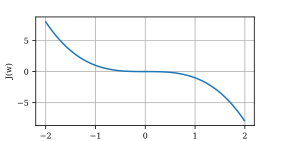
\includegraphics[scale=1]{Figures/Chapter_3/saddle_point.png}
	\end{center}
	\caption{Saddle point.} 
	\label{fig:saddle_point}
\end{figure}
%%%%%%%%%%%%%%%%%%%%%%%%%%%%%%%%%%%%%%%%%%%%%%%%%%%%%%%%%%%%%%%%%%%%%%%%%%%%%%%%
\subsection{Convolutional Neural Network} 
Convolutional Neural Networks (CNNs) are a special type of artificial neural network (ANN) that were initially developed in the 1980s by ~\textcite{Fukushima1980} who was inspired by the discoveries of Hubel and Wiesel regarding the cat's visual cortex. 
CNNs are one of the most utilised architectures in DL for image processing as they can recognise complex patterns of images by performing convolution operations.

In mathematics, a convolution is an operation performed between any two functions, as for example \(f, g:\mathbb{R}^{d} \to \mathbb{R}\) to produce at third function \((f\ast g)\) depicted in Eqn.~\ref{eqn:convolution}.
In which, we measure the overlap between \(f\) and \(g\), as one function is flipped and shifted by \(x\):
\begin{equation}
	(f\ast g)(x) = \int_{}^{} f(z)g(x-z)dz
	\label{eqn:convolution}
\end{equation}
In the case of discrete objects defined on the set \(\mathbb{Z}\) of integers, the integral operation turns into a summation of elementwise multiplied components, as depicted in Eqn.~\ref{eqn:discrete_conv}:
\begin{equation}		
	(f\ast g)(x) = \sum_{a}^{} f(a)g(i-a)
	\label{eqn:discrete_conv}
\end{equation}
For inputs with two dimensions, we have a corresponding sum with indices \((a,b)\) for \(f\) and \((i-a, j-b)\) for \(y\) respectively as depicted in Eqn.~\ref{eqn:2d_conv} that describes a cross correlation operation:
\begin{equation}
	(f\ast g)(i,j) = \sum_{a}^{}\sum_{b}^{}f(a,b)g(i-a,j-b)
	\label{eqn:2d_conv}
\end{equation}
%%%%%%%%%%%%%%%%%%%% from here
Convolution operation for image processing is essentially a cross-correlation operation also known as a sliding dot product or sliding inner-product. 
CNNs were designed to process data as tensors with different dimensions. 
For a 1D data tensor, it can represent various data forms, such as signals and sequences, in addition to sentences in various languages in translation problems.
For a 2D data tensor, it can represent an image in grayscale (one channel), further, by combining three 2D tensors a coloured 3D image is produced due to different intensities of the pixels in the (RGB) channels.
A 4D tensor represents volumetric data, such as a sequence of 3D images or a video.

A convolutional layer, has a number \( n\) of convolution kernels (filters), in  which,  each kernel has a set of weights, of a size \((w_k,h_k,d_k)\).
The kernel slides over an input image of a size \((w,h,d)\) performing a convolution operation (dot product), where \(w\) and \(h\) represent the image width and height, respectively, while \(d\) represents the depth (number of channels).
The output of the convolution operation are feature maps that are locally connected to the output of the previous layer. 
Figure~\ref{fig:convolution_3d} illustrates the convolution operation for a 3D input and the calculated output (feature map) with a new shape of \((h_{n}\times w_{n} \times d_{n})\).
%%%%%%%%%%%%%%%%%%%%%%%%%%%%%%%%%%%%%%%%%%%%%%%%%%%%%%%%%%%%%%%%%%%%%%%%%%%%%%%%
\begin{figure} [!ht]
	\begin{center}
		\centering
		\includegraphics[width=0.75\textwidth]{Figures/Chapter_3/convolution_operation_3D.png}
	\end{center}
	\caption{Convolution operation with a sliding kernel.} 
	\label{fig:convolution_3d}
\end{figure}
%%%%%%%%%%%%%%%%%%%%%%%%%%%%%%%%%%%%%%%%%%%%%%%%%%%%%%%%%%%%%%%%%%%%%%%%%%%%%%%%

Typically, the feature map size diminishes due to the convolution operation, though, the feature map can keep the same size of the input by applying some padding over the input. 
The calculations of new height and width of the output are illustrated in Eqns~\ref{new_hight} and~\ref{new_width}:
%%%%%%%%%%%%%%%%%%%%%%%%%%%%%%%%%%%%%%%%%%%%%%%%%%%%%%%%%%%%%%%%%%%%%%%%%%%%%%%
\begin{equation}
	h_{n} = \frac{h+2\times p-h_{k}}{s}+1
	\label{new_hight}
\end{equation}
%%%%%%%%%%%%%%%%%%%%%%%%%%%%%%%%%%%%%%%%%%%%%%%%%%%%%%%%%%%%%%%%%%%%%%%%%%%%%%%%
\begin{equation}
	w_{n} = \frac{w+2\times p-w_{k}}{s}+1.
	\label{new_width}
\end{equation} 
where \(h_{n}\) and \(w_{n}\) are the new height and width dimensions of the feature map respective\-ly after applying the convolution. 
The padding \(p\) is added to the input image of a feature map to guarantee that both the input and the output have the same dimensions.
\(h_{k}\) and \(w_{k}\) represent the height and the width of the convolutional kernel, respectively.
The stride \(s\) defines how much the convolutional kernel slides each step during convolution.
The number of channels at the output feature map \((d_{n})\) equals the applied number of convolutional kernels \((n)\). 

Typically,  when we train a CNN model, its kernel weights are initialised randomly.
Accordingly, during the backpropagation process, all learnable parameters (kernels weights) are updated.
Consequently, kernels learn to detect different types of edges (vertical, horizontal, and diagonal edges), color intensities, etc.
%%%%%%%%%%%%%%%%%%%%%%%%%%%%%%%%%%%%%%%%%%%%%%%%%%%%%%%%%%%%%%%%%%%%%%%%%%%%%%%%

Commonly, a convolutional operation is followed by a non-linear activation function such as (relu, sigmoid, tanh), followed by a downsampling operation (pooling).
The idea behind pooling operation is to aggregate related features into one by reducing the spatial dimensions of the feature maps (e.g., width, height, and depth)~\cite{Lecun2015}, which reduces the computation complexity.
Figure~\ref{fig:downsampling} presents the downsampling operations that are max and average pooling, further, the pool size is \(2 \times 2\) with strides of \(2\).
The Maxpool picks the maximum value in the local pool filter in a feature map, whereas the average pool picks the average value in the local pool filter in a feature map.
%%%%%%%%%%%%%%%%%%%%%%%%%%%%%%%%%%%%%%%%%%%%%%%%%%%%%%%%%%%%%%%%%%%%%%%%%%%%%%%%
\begin{figure} [!ht]
	\begin{center}
		\centering
		\includegraphics[scale=1]{Figures/Chapter_3/downsampling.png}
	\end{center}
	\caption{Types of downsampling operations.} 
	\label{fig:downsampling}
\end{figure}
%%%%%%%%%%%%%%%%%%%%%%%%%%%%%%%%%%%%%%%%%%%%%%%%%%%%%%%%%%%%%%%%%%%%%%%%%%%%%%%%
A convolution operation, followed by a non-linear activation function, and pooling is referred to as a convolutional block.
Moreover, a convolutional block can be stacked and repeated several times. 
Finally, to pass the output from the convolutional block to the dense layer, a flattened layer is utilised to produce a 1D tensor.
Figure~\ref{fig:CNN} presents the default architecture of a CNN.
%%%%%%%%%%%%%%%%%%%%%%%%%%%%%%%%%%%%%%%%%%%%%%%%%%%%%%%%%%%%%%%%%%%%%%%%%%%%%%%%
\begin{figure} [!ht]
	\begin{center}
		\centering
		\includegraphics[width=1\textwidth]{Figures/Chapter_3/cnn.png}
	\end{center}
	\caption{Convolutional Neural Network architecture.} 
	\label{fig:CNN}
\end{figure}
%%%%%%%%%%%%%%%%%%%%%%%%%%%%%%%%%%%%%%%%%%%%%%%%%%%%%%%%%%%%%%%%%%%%%%%%%%%%%%%%

CNN became popular after the competition of the \enquote{Large Scale Visual Recognition Challenge 2012 (ILSVRC2012)}, when \textcite{Krizhevsky2012} introduced AlexNet~\cite{Krizhevsky2012}, which is a deep CNN applied on a large dataset of \(1,000,000\) images and \(1,000\) different classes.
AlexNet results were magnificent. 
The success has stimulated the progress of the development in GPUs technology and the use of the non-linear activation function Relu~\cite{Lecun2015}.
In the next years, several spectacular CNNs architectures were presented (e.g VGG-16, ResNet, Inception-v4, and others).
%%%%%%%%%%%%%%%%%%%%%%%%%%%%%%%%%%%%%%%%%%%%%%%%%%%%%%%%%%%%%%%%%%%%%%%%%%%%%%%%
\subsection{Recurrent neural networks}
\label{sec222}
Recurrent neural network (RNN) is a class of ANN that was introduced to work with time-series data (sequential data).
RNN technique can remember its data input, because of its internal memory, which makes it a powerful and promising technique in the field of DL.
Since there are temporal problems such as natural language processing, language translation, image captioning, and so on, they require to be handled sequentia\-lly.
In the traditional deep neural networks (feed-forward), the information only moves in one direction from the input layer through hidden layers to the output layers.
However, this is not the case for the RNN technique, which implies the current output of an RNN depends on the prior input sequence.
Accordingly, future events are also utilised for predicting the output of a given sequence.
Figure~\ref{fig:rnn_vs_FFNN} depicts the difference between RNN and feed-forward deep neural networks.
As shown in Fig.~\ref{fig:rrn}, for the RNN, the output of a certain layer is looped back to its input which helps in making the prediction.
However, in feed-forward networks shown in Fig.~\ref{fig:FFNN}, the inputs and outputs are independent, as there is only one direction for the data to move.
%%%%%%%%%%%%%%%%%%%%%%%%%%%%%%%%%%%%%%%%%%%%%%%%%%%%%%%%%%%%%%%%%%%%%%%%%%%%%%%%
\begin{figure}[!ht]
	\centering
	\begin{subfigure}{0.49\textwidth}		
		\centering
		\includegraphics[scale=1]{Figures/Chapter_3/recurrent_NN.png}
		\caption{} 
		\label{fig:rrn}
	\end{subfigure}
	\hfill
	\begin{subfigure}{0.49\textwidth}
		\centering
		\includegraphics[scale=1]{Figures/Chapter_3/feedforward_NN.png}
		\caption{} 
		\label{fig:FFNN}
	\end{subfigure}	
	\caption{(a) RNN v.s. (b) Feed-forward neural network.}
	\label{fig:rnn_vs_FFNN}
\end{figure}
%%%%%%%%%%%%%%%%%%%%%%%%%%%%%%%%%%%%%%%%%%%%%%%%%%%%%%%%%%%%%%%%%%%%%%%%%%%%%%%%

Figure~\ref{unrolled_rnn} presents a visualisation of an unrolled RNN, where \(x_{t}\) corresponds to the sequential timestamped input at time \(t\), \(h_{t}\) corresponds to internal state  and \(Y_{t}\) corresponds to the predicted timestamped output at time \(t\).
An unrolled RNN can be seen as a cascaded sequence of feed-forward networks.
%%%%%%%%%%%%%%%%%%%%%%%%%%%%%%%%%%%%%%%%%%%%%%%%%%%%%%%%%%%%%%%%%%%%%%%%%%%%%%%%
\begin{figure}
	\begin{center}
	\includegraphics[scale=1]{Figures/Chapter_3/unrolled_rnn.png}
	\end{center}
	\captionof{figure}{Unrolled RNN.}
	\label{unrolled_rnn}
\end{figure}
%%%%%%%%%%%%%%%%%%%%%%%%%%%%%%%%%%%%%%%%%%%%%%%%%%%%%%%%%%%%%%%%%%%%%%%%%%%%%%%%

In feed-forward neural networks, the learnable parameters (adjustable weights) are available only for the forward path of data propagation and are updated through the back-propagation algorithm.
In RNNs, there are two paths of data propagation (forward and backward). 
Hence, there are learnable weights for both directions.
Further, weights are updated using back-propagation through time (BBTT)~\cite{Werbos1990}.
BBTT depends on the number of timestamps, so it is computationally expensive when there are a high number of timestamps as BBTT performs a back-propagation algorithm on unrolled RNN.
Consequently, when implementing RNNs, issues may arise during updating the learnable weights using BBTT, which are vanishing and exploding gradien\-ts.
To overcome such issues, ~\textcite{Hochreiter1997} introduced a long short-term memory (LSTM), which is a memory extension for a regular RNN to address the problem of long-term dependencies.
Further, LSTMs handle inputs or outputs of any length, which makes LSTMs powerful for solving very complex sequential problems.
LSTM is composed of four units: an input gate, a cell state, a forget gate, and an output gate as presented in Fig.~\ref{fig:lstm}.
These gates help regulate the flow of information, which is added to or removed from the cell state. 
The hidden states in LSTM hold the short-term memory, while the cells state holds the long-term memory.
%%%%%%%%%%%%%%%%%%%%%%%%%%%%%%%%%%%%%%%%%%%%%%%%%%%%%%%%%%%%%%%%%%%%%%%%%%%%%%%%
\begin{figure}[h!]
	\begin{center}
		\includegraphics[scale=1]{Figures/Chapter_3/lstm.png}
	\end{center}
	\captionof{figure}{LSTM architecture.}
	\label{fig:lstm}
\end{figure}
%%%%%%%%%%%%%%%%%%%%%%%%%%%%%%%%%%%%%%%%%%%%%%%%%%%%%%%%%%%%%%%%%%%%%%%%%%%%%%%%

The purpose of the forget gate is to determine which information to consider and which to neglect.
The current input \(x_t\) and the previous hidden state \(h_{t-1}\) are passed through a sigmoid function which will produce values between \(0\) and \(1\).
Then the outputs of the sigmoid are multiplied with the previous cell state \(c_{t-1}\) to discard outputs equal to zero.
Equation~\ref{eqn:forget_gate} depicts the calculation at the forget gate:
%%%%%%%%%%%%%%%%%%%%%%%%%%%%%%%%%%%%%%%%%%%%%%%%%%%%%%%%%%%%%%%%%%%%%%%%%%%%%%%%
\begin{equation}
	\centering
	f_t = \sigma(W_f.[h_{t-1}, X_{t}]+ b_f),
	\label{eqn:forget_gate}
\end{equation}
%%%%%%%%%%%%%%%%%%%%%%%%%%%%%%%%%%%%%%%%%%%%%%%%%%%%%%%%%%%%%%%%%%%%%%%%%%%%%%%
where \(W\) represents the learnable weights, and \(b\) represents the bias term.

The input gate \(i_{t}\) takes the current input \(X_t\) with the previous hidden state \(h_{t-1}\) then apply the sigmoid function to get values in a range between 0 (not important) and 1 (important), then the
same current input \(X_t\), and the hidden state \(h_{t-1}\) are passed through a \(\tanh\) function at \(\tilde{C}_{t}\) that will regulate the network by transferring the values into a range between \(-1\) and \(1\).
Then, the outputs from the sigmoid and \(\tanh\) functions are multiplied point-by-point to eliminate \(0\) values.  
Equation~\ref{eq:eq2} depicts the calculation at the input gate:
\begin{equation}
	\begin{aligned}
		i_{t} &=\sigma\left(W_{i} \cdot\left[h_{t-1}, X_{t}\right]+b_{i}\right) ,
		\\
		\tilde{C}_{t} &=\tanh \left(W_{s} \cdot\left[h_{t-1}, X_{t}\right]+b_{c}\right).
	\end{aligned} \label{eq:eq2}
\end{equation}
At this point, the network has sufficient information obtained from the input and forget gates. 
Hence, the current cell state \(C_t\) is calculated by multiplying the previous cell state \(C_{t-1}\) with the output of the forget gate, then the result is added to the calculated input values as depicted in Eqn.~\ref{eq:eq3}:
\begin{equation}
	C_{t}=f_{t} * C_{t-1}+i_{t} * \tilde{C}_{t}.
	\label{eq:eq3}
\end{equation}
The output gate \(o_{t}\) computes the next hidden state \(h_{t}\) which
holds information related to the current inputs. 
Accordingly, the current input \(X_{t}\) and the previous hidden state \(h_{t-1}\) are passed through a third sigmoid function to produce values between \(0\) and \(1\).
The current cell state \(C_{t}\) is passed through a \(\tanh\) function and multiplied point-by-point with \(o_{t}\) to produce the new hidden state \(h_{t}\) which is transferred to the next timestamp.
Equation~(\ref{eq:eq4}) illustrates the calculations at the output gate:
%%%%%%%%%%%%%%%%%%%%%%%%%%%%%%%%%%%%%%%%%%%%%%%%%%%%%%%%%%%%%%%%%%%%%%%%%%%%%%%%
\begin{equation}
	\begin{aligned}
		o_{t} &=\sigma\left(W_{o}\left[h_{t-1}, X_{t}\right]+b_{o}\right),\\
		h_{t} &=o_{t} * \tanh \left(C_{t}\right).
	\end{aligned}
	\label{eq:eq4}
\end{equation} 
%%%%%%%%%%%%%%%%%%%%%%%%%%%%%%%%%%%%%%%%%%%%%%%%%%%%%%%%%%%%%%%%%%%%%%%%%%%%%%%%

Recently, LSTMs have been widely used for large-scale learning of language translation models, speech recognition systems, chatbots, forecasting stock markets, text data analysis, and many more~\cite{graves2014towards, cho2014properties}.
However, LSTMs are inefficient regarding capturing spatial information by themselves when the time series inputs are consecutive images.
Accordingly, the ConvLSTM layer, which is a combination of CNN and LSTM unit was introduced by Shi et al.~\cite{xingjian2015convolutional} to solve such a problem.
For ConvLSTM, the convolution operations are applied both at the input-to-state transition and at the state-to-state transitions.
ConvLSTM shown in Fig.~\ref{fig:ConvLSTM} is a variation of the LSTM cell as it performs a convolution operation within the LSTM cell.
%%%%%%%%%%%%%%%%%%%%%%%%%%%%%%%%%%%%%%%%%%%%%%%%%%%%%%%%%%%%%%%%%%%%%%%%%%%%%%%%
\begin{figure}[h!]
	\begin{center}
		\includegraphics[scale=1]{Figures/Chapter_3/convlstm_image.png}
	\end{center}
	\captionof{figure}{ConvLSTM architecture.}
	\label{fig:ConvLSTM}
\end{figure}
%%%%%%%%%%%%%%%%%%%%%%%%%%%%%%%%%%%%%%%%%%%%%%%%%%%%%%%%%%%%%%%%%%%%%%%%%%%%%%%%
ConvLSTM is a combination of a convolution operation and an LSTM cell.
Thus, ConvLSTM can capture the time-correlated and spatial features in a series of consecutive images. 
Equation~(\ref{eq:eq5}) depicts the ConvLSTM operations as the inputs \(X_1, \dots, X_t\), hidden states \(h_1, \dots, h_t\), cell states \(C_1, \dots, C_t\) and input, forget and output gates are represented as \(i_t, f_t\), and \(o_t\), respectively:
\begin{equation}
	\begin{aligned}
		i_{t} &=\sigma\left(W_{x i} * X_{t}+W_{h i} * h_{t-1}+W_{c i} \odot C_{t-1}+b_{i}\right) 
		\\
		f_{t} &=\sigma\left(W_{x f} * X_{t}+W_{h f} * h_{t-1}+W_{c f} \odot C_{t-1}+b_{f}\right) \\
		C_{t} &=f_{t} \odot C_{t-1}+i_{t} \odot \tanh \left(W_{x c} * X_{t}+W_{h c} * h_{t-1}+b_{c}\right) 
		\\
		o_{t} &=\sigma\left(W_{x o} * X_{t}+W_{h o} * h_{t-1}+W_{c o} \odot C_{t}+b_{o}\right) \\
		h_{t} &=o_{t} \odot \tanh \left(C_{t}\right)
	\end{aligned}
	\label{eq:eq5}
\end{equation}
where \(*\) indicates the convolution operation, and \(\odot\) represents the 
Hadamard product. 
Recently, ConvLSTM has become very popular and is increasingly being used in 
more and more image processing applications.
\section{Data-driven based SHM/NDT Techniques: Related work}
\label{sec33}
%%%%%%%%%%%%%%%%%%%%%%%%%%%%%%%%%%%%%%%%%%%%%%%%%%%%%%%%%%%%%%%%%%%%%%%%%%%%%%%%
The importance of SHM systems originated from their ability to monitor the condition of structures in real-time.
SHM systems can be developed using data-driven methods, which require a huge amount of data that are captured by monitoring the status of a structure.

The process of extracting features from structures in conventional techniques needs a lot of time and experts in the field. 
Therefore, introducing machine learning methods to the feature extraction process became necessary.
Hence, deep learning methods have the capability to generalise and learn new features by themselves, which improves their functionality in damage estimation.

DL approach makes it possible to use registered data in their raw form without any need to perform feature extraction.
Hence, such an approach has an end-to-end structure that automatically learns and discovers the hidden features in a high dimensional input data~\cite{LeCun, Networks}.
Figure~\ref{fig:ML_vs_DL} illustrates the main differences between the conventional ML-based SHM and DL-based SHM approaches.

\begin{figure}[!ht]
	\centering
	\begin{subfigure}{1\textwidth}		
		\centering
		\includegraphics[width=1\textwidth]{Figures/Chapter_3/conventional_ML.png}
		\caption{} 
		\label{fig:ML_conventional}
	\end{subfigure}
	\\
	\begin{subfigure}{1\textwidth}
		\centering
		\includegraphics[width=1\textwidth]{Figures/Chapter_3/DL_approach.png}
		\caption{} 
		\label{fig:DL_approach}
	\end{subfigure}	
	\caption{(a) Conventional ML based SHM vs. (b) DL based SHM.}
	\label{fig:ML_vs_DL}
\end{figure}
%%%%%%%%%%%%%%%%%%%%%%%%%%%%%%%%%%%%%%%%%%%%%%%%%%%%%%%%%%%%%%%%%%%%%%%%%%%%%%%%
\textcite{Worden2007} have proposed several axioms related to SHM systems implemented using machine learning methods. 
According to them, damage detection can be perform\-ed in unsupervised learning.
However, recognising the damage type and how significant it is can not be performed without supervised learning. 
Moreover, the feature extraction process is essential for damage detection, and it can be performed through analysing and processing the signals captured by the sensors (e.g. PZT actuators), then converting them to damage information.
Therefore, introducing machine learning methods to the feature extraction process became necessary.
Hence, machine learning methods have the capability to generalise and learn new features by themselves, which improves their functionality in damage estimation.

\subsection{Machine leaning based SHM/NDT}
In recent years data-driven methods based on machine learning have been increased in a significant way. 
In the following, I will present some methods for damage detection and estimation based on machine learning techniques.

%%%%%%%%%%%%%%%%%%%%%%%%%%%%PZT + SVM
\textcite{Das2010} presented a method for estimating several types of defects (delamination, saw cut, notches, and drilled holes) in composite material. 
For this purpose, a collection of PZT transducers were attached to the surface of the structure to generate and register Lamb waves propagation. 
Accordingly, a time-frequency domain was utilised to extract features related to defects from the registered response. 
Those extracted features were fed to one-class SVM, which performs classification and damage estimation. 
%%%%%%%%%%%%%%%%%%%%%%%%%%%% PZT + SVM
Moreover, \textcite{Dib2018} proposed a novelty classifier based on one-class SVM for detecting damage. 
The method was conducted by extracting data from damage impact on a glass-fibre composite plate, then evaluating the performance of the classifier. 
To extract the necessary features from the propagated wave the registered signal was segmented into L time bins, and the Fourier transform was applied on each time bin.
Accordingly, the features vector was constructed from the signal phase and the amplitude for each segmented time bin.

%%%%%%%%%%%%%%%%%%%%%%%%%%%%%%%%% PZT + PCA+ KNN + SVM
\textcite{Vitola2016} developed a damage detection and classification methodology that was examined on aluminium plates.
An array of PZT transducers was placed on the plate surface to sense wave propagation in the structure.
The methodology is based on the use of principal component analysis (PCA) and machine learning techniques for recognising patterns. 
PCA means to analyse a large amount of information by finding the principal components.
However, the PCA method is not invariant to scaling, thus, data must be normalized~\cite{Tibaduiza2016}. 
Next, normalised data is fed to several machine learning models for training. 
For this purpose, several classification algorithms were applied, decision trees, KNN and SVM. 
However, only a few of these models presented good outputs in damage detection. 

%%%%%%%%%%%%%%%%%%%%%%%%%%% KNN
\textcite{Godin2004} applied Acoustic Emission signals (AE) in their approach, which happen due to a sudden release of stored energy when damage occurs.
AE signals contain important information about the discriminative features 
for the damage type such as fibre breakage, de-cohesion of the interface, or a crack in the matrix in composite materials.
Authors in this work presented supervised and unsupervised classifiers to recognise different damage patterns through grouping AE signals from the tensile tests of unidirectional glass/polyester composite into several different classes. 
For clustering AE signals, a K-means algorithm was used. 
AE signals were clustered based on several metrics such as the AE signal duration, amplitude, rise time, and the number of counts to the peak.
Accordingly, the clustered labelled data is fed into a KNN supervised classifier.
A trained classifier is able to classify new coming data accordingly.
Regarding the unsupervised classification, the Kohonen classifier was utilised~\cite{58325}, which is a self-organising map (SOM) which is a neural network consisting of neurons as processing units. 
%%%%%%%%%%%%%%%%%%%%%%%%%%% 

\textcite{Nazarko2020} monitored the axial bolt forces using elastic wave propagation signals.
Six-bolt flange connections were put through a series of static tensile tests in the lab. For the accurate measurement of axial force, some bolts were equipped with washer load cells.
Additionally, a few bolts were equipped with piezoelectric transducers (actuator and sensor operating in a pitch-catch arrangement) to capture the elastic wave signals.
The outcomes of the ultrasonic testing were then integrated with the artificial neural network (ANN) for both signal compression and as a tool for user interface. 
The outcomes demonstrated that ANNs could predict the axial forces in bolts with a reasonable amount of accuracy. 
Significant potential exists for actual NDT inspections, according to the suggested method~\cite{Nazarko2020}. 

%%%%%%%%%%%%%%%%%%%%%%%%%%% KNN
\textcite{Pashmforoush2014} proposed a technique to classify damage of various lay-up configurations in glass/polyester composites.
For this purpose, the K-means algorithm with the genetic algorithm was utilised. 
PCA was used to reduce the data dimensionality.
Next, a combination of the K-means algorithm with the genetic algorithm is used for clustering the data. 
The reason for applying the genetic algorithm is to find the optimal number of cluster centres for the KNN algorithm.
Parameters of the AE signals such as peak amplitude, frequency, rise time, energy, and duration were estimated for each cluster and utilised as discriminative features. 
AE signal frequency was found to be a good feature for discrimination. Accordingly, AE signals with the highest frequency were corresponding to fibre breakage, AE signals with the lowest frequency were corresponding to matrix cracking, and the frequencies range in-between were corresponding to the debonding defect. 

%%%%%%%%%%%%%%%%%%%%%%%%%%%%%%%%%%%%%%%%%%%%%%%%%%%%%%%%%%%%%%%%
\textcite{Nazarko2016} investigated the potential of utilising artificially deteriorated signals of Lamb waves in training a novelty detection (ND) system for early damage detection.
In order to train auto-associative neural networks, the authors used principal components that were generated from signals that were measured experimentally.
The measurements of Lamb waves in the investigated specimens made of aluminum and glass fiber reinforced polymer serve as an excellent illustration of how the ND algorithm accurately handles both simple and complex signals.
It was also noted that the proposed ND method maintained its sensitivity and robustness when it used raw signals with a relatively low sampling rate, on a relatively narrow time window, and further noised signals.
%%%%%%%%%%%%%%%%%%%%%%%%%%%% PZT + ConvNet
%\textcite{Sammons2016} utilised X-ray computed tomography for estimating the delaminations in a CFRP. For this purpose, they utilised the Convolutional Network (ConvNet ) for performing image segmentation of the defected input images to estimate the delaminations. There ConvNet was capable of identifying  and quantifying small delaminations. 
%Unfortunately, the ConvNet could not recognise delaminations with large sizes.
%%%%%%%%%%%%%%%%%%%%%%%%%%%% PZT + ConvNet
%
%Moreover, \textcite{Chetwynd2008} have investigated curved carbon fibre composite panel for damage localisation. 
%Accordingly, stiffeners were used during the experiments to represent real-life damage. 
%For this purpose, authors attached a combination of PZT transducers on the panel used to generate and receive Lamb waves that propagate through the structure. 
%During their propagation through the structure, Lamb waves encounter defects, which affects their propagation response. 
%The collected response was transformed into a novel scaler index using outlier analysis~\cite{Beniger1980}, which was then fed to MLP. 
%The MLP used for classification and regression applications of damage detection. 
%Classification operation is responsible for predicting whether there is damage or not in a specific location. 
%Where the regression operation is responsible for the exact estimation of the damage location.
%%%%%%%%%%%%%%%%%%%%%%%%%%% Ful wavefield +ConvNets
%% SECTION HEADER ////////////////////////////////////////////////////////////////////////////////
\subsection{Deep learning based SHM/NDT}

Deep learning techniques have widely been utilised for the inspection and maintenance of civil infrastructure and have shown very promising results \cite{Cha2017b, Lin2017, liu2019computer, Beckman2019, Choi2020, Sonski2020a, Sonski2020, Sonski2019}. 

Besides the widespread applications of deep learning for SHM/NDT in civil engineering, deep learning is still less investigated for the purpose of damage detection based on guided waves in composite materials.

Guided waves approaches are widely utilised in SHM/NDT due to the fact it can detect very small damage sizes~\cite{Guemes2020}. 
Damage detection and localisation approaches using guided waves are based on the measurements of the PZT sensors, whether bonded or embedded into the investigated structure. 
PZT sensor(s) are responsible for the excitation of the structure by a short ultrasonic pulse (usually, the used frequency is in the range of hundreds of kHz) that propagates through an investigated structure such as plates or pipes as an elastic wave.
The registered signals (baseline) are stored and compared with other registered signals acquired through the lifetime of the investigated structure.
Damage detection using the baseline subtraction approach for guided waves is based on subtracting damage-free registered measurements from the newly registered measurements to obtain the new changes that occurred to the structure.
These changes are considered as damage information.
The baseline approach is effective in controlled environments where the variations of the operational/environments (i.e. considerations of multiple sensing modalities, uncertainty in material properties, bounding conditions, etc.) are negligible~\cite{Yuan2020}.  
Such variations can alter registered data leading to false alarms.
The effect of such variations can be reduced through physics-based modeling, which can simulate an undamaged scenario (baseline) for the wave propagation through the investigated structure.
Then, the simulated baseline can be used in the subtraction for damage detection.
However, in real-world structures, it is difficult to adjust the parameters of the model to match the experimental registered data.
Accordingly, data-driven techniques based on ML and DL approaches can be the solution and deliver robust models for many real-life variations.

In the following, methods for damage size estimation based on machine learning and deep learning techniques are presented, which are targeted in the field of SHM/NDT.

%\textcite{islam1994damage} presented one of the earliest research studies for assessing delamination location and size in composite structures using deep learning techniques.
%They trained a neural network model using frequencies from modal analysis data for the first five modes.
%Data were obtained using piezoceramic sensors in both damaged and undamaged composite beams.
%In the following, several approaches utilising guided waves for SHM/NDT based on data-driven techniques for damage detection and localisation are presented.

\textcite{Melville1949} proposed a CNN model for the prediction of damage state in thin metal plates to overcome the issue of inaccurate representation of guided wave propagation when applying conventional approaches. 
The model utilizes the full wavefie\-ld scans of thin plates (aluminum).
Moreover, the acquired raw data used for training the model was divided into undamaged and damaged states equally.
The model achieved higher accuracy regarding damage detection equal \(99.98\%\) when compared to SVM that achieved \(62\%\).

\textcite{Sammons2016} proposed a CNN model based on X-ray computed tomography for delamination estimation in a composite structure.
Furthermore, image segmentation was applied to the input images to identify the damage.
However, the model was only able to identify small delaminations.

Moreover,~\textcite{Chetwynd2008} presented a multi-layer perceptron (MLP) network for damage detection in curved composite panels, in which, stiffeners were added to represent the damage.
The Authors in this work investigated the propagation of Lamb waves through the panel in which they were generated and registered by a PZT array.
Furthermore, for each Lamb wave response, a novelty index was obtained.
The index value is compared to some threshold value, in which if the index value exceeds the threshold it implies that there is damage in the structure.
Accordingly, the MLP network was fed by obtained novelty indexes, and performed two operations: classification and regression.
The classification network was designed to define three convex regions of the panel then to determine whether the panel is damaged or not.
On the other hand, the regression network is capable of estimating the exact location of the damage.

Furthermore,~\textcite{DeFenza2015} proposed an artificial neural network (ANN) model for damage detection in plates made of aluminum alloys and composite utilising Lamb waves.
Response data of wave propagation were used to calculate damage indexes which were fed into the model as an input.
Accordingly, the model performs automatic feature extraction in conjunction with the probability ellipse-based method. 
The ANN model and probability ellipse (PE) method were applied to identify damage location.
The results from the ANN model and the PE presents how it is useful to apply damage indexes as a baseline for such methods in order to evaluate damage in aluminum and composite structures. 
Ewald et al.~\cite{Ewald2019} presented a CNN model called (DeepSHM) for signal classification using Lamb waves.
Furthermore, the model provides an end-to-end approach for SHM by utilising response signals captured by sensors.
Moreover, response signals were preprocessed by wavelet transform to get the wavelet coefficient matrix (WCM).
Further, the CNN model was trained with the WCM to obtain neural weights.

Full wavefield scanning using SLDV is time-consuming, however, simply reducing the number of scanning points will result in low-quality images. 
\textcite{esfandabadideep} proposed a compressive Sensing technique using ConvNets to enhance the resolution for images captured by SLDV while decreasing the number of measurement scan points down to \(10\%\) of the number of the full gird scanning points. 
Although, the proposed technique enhanced the image resolution, however, there is a side effect, which resembles the fact when enhancing the resolution, the most affected region is the damaged area. 
Accordingly, the damage features will be altered.
On the other hand, this may be an indication to the location of the damage.

Furthermore,~\textcite{Melville2018} proposed a technique for damage detection in thin metal plates (aluminum and steel), using full wavefield data scanned by SLDV. 
Using this data to train a deep neural network of 4 hidden layers including 2 convolutional layers for features extraction and 2 fully connected layers. 
The developed model shown good results when compared with traditional machine learning SVM.
Moreover,~\textcite{Melville2017} introduced a method for detecting damage in structures based on the k-means algorithm. 
The method is known as~\enquote{dictionary learning} which uses full wavefield data collected from thin metal plates. 
The method was applied to structures with different material types and thicknesses that were not used during training to prove how well the model in damage detection in various conditions. 
However, their work was not implemented for a further step, which is damage localization and classification.

%\textcite{Ijjeh2021} presented a fully convolutional network (FCN)  for damage identification in composite plates base on a supervised learning approach.
%Furthermore, the authors utilised a full wavefield of Lamb waves propagation, which was numerically generated resembling measurements acquired by scanning laser Doppler vibrometer (SLDV).
%The model performs a pixel-wise segmentation that is able to identify the delamination which results in damaged and undamaged classes.
%Moreover, the model results were validated through a comparison with a conventional wavefield signal processing method i.e. adaptive wavenumber filtering~\cite{Radzienski2019,Kudela2018}.
%The proposed model achieved an accuracy of \(93.3\%\) in damage detection on numerical data compared to  \(64.8\%\) with the conventional method.
%Furthermore, the proposed model was verified on experimental data and it proved its ability for generalisation.
%%%%%%%%%%%%%%%%%%%%%%%%%%%%%%%%%%%%%%%%%%%%%%%%%%%%%%%%%%%%%%%%%%%%%%%%%%%%%%%%%%%%%%%%%%%%%%%%%%%%%%%%%%%%%%%%%%%%%%%%%%%%%%%%%%%%%%%%%%%%%%%%%%%%%%%%%%%%%%%%
%\subsection{Vibration based SHM though DL}
%\label{sec24}
%The vibration-based approach for damage assessment using ML techniques has been investigated thoroughly  for several SHM applications.
%Furthermore, introducing DL techniques for data-driven SHM applications has presented new scopes for investigating large scale structures and enhanced the process of data acquisition and processing of large datasets acquired by sensors of different types~\cite{Carden2004,Sohn1996}.
%Generally, the conventional approach for damage localisation requires prior knowledge of the approximate damage locations~\cite{Xu2018,Dorafshan2016}. 
%Therefore, the identification process regarding candidates for the damaged locations is complex and can consume plenty of time.
%Damage locations identification under the vibrational approach is based on the fact that the damage cause changes in the vibration characteristics such as modal shapes, frequencies, and damping~\cite{Doebling1998},
%which can be utilised in the identification of damaged locations from the registered data response of a structure.
%A vibration-based approach can be categorised into two classes:
%model-based (parametric) and non-model-based or (non-parametric).
%Parametric methods require computational models and associated assumptions about the investigated structure.
%In general parametric methods can achieve good accuracy, however, there is no guarantee regarding the availability of accurate information about the structural system in the real-world~\cite{Azimi2020}. 
%As a result, the non-parametric methods arise due to the challenges in developing robust computational models. 
%With non-parametric methods, there are no prior assumptions about the structural system.
%
%In the following, several vibration-based for SHM using DL techniques are presented.
%Authors in~\cite{Abdeljaber2017} introduced a damage identification approach based on output-only response data.
%In which, various damage cases (loose bolt) were investigated, accordingly training data were generated based on the acceleration response.
%Authors in this approach have trained several CNNs separately regarding each damage case, and accordingly, the probability of damage (PoD) was determined.
%By investigating scenarios of undamaged, single damage and multiple damage cases, they obtained \(0.54\%\) average error for specifically identified cases.
%
%Authors in~\cite{Lin2017} introduced a new approach to structural damage detection using CNN.
%Moreover, the authors have developed a numerical model of simply supported Euler Bernoulli beam.
%The detection model was designed to learn features and to identify damaged locations, moreover, it led to excellent results regarding the accuracy of damaged locations on the noise-free and noisy dataset.
%Wang and Cha in~\cite{Cha2018} proposed an unsupervised CNN model, that is able to extract the feature representations from the unlabelled data.
%The authors in their model used raw acceleration signals (sensitive to the damage presence) that were acquired from an intact lab-scale steel bridge.
%Then, the acquired response vector was normalised followed by applying the continuous wavelet transform (CWT) and fast Fourier transform (FFT).
%The output was then fed into a CNN auto-encoder,
%Accordingly, the extracted damage features were fed into one-class (OC) SVMs as novelty detectors corresponding to the sensors.
%Consequently, the approximation of damage location (loose-bolt) was estimated based on the locations of the sensors with the highest novelty rates.
%
%Motivated by human vision and thinking, authors in~\cite{Cha2018} presented a computer vision and deep-learning framework for anomaly detection.
%The proposed approach consists of two steps.
%In the first step, data conversion by data visualisation is carried out, in which it mimics human vision and thinking.
%In data visualisation,  the registered data response of acceleration is transformed into images plotted in gray-scale. 
%In the second step, the training dataset is labeled manually, then fed into deep convolutional neural networks (DCNNs).
%The proposed technique was tested on one-year data and achieved a global accuracy of \(87,0\%\) and it could be used for real-time SHM.
%Moreover, Tang et al. in~\cite{Tang2019} presented a DL technique for data anomaly detection which can be considered as an improved technique to the previous work in~\cite{Cha2018}.
%Initially, the raw time series measured data are split into segments, and data in the time and frequency domain are visualised. 
%Images related to each section are stacked as a single dual-channel (red and green).
%Then, the training dataset is fed into a CNN that learns how to perform data anomaly classification.
%The main difference between the previous approach and this approach was in using imbalanced data in which the number of samples of different classes was unequal, however, in this approach the used data were balanced.
%Finally, the comparison shows that this approach outperformed the previous one and achieved higher accuracy for all data anomaly patterns.
%
%Authors in~\cite{Wu2019} presented a study of the deep CNN method in estimating the dynamic response of a linear single-degree-of-freedom (SDOF) system, a nonlinear SDOF, and a multidegree of freedom (MDOF) streel frame.
%In some cases, the convolutional kernel can approximate the numerical integration operator, and the convolutional layer can be interpreted as a dominant frequency extraction operator.
%Moreover, different cases of noise-contaminated signals were investigated. 
%Additionally, MLP method was used as a reference to the proposed CNN approach.
%A comparison between the results obtained by the MLP and CNN shows that the CNN approach is more accurate and robust against noisy input data.
%
%Authors in ~\cite{Oh2019}  presented a study of the CNN technique for SHM application for response estimation of tall buildings under wind excitation.
%The proposed CNN model was trained on measured structural response data which take wind data measured as inputs in order to predict strains in future wind loads.
%In order to measure the performance of the proposed technique, it was verified with unseen data never used at the training phase and it was able to accurately estimate the maximum and minimum strains.
%Authors in~\cite{Li2020} proposed a CNN model for damage detection of a bridge structure.
%Moreover, the authors compared the performance of the CNN model with other techniques such as random forest, SVM, KNN, and decision tree, and the results showed that the accuracy was enhanced by at least \(15\%\).
%
%Since the acceleration response signal is highly prone to noise~\cite{Azimi2020}, researchers begin utilising other types of sensor data or use alternative features.  
%Li et al. in ~\cite{Li2020a} investigated damage in bridge structure accordingly, proposed a supervised learning technique based on the CNN model.
%Dataset was acquired by deflection of a scaled-down model bridge by a fibre-optic gyroscope.
%Then, the dataset was fed into a 1D-CNN model to classify three states of damage and an intact class (benchmark/damage-free).
%To investigate the performance of the proposed model, a cross-validation technique was applied. 
%It showed that the accuracy of the CNN model increased by at least \(15.3\%\) over other conventional methods such as SVM, KNN, decision trees, and random forests.
%Authors in \cite{Lopez-Pacheco2020} introduced a novel frequency-domain convolutional neural network (FDCNN) for damage detection based on Bouc-Wen hysteric model~\cite{Ismail2009}.  
%In the FDCNN method utilises only acceleration measurements for damage diagnosis, that are sensitive to environmental noise.
%Moreover, FDCNN reduces the computational time during the learning process, which increase noise robustness.
%The FDCNN introduced the spectral pooling operator responsible for attenuating the noise in measurements.
%The proposed method was validated through comparing it with different CNN model. 
%The performance of the proposed method was higher regarding damage identification in building structures.
%
%Finally, with smart monitoring as a target, authors in~\cite{Hung2020}  proposed a hybrid deep learning model for damage detection for SHM.
%The proposed model can deal with different damage levels and accurately detect damage by combining 1D-CNN and Long-Short Term Memory (LSTM) into a single end-to-end model fed by the raw time-series, and as a result, avoiding signal preprocessing step.
%Moreover, the proposed model verified that with low noise levels,  accurate damage detection can be achieved.
\section{Summary}
\label{sec34}
In this chapter, I presented several techniques that had studied and examined guided Lamb waves in composite materials to detect and localise the damage using signal processing techniques. 
Consequently, it can be concluded that DL methods have more and more applications in SHM/NDT in recent years. 
However, these are theoretical implementation rather than practical implementation in the field which can evidence of the lack of maturity of these methods. 
The other conclusion can be that it is observed that signal processing methods based on handcrafted feature extraction have been progressed into end-to-end approaches.
%those traditional techniques are complex and involve a huge numerical analysis and signal processing. Which concluded that the damage features are difficult to be extracted manually. 
%Thus, new approaches that involve Machine and Deep Learning techniques are utilised are presented in this chapter.
 
%As a result, the process of damage feature extraction became more convenient and easier since the machine is responsible for learning the new features and accordingly  detect and localise the damage. 
%In consequence, it is concluded that the advantage of this approach is the improvement of the procedure for damage feature extraction.
%
%Furthermore, problems with conventional damage detection techniques for SHM and the importance of the artificial intelligence approach were discussed.
%Furthermore, in the second section of the chapter, I introduced the ML approach in the SHM field.
%Moreover, several techniques for feature extraction such as PCA, MSD, and GMMs were described. 
%
%Further, several classification models such as SVM, KNN, and decision trees were introduced.
%Moreover, DL approach was introduced, in which techniques such as CNN  and RNN were presented.
%Finally, several deep learning techniques for damage detection used regarding the SHM field based on guided waves and vibration approaches were presented.
%\input{Chapters/Chapter3/sect35}
%\input{Chapters/Chapter3/sect36}
	%% CHAPTER HEADER /////////////////////////////////////////////////////////////////////////////////////
\chapter[Methodology]{Methodology}
\label{ch4}

%% CHAPTER INTRODUCTION ///////////////////////////////////////////////////////////////////////////////
In this chapter, I investigate several deep learning methodologies to detect and localise delamination in composite laminates.
The deep learning models were trained using a supervised scheme. 
Hence, it uses a training set to train the developed models to predict the desired output.
Accordingly, a synthetic dataset was built, representing the full wavefield of the Lamp waves propagating in a CFRP plate and their interaction with the delamination and the boundaries of the plate.
The acquisition process of the synthetic dataset is explained in details in the section~\ref{sec41}.

The developed methods are end-to-end approaches, in which the whole unprocessed training dataset is fed into the model.
Hence, it will learn by itself to identify distinct patterns and detect damage.
In section~\ref{sec42}, a fully connected CNN classifier model for detecting and localising delamination is presented in details.
In section~\ref{sec43}, I present five FCN models for delamination identification. Further, the developed models were trained using the RMS images in which the developed models are performing image pixel-wise image segmentation.
In section~\ref{sec44}, a deep learning model for delamination identification utilising the animation of full wavefield is presented.
Finally, in section~\ref{sec45}, I present a deep learning model for super-resolution image reconstruction.
Hence, the full wavefield of Lamb waves is recovered from low-resolution measurements into high-resolution measurements.
Accordingly, this can allow for a precise recovery of propagating waves and their interactions with delaminations and the boundaries of the plate.
Consequently, the reconstructed full wavefield can be used in damage imaging. 


All developed models were implemented and trained with the Keras API~\cite{chollet2015keras} running on top of TensorFlow~\cite{Abadi2016}.
The NVIDIA GeForce RTX 2070 with \(8\) GBs of memory was utilised to train the CNN classification models.
Furthermore, the NVIDIA Tesla V100 GPU with \(32\) GBs of memory was utilised to train the FCN models, the AE-ConvLSTM model, and the DLSR model.
%% INCLUDE SECTIONS ///////////////////////////////////////////////////////////////////////////////////

%% SECTION HEADER /////////////////////////////////////////////////////////////////////////////////////
\section{Synthetic data acquisition}
\label{sec41}
%%%%%%%%%%%%%%%%%%%%%%%%%%%%%%%%%%%%%%%%%%%%%%%%%%%%%
The crucial part in our work was in synthetically generating a dataset of a full wavefield of propagating of Lamb waves in a plate made of CFRP.
In which we
In this work, we have generated a large dataset of \(475\) cases of a full wavefield of propagating Lamb waves in a plate made of carbon fibre-reinforced plastic (CFRP).
The in-house code of the time-domain spectral element method was used for simulation of Lamb wave interaction with delamination~\cite{Kudela2020}.
It should be added that despite the utilisation of the parallel code of the spectral element method which was run on the Tesla K20X GPU card, the computation of the dataset (consisting of 475 cases) took about 3 months.
For each case, single delamination was modelled by using the method of splitting nodes between appropriate spectral elements. 
It was assumed that the composite laminate is made of eight layers of a total thickness of 3.9 mm.
The delamination was modelled between the third and fourth layer (see Fig.~\ref{fig:plate_setup} for details).
It should be noted that Fig.~\ref{fig:plate_setup} shows an exaggerated cross-section through the delamination. 
Zero-volume delamination was assumed in the model. 
Delamination spatial location was selected randomly so that the interaction of guided waves with delamination is different for each case.
It includes cases when delamination is located at the edge of the plate which is the most difficult to identify by signal processing methods.
Additionally, the size of the delamination of elliptic shape was randomly simulated by selecting the size of ellipse minor and major axis.
Also, the angle between the delamination major axis and the horizontal axis was randomly selected.
In summary the following random factors were simulated in each case:
\begin{itemize}
	\item delamination geometrical size	(ellipse minor and major axis randomly selected from the interval \(\left[10 \, \textrm{mm}, 40\, \textrm{mm}\right]\)),
	\item delamination angle (randomly selected from the interval \( \left[ 0^{\circ}, 180^{\circ} \right]\)),
	\item coordinates of the centre of delamination (randomly selected from the interval \(\left[0\, \textrm{mm}, 250\, \textrm{mm} -\delta \right]\) and \( \left[250\, \textrm{mm}+\delta, 500\, \textrm{mm} \right] \), where \(\delta = 10\, \textrm{mm}\)).
\end{itemize}
It resulted in random spatial placement of delaminations. The plate with overlayed 475 delamination cases is shown in Fig.~\ref{fig:random_delam}.
\begin{figure}
	\centering
	\includegraphics[scale=0.8]{Figures/Chapter_3/plate_delam_arrangement_MSSP.PNG}
	\caption{Setup for computing Lamb wave interactions with delamination.}
	\label{fig:plate_setup}
\end{figure}	
\begin{figure}
	\centering
	\includegraphics[scale=1]{Figures/Chapter_3/dataset2_labels_ellipses.png}
	\caption{The plate with 475 cases of random delaminations.}
	\label{fig:random_delam}
\end{figure}

Guided waves were excited at the plate centre by applying equivalent piezoelectric forces.
The excitation signal had a form of sinusoid modulated by Hann window. 
It was assumed that the carrier frequency is 50 kHz and the modulation frequency is 10 kHz.
A relatively low carrier frequency allowed for lower mesh density and significant computation time reduction in comparison to simulations of higher frequencies.
Additionally, the excitation signal was selected so that interaction of generated A0 Lamb wave mode with the smallest delamination can be still used as a feature for damage identification.

The output from the top and bottom surfaces of the plate in the form of particle velocities at the nodes of spectral elements were interpolated on the uniform grid of 500\(\times\)500 points by using shape functions of elements (see~\cite{Kudela2020} for more details).
It essentially resembles measurements acquired by SLDV in the transverse direction (perpendicular to the plate surface).
An example of the simulated full wavefield data on the top and bottom surfaces is presented in Fig.~\ref{fig:wavefield}.
It should be noted that stronger wave entrapment at delamination can be observed for the case of the wavefield at the top surface.
It is because the delamination within cross-section is located closer to the top surface.
It makes it easier to detect delamination by processing wavefield at the top surface.
It is better visible if the root mean square (RMS) according to Eq.~(\ref{eq:rms}) is applied to the wavefield.
The result of this operation is presented in Fig.~\ref{fig:rms}.
Based on the image analysis, the shape of the delamination can be easier to discern for the top case.
\begin{figure} [h!]
	\centering
	\begin{subfigure}[b]{0.32\textwidth}
		\centering
		\includegraphics[scale=1]{Figures/Chapter_3/96_flat_shell_Vz_1_500x500top.png}
		\caption{\(t=0.141\) ms}
		\label{fig:frame96top}
	\end{subfigure}
	\hfill
	\begin{subfigure}[b]{0.32\textwidth}
		\centering
		\includegraphics[scale=1]{Figures/Chapter_3/128_flat_shell_Vz_1_500x500top.png}
		\caption{\(t=0.188\) ms}
		\label{fig:frame128top}
	\end{subfigure}
	\hfill
	\begin{subfigure}[b]{0.32\textwidth}
		\centering
		\includegraphics[scale=1]{Figures/Chapter_3/164_flat_shell_Vz_1_500x500top.png}
		\caption{\(t=0.240\) ms}
		\label{fig:frame164top}
	\end{subfigure}	
	\hfill
	\begin{subfigure}[b]{0.32\textwidth}
		\centering
		\includegraphics[scale=1]{Figures/Chapter_3/96_flat_shell_Vz_1_500x500bottom.png}
		\caption{\(t=0.141\) ms}
		\label{fig:frame96bottom}
	\end{subfigure}
	\hfill
	\begin{subfigure}[b]{0.32\textwidth}
		\centering
		\includegraphics[scale=1]{Figures/Chapter_3/128_flat_shell_Vz_1_500x500bottom.png}
		\caption{\(t=0.188\) ms}
		\label{fig:frame128bottom}
	\end{subfigure}
	\hfill
	\begin{subfigure}[b]{0.32\textwidth}
		\centering
		\includegraphics[scale=1]{Figures/Chapter_3/164_flat_shell_Vz_1_500x500bottom.png}
		\caption{\(t=0.240\) ms}
		\label{fig:frame164bottom}
	\end{subfigure}
	
	\caption{Full wavefield at the top surface (a)--(c) and the bottom surface (d)--(f), respectively, at selected time instances showing the interaction of guided waves with delamination.}
	\label{fig:wavefield}
\end{figure} 

\begin{figure} [h!]
	\centering
	\begin{subfigure}[b]{0.47\textwidth}
		\centering
		\includegraphics[scale=1]{Figures/Chapter_3/RMS_flat_shell_Vz_1_500x500top.png}
		\caption{top}
		\label{fig:rmstop}
	\end{subfigure}
	\hfill
	\begin{subfigure}[b]{0.47\textwidth}
		\centering
		\includegraphics[scale=1]{Figures/Chapter_3/RMS_flat_shell_Vz_1_500x500bottom.png}
		\caption{bottom}
		\label{fig:rmsbottom}
	\end{subfigure}
	\caption{RMS of the full wavefield from the top surface of the plate (a) and the bottom surface of the plate (b).}
	\label{fig:rms}
\end{figure} 
%% SECTION HEADER /////////////////////////////////////////////////////////////////////////////////////
\section{Experimentally data acquisition}
\label{sec42}

%% SECTION HEADER /////////////////////////////////////////////////////////////////////////////////////
\section{Delamination detection using Full connected CNN with bounding boxes}
\label{sec42}

In this section, our initial attempts were on utilising a CNN model regarding delamination detection in CFRP materials is presented.
The model was trained on the on RMS images from the synthetically generated dataset of the propagating Lamb waves (from the top of the surface of the plate) to predict the delamination location using bounding boxes as shown in Fig~\ref{fig:RMS_14}, while, Fig.~\ref{fig:label_14} shows its corresponding ground truth.
%%%%%%%%%%%%%%%%%%%%%%%%%%%%%%%%%%%%%%%%%%%%%%%%%%%%%%%%%%%%%%%%%%%%%%%%%%%%%%%%
\begin{figure} [h!]
	\centering
	\begin{subfigure}[b]{0.47\textwidth}
		\centering
		\includegraphics[width=5cm]{Figures/Chapter_4/RMS_flat_shell_Vz_389_500x500top.png}
		\caption{}
		\label{fig:RMS_14}
	\end{subfigure}
	\hfill
	\begin{subfigure}[b]{0.47\textwidth}
		\centering
		\includegraphics[width=5cm]{Figures/Chapter_4/m1_rand_single_delam_389.png}
		\caption{}
		\label{fig:label_14}
	\end{subfigure}
	\caption{(a) RMS image: from the top of the plate, (b) Label}
	\label{fig:RMS_GT}
\end{figure} 
%%%%%%%%%%%%%%%%%%%%%%%%%%%%%%%%%%%%%%%%%%%%%%%%%%%%%%%%%%%%%%%%%%%%%%%%%%%%%%%%

Accordingly, a CNN model with fully connected dense layers was developed for delamination detection in CFRP.
Moreover, the developed model is based on a supervised learning therefore, with each generated case of delamination a ground truth (label) is given, hence, the model performs a classification task. 

In order to reduce the computation complexity for the model, the dataset for training the model was prepared by resizing the RMS input image to \((448\times 448)\) pixels,  then, was split it into \((14\times 14)\) blocks, and each block has a size of \((32\times 32)\) pixels as shown in Fig.~\ref{fig:RMS_49blocks}.
Consequently, the preprocessed dataset has a size of \((93100\times 32\times 32 \times 1)\), where (\(93100\)) is the total number of blocks for all \(475\) cases.

To examine the effect of increasing the resolution of the RMS image on delamination identification another  preparation was made by resizing the RMS input image to \((512\times 512)\) pixels, then it was split into \(16\times 16\) blocks, and each block has a size of \((32\times 32)\) pixels as shown in Fig.~\ref{fig:RMS_64blocks}.
The second preprocess dataset has a size of \((121600 \times 32 \times 32 \times 1)\), where (\(121600\)) is the total number of blocks for all \(475\) cases.

Further, for each block in the RMS input image there is a corresponding block in the ground truth image of size \((32\times 32)\) as presented in Figs.~\ref{fig:GT_49blocks} and~\ref{fig:GT_64blocks}, respectively.

For training purposes, the dataset was divided into two portions: \(80\%\)	training set and \(20\%\) testing set. 
Additionally, the validation set was created as a \(20\%\) of the training set.
%%%%%%%%%%%%%%%%%%%%%%%%%%%%%%%%%%%%%%%%%%%%%%%%%%%%%%%%%%%%%%%%%%%%%%%%%%%%%%%%
\begin{figure} [h!]
	\centering
	\begin{subfigure}[b]{0.47\textwidth}
		\centering
		\includegraphics[width=5cm]{Figures/Chapter_4/7_7_blocks_389.png}
		\caption{RMS image splitted into (\(14\times 14\)) blocks.}
		\label{fig:RMS_49blocks}
	\end{subfigure}
	\hfill
	\begin{subfigure}[b]{0.47\textwidth}
		\centering
		\includegraphics[width=5cm]{Figures/Chapter_4/8_8_blocks_389.png}
		\caption{RMS image splitted into (\(16\times 16\)) blocks.}
		\label{fig:RMS_64blocks}
	\end{subfigure}
	\hfill
	\begin{subfigure}[b]{0.47\textwidth}
	\centering
	\includegraphics[width=5cm]{Figures/Chapter_4/GT_7_7_389.png}
	\caption{Label image splitted into (\(14\times 14\)) blocks.}
	\label{fig:GT_49blocks}
	\end{subfigure}
	\hfill
	\begin{subfigure}[b]{0.47\textwidth}
		\centering
		\includegraphics[width=5cm]{Figures/Chapter_4/GT_7_7_389.png}
		\caption{Label image splitted into (\(16\times 16\)) blocks.}
		\label{fig:GT_64blocks}
	\end{subfigure}
	\caption{}
	\label{fig:grid_mesh}
\end{figure}
%%%%%%%%%%%%%%%%%%%%%%%%%%%%%%%%%%%%%%%%%%%%%%%%%%%%%%%%%%%%%%%%%%%%%%%%%%%%%%%%

Figure~\ref{CNN_model} presents the implemented CNN model architecture for classification purposes.
The model takes an input block of size \((32\times 32)\) pixels, followed by a convolutional layer that has (\(64\)) filters of size (\(3\times 3\)).
Moreover, in the convolution operation we applied the same padding, and the activation function was Relu.
Then, a pooling layer is applied which has a pool filter of size (\(2\times 2\)) with a stride of (\(2\)).
These operation of convolution and pooling is repeated two times.
The output of the second pooling layer is flattened and fed into the dense layers in which the model has two fully connected layers.
The first dense layer has (\(4096\)) neurons and the second dense layer has (\(1024\)) neurons.
Additionally, Relu activation function was applied for both dense layers.
Moreover, a dropout of probability (\(p = 0.5\)) was added to the model to reduce the overfitting issue.
The final layer in the model is the output layer, in which the model outputs two predictions (damaged and undamaged), hence, a softmax activation function was applied. 
Consequently, the whole block of size \((32\times 32)\) is classified as damaged if there is at least one pixel of delamination, otherwise, it is considered undamaged.
Finally, the predicted output (delamination) is surrounded by a bounding box as the final output.
%%%%%%%%%%%%%%%%%%%%%%%%%%%%%%%%%%%%%%%%%%%%%%%%%%%%%%%%%%%%%%%%%%%%%%%%%%%%%%%%
\begin{figure}[h!]
	\centering
	\includegraphics[scale=1]{Figures/Chapter_4/CNN_model.png}
	\caption{CNN classifier architecture.}
	\label{CNN_model}
\end{figure}
%%%%%%%%%%%%%%%%%%%%%%%%%%%%%%%%%%%%%%%%%%%%%%%%%%%%%%%%%%%%%%%%%%%%%%%%%%%%%%%%

Furthermore, to evaluate the predicted outputs we have utilised two accuracy metrics:
\begin{itemize}
	\item The classification accuracy to measure the capability of the model to detect the delamination.
	\item The intersection over union (IoU) to measure the intersection between the bounding box area which surrounds the predicted delamination and the ground truth delamination.
\end{itemize}

Moreover, selecting a proper loss function during training the model is important since the loss function reflects how good the model learns to predict.
In this model, we have applied a mean square error \((mse)\) loss function which calculates the sum of the squared distances between the predicted output values and the ground truth values.
Moreover, our focus during training the model was on minimizing the loss function and maximizing the accuracy metric.
Accordingly, an optimizer function is required to perform such operation.
In the developed model Adam optimizer was utilised~\cite{Kingma2015}. 

%% SECTION HEADER /////////////////////////////////////////////////////////////////////////////////////
\section{Delamination identification using FCN}
\label{sec44}

%% SECTION HEADER /////////////////////////////////////////////////////////////////////////////////////
\section{Summary}
\label{sec45}
%% SECTION HEADER /////////////////////////////////////////////////////////////////////////////////////
\section{Summary}
\label{sec46}

	% Note that the text in the [] brackets is the one that will
% appear in the table of contents, whilst the text in the {}
% brackets will appear in the main thesis.

%% CHAPTER HEADER /////////////////////////////////////////////////////////////////////////////////////
\chapter[Results and Discussions]{Results and Discussions}
\label{ch5}

%% CHAPTER INTRODUCTION ///////////////////////////////////////////////////////////////////////////////
The results and discussion regarding delamination identification in CFRP plates will be presented. 
Accordingly, to verify the developed DL models, we evaluated them on unseen numerical test cases and further on experimental test cases.
In the first section, we will present and discuss the results of the developed CNN classifier. 
In the second section, we will present and discuss the results of the five developed FCN models, and accordingly, a comparison between them will be made.
In the third section, the results, and discussion regarding the developed AE-ConvLSTM model are presented.

%% INCLUDE SECTIONS ///////////////////////////////////////////////////////////////////////////////////

%% SECTION HEADER /////////////////////////////////////////////////////////////////////////////////////
\section{Numerical cases}
\label{sec51}

%% SECTION CONTENT ////////////////////////////////////////////////////////////////////////////////////

\lipsum[1]

%% SUBSECTION HEADER //////////////////////////////////////////////////////////////////////////////////
\subsection{Subsubsection}
\label{sec511}

\lipsum[1]

%% SUBSECTION HEADER //////////////////////////////////////////////////////////////////////////////////
\subsection{Subsubsection}
\label{sec512}

\lipsum[1]

%% SUBSECTION HEADER //////////////////////////////////////////////////////////////////////////////////
\subsection{Subsubsection}
\label{sec513}

\lipsum[1]

%% SECTION HEADER /////////////////////////////////////////////////////////////////////////////////////
\section{FCN pixel-wise segmentation models}
\label{sec52}

%% SECTION CONTENT ////////////////////////////////////////////////////////////////////////////////////

%% SUBSECTION HEADER //////////////////////////////////////////////////////////////////////////////////
\subsection{Numerical cases}
\label{sec521}



%% SUBSECTION HEADER //////////////////////////////////////////////////////////////////////////////////
\subsection{Experimental cases}
\label{sec522}




%% SECTION HEADER /////////////////////////////////////////////////////////////////////////////////////
\section{Autoencoder ConvLSTM model}
\label{sec53}
In this section, the evaluation of the developed AE-ConvLSTM model will be presented on the numerical test data and, further, on the experimental data to demonstrate its capability to predict delamination location, shape, and size.
Hence, the four representative damage cases were selected from the numerical dataset to show the performance of the developed models.
For numerical cases, it should be noted that the predicted results were obtained by using only the first window of frames after the interaction with the damage, as the delamination ground truths are provided, which is not the case for real-life scenarios as in the experimental section. 
Consequently, the part of producing intermediate predictions and further calculating the RMS image was skipped (see Fig.~\ref{fig:Diagram_exp_predictions}).

\subsection{Numerical cases}
\label{sec531}

%%%%%%%%%%%%%%%%%%%%%%%%%%%%%%%%%%%%%%%%%%%%%%%%%%%%%%%%%%%%%%%%%%%%%%%%%%%%%%%%
%%%%%%%%%%%%%%%%%%%%%%%%%%%%%%%%%%%%%%%%%%%%%%%%%%%%%%%%%%%%%%%%%%%%%%%%%%%%%%%%
%In the first numerical case, the delamination is located at left edge of the plate, as shown in Fig.~\ref{fig:RMS_448}, representing its ground truth (GT).
%This case is considered difficult due to edge wave reflections that have similar patterns as delamination reflection.
%The predicted output of the AEis shown in Fig.~\ref{fig:convlstm_pred_448}
%For the second numerical case, the delamination is located at the upper centre of the plate, as shown in Fig.~\ref{fig:num_GT_462}, representing the GT.
%This case is also considered difficult due to the waves reflected from the edge have similar patterns to those reflected from the delamination.
%Figures~\ref{fig:Convlstm_num_462}, and~\ref{fig:AE_num_462} show prediction with respect to Model-\RNum{1}, and \RNum{2}, respectively.
%In the third case, the delamination is located in the upper left corner but a little farther from the edges, as shown in Fig.~\ref{fig:num_GT_453}, representing the GT. 
%Figures~\ref{fig:Convlstm_num_453}, and \ref{fig:AE_num_453} show the predicted outputs with respect to Model-\RNum{1}, and \RNum{2}, respectively.
%As can be seen in all predicted outputs, our models are able to identify the delamination with high accuracy and without any noise.
%
%Table~\ref{tab:num_cases} presents the evaluation metrics for Model-\RNum{1} and~\RNum{2}, respectively, regarding the numerical cases shown in Fig.~\ref{fig:num_case}.
%Table~\ref{tab:num_cases} gathers the actual delamination area \(A\), predicted delamination area \(\hat{A}\), intersection over union \(IoU\) and percentage area error \(\epsilon\) with respect to each case. 
%The performance of the~Model-\RNum{2} is slightly better than the Model-~\RNum{1} for the selected delamination scenarios.
%However, all delamination cases should be considered for evaluation so the mean values of the proposed metrics were calculated next.
%
%Table~\ref{tab:meanIoU_vs_input} presents a comparison of the mean intersection over union (\(\overline{IoU}\)) for \(95\) numerical test cases with respect to the DL models.
%As shown in Table~\ref{tab:meanIoU_vs_input}, Model-\RNum{1} and Model-\RNum{2} are from the current work, and take as input animations of the full wavefields, whereas the rest of the models are from our previous works~\cite{Ijjeh2021, Ijjeh2022} and take as input RMS images.
%It can be concluded that the models that take animations as an input surpass the models that take only the RMS images as input. 
%Moreover, Model-\RNum{1} has a higher \(\overline{IoU}\) compared to Model-\RNum{2} (\(0.90\) versus \(0.87\)).
%%%%%%%%%%%%%%%%%%%%%%%%%%%%%%%%%%%%%%%%%%%%%%%%%%%%%%%%%%%%%%%%%%%%%%%%%%%%%%%%
%%%%%%%%%%%%%%%%%%%%%%%%%%%%%%%%%%%%%%%%%%%%%%%%%%%%%%%%%%%%%%%%%%%%%%%%%%%%%%%%
\begin{figure} [!h]
	\centering
	\begin{subfigure}[b]{.48\textwidth}
		\centering
		\includegraphics[width=0.75\textwidth]{Figures/Chapter_5/m1_rand_single_delam_448.png}
		\caption{}
		\label{fig:RMS_448}
	\end{subfigure}
	\hfill
	\begin{subfigure}[b]{.48\textwidth}
		\centering
		\includegraphics[width=0.75\textwidth]{Figures/Chapter_5/predicted_448.png}
		\caption{}
		\label{fig:convlstm_pred_448}	
	\end{subfigure}
	\hfill
	\begin{subfigure}[b]{.48\textwidth}
		\centering
		\includegraphics[width=0.75\textwidth]{Figures/Chapter_5/m1_rand_single_delam_456.png}
		\caption{}
		\label{fig:RMS_456}
	\end{subfigure}
	\hfill
	\begin{subfigure}[b]{.48\textwidth}
		\centering
		\includegraphics[width=0.75\textwidth]{Figures/Chapter_5/predicted_456.png}
		\caption{}
		\label{fig:convlstm_pred_456}	
	\end{subfigure}
	\hfill
	\begin{subfigure}[b]{.48\textwidth}
		\centering
		\includegraphics[width=0.75\textwidth]{Figures/Chapter_5/m1_rand_single_delam_438.png}
		\caption{}
		\label{fig:RMS_438}
	\end{subfigure}
	\hfill
	\begin{subfigure}[b]{.48\textwidth}
		\centering
		\includegraphics[width=0.75\textwidth]{Figures/Chapter_5/predicted_438.png}
		\caption{}
		\label{fig:convlstm_pred_438}	
	\end{subfigure}
	\hfill
	\begin{subfigure}[b]{.48\textwidth}
		\centering
		\includegraphics[width=0.75\textwidth]{Figures/Chapter_5/m1_rand_single_delam_397.png}
		\caption{}
		\label{fig:RMS_397}
	\end{subfigure}
	\hfill
	\begin{subfigure}[b]{.48\textwidth}
		\centering
		\includegraphics[width=0.75\textwidth]{Figures/Chapter_5/predicted_397.png}
		\caption{}
		\label{fig:convlstm_pred_397}	
	\end{subfigure}
	\caption{Four delamination cases based on numerical data (AE-ConvLSTM).}
	\label{fig:Num_convlstm__case}
\end{figure}

%%%%%%%%%%%%%%%%%%%%%%%%%%%%%%%%%%%%%%%%%%%%%%%%%%%%%%%%%%%%%%%%%%%%%%%%%%%%%%%%
\begin{table}[!ht]
	\centering
	\caption{Evaluation metrics of the four numerical cases}
	\begin{tabular}{ccccc}
		\toprule
		\multirow{2}{*}{case number} & \multicolumn{1}{c}{\multirow{2}{*}{A [mm\textsuperscript{2}]}} & \multicolumn{3}{c}{Predicted output} \\ 
		\cmidrule(lr){3-5} & & \multicolumn{1}{c}{IoU} & \multicolumn{1}{c}{\(\hat{A}\) [mm\textsuperscript{2}]} & \(\epsilon\) \\
		\midrule
		1 & 717 & \multicolumn{1}{c}{0.78} & \multicolumn{1}{c}{613} & \(14.5\%\) \\ 
		2 & 257 & \multicolumn{1}{c}{0.53} & \multicolumn{1}{c}{171} & \(33.46\%\) \\ 
		3 & 105 & \multicolumn{1}{c}{0.94} & \multicolumn{1}{c}{106} & \(0.95\%\) \\ 
		4 & 537 & \multicolumn{1}{c}{0.94} & \multicolumn{1}{c}{549} & \(2.23\%\) \\ 
		\bottomrule
	\end{tabular}	
	\label{tab:num_cases}
\end{table}
%%%%%%%%%%%%%%%%%%%%%%%%%%%%%%%%%%%%%%%%%%%%%%%%%%%%%%%%%%%%%%%%%%%%%%%%%%%%%%%%
%%%%%%%%%%%%%%%%%%%%%%%%%%%%%%%%%%%%%%%%%%%%%%%%%%%%%%%%%%%%%%%%%%%%%%%%%%%%%%%%
\begin{table}[!ht]
	\centering
	\caption{Mean \(IoU\) for numerical cases with respect to the input of the model}
	\begin{tabular}{llc}
		\toprule
		Input & Model & mean \(IoU\) \\ 
		\midrule
		Animations & Autoencoder ConvLSTM & 0.87 \\ 
		\midrule
		\multirow{3}{*}{RMS images}  
		& FCN-DenseNet~\cite{Ijjeh2021} & 0.62   \\
		& FCN-DenseNet~\cite{Ijjeh2022} & 0.68   \\
		& GCN~\cite{Ijjeh2022}          & 0.76   \\ 
		\bottomrule
	\end{tabular}
	\label{tab:meanIoU_vs_input}
\end{table}
%%%%%%%%%%%%%%%%%%%%%%%%%%%%%%%%%%%%%%%%%%%%%%%%%%%%%%%%%%%%%%%%%%%%%%%%%%%%%%%%
\clearpage

%% SUBSECTION HEADER //////////////////////////////////////////////////////////////////////////////////
\subsection{Experimental cases}
\label{sec532}

\subsubsection{Single delamination}
\label{sec5321}

%%%%%%%%%%%%%%%%%%%%%%%%%%%%%%%%%%%%%%%%%%%%%%%%%%%%%%%%%%%%%%%%%%%%%%%%%%%%%%%%
% Single delaminatio of Teflon inserted
%%%%%%%%%%%%%%%%%%%%%%%%%%%%%%%%%%%%%%%%%%%%%%%%%%%%%%%%%%%%%%%%%%%%%%%%%%%%%%%%
\begin{figure} [!h]
	%%%%%%%%%%%%%%%%%%%%%%%%%%%%%%%%%%%%%%%%%%%%%%%%%%%%%%%%%%%%%%%%%%%%%%%%%%%%
	\centering
	%%%%%%%%%%%%%%%%%%%%%%%%%%%%%%%%%%%%%%%%%%%%%%%%%%%%%%%%%%%%%%%%%%%%%%%%%%%%
	\begin{subfigure}[b]{0.47\textwidth}
		\centering
		\includegraphics[width=.8\textwidth]{Figures/Chapter_5/exp_CFRP_teflon_3o_GT.png}
		\caption{GT of Teflon insert}
		\label{fig:exp_CFRP_teflon_3o_GT}
	\end{subfigure}
	%%%%%%%%%%%%%%%%%%%%%%%%%%%%%%%%%%%%%%%%%%%%%%%%%%%%%%%%%%%%%%%%%%%%%%%%%%%%
	\begin{subfigure}[b]{0.47\textwidth}
		\centering
		\includegraphics[width=.8\textwidth]{Figures/Chapter_5/convlstm_AE_CFRP_teflon_3o.png}
		\caption{\(IoU\) = 0.47}
		\label{fig:convlstm_AE_CFRP_teflon_3o}
	\end{subfigure}
	%%%%%%%%%%%%%%%%%%%%%%%%%%%%%%%%%%%%%%%%%%%%%%%%%%%%%%%%%%%%%%%%%%%%%%%%%%%%
	\caption{Experimental case: single delamination of Teflon insert.}
	\label{fig:exp_Teflon_insert}
\end{figure} 
%%%%%%%%%%%%%%%%%%%%%%%%%%%%%%%%%%%%%%%%%%%%%%%%%%%%%%%%%%%%%%%%%%%%%%%%%%%%%%%%

%%%%%%%%%%%%%%%%%%%%%%%%%%%%%%%%%%%%%%%%%%%%%%%%%%%%%%%%%%%%%%%%%%%%%%%%%%%%%%%%
%% IoU ouput values with a sliding window
%%%%%%%%%%%%%%%%%%%%%%%%%%%%%%%%%%%%%%%%%%%%%%%%%%%%%%%%%%%%%%%%%%%%%%%%%%%%%%%%
\begin{figure} [!h]
	%%%%%%%%%%%%%%%%%%%%%%%%%%%%%%%%%%%%%%%%%%%%%%%%%%%%%%%%%%%%%%%%%%%%%%%%%%%%
	\begin{subfigure}[b]{1\textwidth}
		\centering
		\includegraphics[scale=1]{Figures/Chapter_5/CFRP_Teflon_3o_center_frames.png}
		\caption{IoU for the sliding window centered at consecutive frames.}
		\label{fig:CFRP_Teflon_3o_center_frames}
	\end{subfigure}
	%%%%%%%%%%%%%%%%%%%%%%%%%%%%%%%%%%%%%%%%%%%%%%%%%%%%%%%%%%%%%%%%%%%%%%%%%%%%
	\begin{subfigure}[b]{1\textwidth}
		\centering
		\includegraphics[scale=1.1]{Figures/Chapter_5/CFRP_teflon_3o_shapes_frames.png}
		\caption{Corresponding frames of guided waves.} 
		\label{fig:CFRP_teflon_3o_preds_frames}
	\end{subfigure}
	%%%%%%%%%%%%%%%%%%%%%%%%%%%%%%%%%%%%%%%%%%%%%%%%%%%%%%%%%%%%%%%%%%%%%%%%%%%%
	\caption{IoU for the sliding window of frames (Teflon insert-single delamination).}
	\label{fig:CFRP_Teflon_3o_IoU_centre_window}
\end{figure} 
%%%%%%%%%%%%%%%%%%%%%%%%%%%%%%%%%%%%%%%%%%%%%%%%%%%%%%%%%%%%%%%%%%%%%%%%%%%%%%%%

%%%%%%%%%%%%%%%%%%%%%%%%%%%%%%%%%%%%%%%%%%%%%%%%%%%%%%%%%%%%%%%%%%%%%%%%%%%%%%%%
%% Predicted outuputs at diffirent window places
%%%%%%%%%%%%%%%%%%%%%%%%%%%%%%%%%%%%%%%%%%%%%%%%%%%%%%%%%%%%%%%%%%%%%%%%%%%%%%%%
\begin{figure}[!h]
	\centering
	\includegraphics[scale=1.1]{Figures/Chapter_5/CFRP_Teflon_3o_predictions.png}
	\caption{Predictions for window centered at selected frames (Teflon insert - single delamination).}
	\label{fig:CFRP_Teflon_3o_predictions}
\end{figure}
%%%%%%%%%%%%%%%%%%%%%%%%%%%%%%%%%%%%%%%%%%%%%%%%%%%%%%%%%%%%%%%%%%%%%%%%%%%%%%%%
%%%%%%%%%%%%%%%%%%%%%%%%%%%%%%%%%%%%%%%%%%%%%%%%%%%%%%%%%%%%%%%%%%%%%%%%%%%%%%%%
% RMS predictions
%%%%%%%%%%%%%%%%%%%%%%%%%%%%%%%%%%%%%%%%%%%%%%%%%%%%%%%%%%%%%%%%%%%%%%%%%%%%%%%%
\begin{figure} [!h]
	%%%%%%%%%%%%%%%%%%%%%%%%%%%%%%%%%%%%%%%%%%%%%%%%%%%%%%%%%%%%%%%%%%%%%%%%%%%%
	\begin{subfigure}[b]{.5\textwidth}
		\centering
		\includegraphics[width=1\textwidth]{Figures/Chapter_5/figure11b_RMS.png}
		\caption{RMS image (damage map)}
		\label{fig:RMS_CFRP_Teflon_3o_saeed}
	\end{subfigure}
	%%%%%%%%%%%%%%%%%%%%%%%%%%%%%%%%%%%%%%%%%%%%%%%%%%%%%%%%%%%%%%%%%%%%%%%%%%%%
	\hfill
	%%%%%%%%%%%%%%%%%%%%%%%%%%%%%%%%%%%%%%%%%%%%%%%%%%%%%%%%%%%%%%%%%%%%%%%%%%%%
	\begin{subfigure}[b]{.42\textwidth}
		\centering
		\includegraphics[width=1\textwidth]{Figures/Chapter_5/figure12b_Thresholded_RMS.png}
		\caption{Thresholded RMS image} 
		\label{fig:RMS_CFRP_Teflon_3o_ijjeh}
	\end{subfigure}
	%%%%%%%%%%%%%%%%%%%%%%%%%%%%%%%%%%%%%%%%%%%%%%%%%%%%%%%%%%%%%%%%%%%%%%%%%%%%
	\caption{Teflon insert - single delamination.}
	\label{fig:RMS_CFRP_Teflon_3o_images}
\end{figure} 
%%%%%%%%%%%%%%%%%%%%%%%%%%%%%%%%%%%%%%%%%%%%%%%%%%%%%%%%%%%%%%%%%%%%%%%%%%%%%%%%
\clearpage
\subsubsection{Multiple delaminations}
\label{sec5322}

%%%%%%%%%%%%%%%%%%%%%%%%%%%%%%%%%%%%%%%%%%%%%%%%%%%%%%%%%%%%%%%%%%%%%%%%%%%%%%%%
% Specimens delamination arrangements
%%%%%%%%%%%%%%%%%%%%%%%%%%%%%%%%%%%%%%%%%%%%%%%%%%%%%%%%%%%%%%%%%%%%%%%%%%%%%%%%
\begin{figure} [h!]
	\centering
	\includegraphics[scale=.75]{Figures/Chapter_5/Delaminations_arrangements_specimen.png}
	\caption{Delamination arrangements in the specimen.}
	\label{fig:Delaminations_arrangements_specimen}
\end{figure}
%%%%%%%%%%%%%%%%%%%%%%%%%%%%%%%%%%%%%%%%%%%%%%%%%%%%%%%%%%%%%%%%%%%%%%%%%%%%%%%%
% Specimen~II
%%%%%%%%%%%%%%%%%%%%%%%%%%%%%%%%%%%%%%%%%%%%%%%%%%%%%%%%%%%%%%%%%%%%%%%%%%%%%%%%
\begin{figure} [!h]
	%%%%%%%%%%%%%%%%%%%%%%%%%%%%%%%%%%%%%%%%%%%%%%%%%%%%%%%%%%%%%%%%%%%%%%%%%%%%
	\centering
	%%%%%%%%%%%%%%%%%%%%%%%%%%%%%%%%%%%%%%%%%%%%%%%%%%%%%%%%%%%%%%%%%%%%%%%%%%%%
	\begin{subfigure}[b]{0.47\textwidth}
		\centering
		\includegraphics[width=0.75\textwidth]{Figures/Chapter_5/GT_specimen_2.png}
		\caption{GT of Specimen~II}
		\label{fig:GT_specimen_2}
	\end{subfigure}
	\hfill
	%%%%%%%%%%%%%%%%%%%%%%%%%%%%%%%%%%%%%%%%%%%%%%%%%%%%%%%%%%%%%%%%%%%%%%%%%%%%
	\begin{subfigure}[b]{0.47\textwidth}
		\centering
		\includegraphics[width=0.75\textwidth]{Figures/Chapter_5/L3_S2_B_ijjeh.png}
		\caption{\(IoU\) = \(0.35\)} 
		\label{fig:L3_S2_B_ijjeh}
	\end{subfigure}
	%%%%%%%%%%%%%%%%%%%%%%%%%%%%%%%%%%%%%%%%%%%%%%%%%%%%%%%%%%%%%%%%%%%%%%%%%%%%
	\par\medskip
	\begin{subfigure}[b]{0.47\textwidth}
		\centering
		\includegraphics[width=0.75\textwidth]{Figures/Chapter_5/GT_specimen_2.png}
		\caption{GT of Specimen~III}
		\label{fig:gt_specimen_3}
	\end{subfigure}
	%%%%%%%%%%%%%%%%%%%%%%%%%%%%%%%%%%%%%%%%%%%%%%%%%%%%%%%%%%%%%%%%%%%%%%%%%%%%
	\hfill
	\begin{subfigure}[b]{0.47\textwidth}
		\centering
		\includegraphics[width=0.75\textwidth]{Figures/Chapter_5/L3_S3_B_ijjeh.png}
		\caption{\(IoU\) = \(0.32\)} 
		\label{fig:L3_S3_B_ijjeh}
	\end{subfigure}
	%%%%%%%%%%%%%%%%%%%%%%%%%%%%%%%%%%%%%%%%%%%%%%%%%%%%%%%%%%%%%%%%%%%%%%%%%%%%
	\par\medskip
	%%%%%%%%%%%%%%%%%%%%%%%%%%%%%%%%%%%%%%%%%%%%%%%%%%%%%%%%%%%%%%%%%%%%%%%%%%%%
	% Specimen~IV
	%%%%%%%%%%%%%%%%%%%%%%%%%%%%%%%%%%%%%%%%%%%%%%%%%%%%%%%%%%%%%%%%%%%%%%%%%%%%
	\begin{subfigure}[b]{0.47\textwidth}
		\centering
		\includegraphics[width=0.75\textwidth]{Figures/Chapter_5/GT_specimen_2.png}
		\caption{GT of Specimen~IV}
		\label{fig:gt_specimen_4}
	\end{subfigure}
	%%%%%%%%%%%%%%%%%%%%%%%%%%%%%%%%%%%%%%%%%%%%%%%%%%%%%%%%%%%%%%%%%%%%%%%%%%%%
	\hfill
	\begin{subfigure}[b]{0.47\textwidth}
		\centering
		\includegraphics[width=0.75\textwidth]{Figures/Chapter_5/L3_S4_B_ijjeh.png}
		\caption{\(IoU\) = \(0.27\)} 
		\label{fig:L3_S4_B_ijjeh}
	\end{subfigure}
	%%%%%%%%%%%%%%%%%%%%%%%%%%%%%%%%%%%%%%%%%%%%%%%%%%%%%%%%%%%%%%%%%%%%%%%%%%%%
	\caption{Experimental cases of Specimens II, III, and IV.}
	\label{fig:exp_case}
\end{figure} 
%%%%%%%%%%%%%%%%%%%%%%%%%%%%%%%%%%%%%%%%%%%%%%%%%%%%%%%%%%%%%%%%%%%%%%%%%%%%%%%%
%%%%%%%%%%%%%%%%%%%%%%%%%%%%%%%%%%%%%%%%%%%%%%%%%%%%%%%%%%%%%%%%%%%%%%%%%%%%%%%%
\begin{figure} [!h]
	%%%%%%%%%%%%%%%%%%%%%%%%%%%%%%%%%%%%%%%%%%%%%%%%%%%%%%%%%%%%%%%%%%%%%%%%%%%%
	\centering
	\begin{subfigure}[b]{1\textwidth}
		\centering
		\includegraphics[scale=1]{Figures/Chapter_5/L3_S4_B_333x333p_corresponding_frames.png}
		\caption{IoU for the sliding window centered at consecutive frames.}
		\label{fig:L3_S4_B_333x333p_corresponding_frames}
	\end{subfigure}
	%%%%%%%%%%%%%%%%%%%%%%%%%%%%%%%%%%%%%%%%%%%%%%%%%%%%%%%%%%%%%%%%%%%%%%%%%%%%
	\par\medskip
	%%%%%%%%%%%%%%%%%%%%%%%%%%%%%%%%%%%%%%%%%%%%%%%%%%%%%%%%%%%%%%%%%%%%%%%%%%%%
	\begin{subfigure}[b]{1\textwidth}
		\centering
		\includegraphics[scale=1.2]{Figures/Chapter_5/L3_S4_B_333x333p_frames.png}
		\caption{Corresponding frames of guided waves.} 
		\label{fig:L3_S4_B_333x333p_frames}
	\end{subfigure}
	%%%%%%%%%%%%%%%%%%%%%%%%%%%%%%%%%%%%%%%%%%%%%%%%%%%%%%%%%%%%%%%%%%%%%%%%%%%%
	\caption{IoU for the sliding window of frames (Specimen~IV).}
	\label{fig:L3_S4_B_333x333p_50kHz_5HC_IoU_centre_window}
\end{figure} 
%%%%%%%%%%%%%%%%%%%%%%%%%%%%%%%%%%%%%%%%%%%%%%%%%%%%%%%%%%%%%%%%%%%%%%%%%%%%%%%%
%%%%%%%%%%%%%%%%%%%%%%%%%%%%%%%%%%%%%%%%%%%%%%%%%%%%%%%%%%%%%%%%%%%%%%%%%%%%%%%%
\begin{figure}[!h]
	\centering
	\includegraphics[scale=1]{Figures/Chapter_5/L3_S4_B_5HC_preds_selected_frames.png}
	\caption{Predictions for window centered at selected frames (Specimen~IV).}
	\label{fig:L3_S4_B_5HC_preds_selected_frames}
\end{figure}
%%%%%%%%%%%%%%%%%%%%%%%%%%%%%%%%%%%%%%%%%%%%%%%%%%%%%%%%%%%%%%%%%%%%%%%%%%%%%%%%

%%%%%%%%%%%%%%%%%%%%%%%%%%%%%%%%%%%%%%%%%%%%%%%%%%%%%%%%%%%%%%%%%%%%%%%%%%%%%%%%
% RMS predictions
%%%%%%%%%%%%%%%%%%%%%%%%%%%%%%%%%%%%%%%%%%%%%%%%%%%%%%%%%%%%%%%%%%%%%%%%%%%%%%%%
\begin{figure} [!h]
	%%%%%%%%%%%%%%%%%%%%%%%%%%%%%%%%%%%%%%%%%%%%%%%%%%%%%%%%%%%%%%%%%%%%%%%%%%%%
	\begin{subfigure}[b]{.5\textwidth}
		\centering
		\includegraphics[width=1\textwidth]{Figures/Chapter_5/RMS_L3_S4_B_ijjeh.png}
		\caption{} 
		\label{fig:RMS_L3_S4_B_ijjeh}
	\end{subfigure}
		\hfill
	%%%%%%%%%%%%%%%%%%%%%%%%%%%%%%%%%%%%%%%%%%%%%%%%%%%%%%%%%%%%%%%%%%%%%%%%%%%%
	\begin{subfigure}[b]{.42\textwidth}
		\centering
		\includegraphics[width=1\textwidth]{Figures/Chapter_5/RMS_threshold_L3_S4_B_ijjeh.png}
		\caption{} 
		\label{fig:RMS_threshold_L3_S4_B_ijjeh}
	\end{subfigure}
	%%%%%%%%%%%%%%%%%%%%%%%%%%%%%%%%%%%%%%%%%%%%%%%%%%%%%%%%%%%%%%%%%%%%%%%%%%%%
	\caption{Specimen~IV: (a) RMS image (damage map), (b) Thresholded RMS image}
	\label{fig:RMS_L3_S4_B__images}
\end{figure} 
%%%%%%%%%%%%%%%%%%%%%%%%%%%%%%%%%%%%%%%%%%%%%%%%%%%%%%%%%%%%%%%%%%%%%%%%%%%%%%%%
\clearpage
\section{DLSR model}
\label{sec54}
In this section, the performance evaluation of the developed DLSR model based on the numerical test cases representing the LR frames are presented.
Additionally, the developed model was evaluated on an experimental test case to demonstrate their capability of super-resolution image reconstruction.

\subsection{Numerical cases}
\label{sec541}
%%%%%%%%%%%%%%%%%%%%%%%%%%%%%%%%%%%%%%%%%%%%%%%%%%%%%%%%%%%%%%%%%%%%%%%%%%%%%%%%
The results of the reconstruction of HR frames for a numerical test case by the developed DLSR models are presented in Fig.~\ref{fig:num_results}.
It must be noted that the LR frames used to recover the HR frames were not used in the training set.



%%%%%%%%%%%%%%%%%%%%%%%%%%%%%%%%%%%%%%%%%%%%%%%%%%%%%%%%%%%%%%%%%%%%%%%%%%%%%%%%
%% Case 397
%%%%%%%%%%%%%%%%%%%%%%%%%%%%%%%%%%%%%%%%%%%%%%%%%%%%%%%%%%%%%%%%%%%%%%%%%%%%%%%%
\begin{figure} [!ht]
	\centering
	\begin{subfigure}[b]{.32\textwidth}
		\centering
		\includegraphics[width=.8\textwidth]{Figures/Chapter_5/output_397_frame_127_full_frame_GT.png}
		\caption{Reference $N_f=127$}
		\label{fig:ref_397_full_127}
	\end{subfigure}
	\hfill
	\begin{subfigure}[b]{.32\textwidth}
		\centering
		\includegraphics[width=.8\textwidth]{Figures/Chapter_5/output_397_frame_191_full_frame_GT.png}
		\caption{Reference $N_f=191$}
		\label{fig:ref_397_full_191}
	\end{subfigure}
	\hfill
	\begin{subfigure}[b]{.32\textwidth}
		\centering
		\includegraphics[width=.8\textwidth]{Figures/Chapter_5/output_397_frame_255_full_frame_GT.png}
		\caption{Reference $N_f=255$}
		\label{fig:ref_397_full_255}	
	\end{subfigure}
	\hfill
		\begin{subfigure}[b]{.32\textwidth}
		\centering
		\includegraphics[width=.8\textwidth]{Figures/Chapter_5/output_397_frame_127_full_frame_pred.png}
		\caption{}
		\label{fig:pred_397_full_127}
	\end{subfigure}
	\hfill
	\begin{subfigure}[b]{.32\textwidth}
		\centering
		\includegraphics[width=.8\textwidth]{Figures/Chapter_5/output_397_frame_191_full_frame_pred.png}
		\caption{}
		\label{fig:pred_397_full_191}
	\end{subfigure}
	\hfill
	\begin{subfigure}[b]{.32\textwidth}
		\centering
		\includegraphics[width=.8\textwidth]{Figures/Chapter_5/output_397_frame_255_full_frame_pred.png}
		\caption{}
		\label{fig:pred_397_full_255}	
	\end{subfigure}
	\caption{}
	\label{fig:num_results_CS_397}
\end{figure}

\begin{figure} [!ht]
	\centering
	\begin{subfigure}[b]{.32\textwidth}
		\centering
		\includegraphics[width=.8\textwidth]{Figures/Chapter_5/output_397_frame_127_delamination_GT.png}
		\caption{Reference $N_f=127$}
		\label{fig:ref_397_damage_127}
	\end{subfigure}
	\hfill
	\begin{subfigure}[b]{.32\textwidth}
		\centering
		\includegraphics[width=.8\textwidth]{Figures/Chapter_5/output_397_frame_191_delamination_GT.png}
		\caption{Reference $N_f=191$}
		\label{fig:ref_397_damage_191}
	\end{subfigure}
	\hfill
	\begin{subfigure}[b]{.32\textwidth}
		\centering
		\includegraphics[width=.8\textwidth]{Figures/Chapter_5/output_397_frame_255_delamination_GT.png}
		\caption{Reference $N_f=255$}
		\label{fig:ref_397_damage_255}	
	\end{subfigure}
	\hfill
	\begin{subfigure}[b]{.32\textwidth}
		\centering
		\includegraphics[width=.8\textwidth]{Figures/Chapter_5/output_397_frame_127_delamination_pred.png}
		\caption{}
		\label{fig:pred_397_damage_127}
	\end{subfigure}
	\hfill
	\begin{subfigure}[b]{.32\textwidth}
		\centering
		\includegraphics[width=.8\textwidth]{Figures/Chapter_5/output_397_frame_191_delamination_pred.png}
		\caption{}
		\label{fig:pred_397_damage_191}
	\end{subfigure}
	\hfill
	\begin{subfigure}[b]{.32\textwidth}
		\centering
		\includegraphics[width=.8\textwidth]{Figures/Chapter_5/output_397_frame_255_delamination_pred.png}
		\caption{}
		\label{fig:pred_397_damage_255}	
	\end{subfigure}
	\caption{}
	\label{fig:num_results_CS_damage_area_397}
\end{figure}

%%%%%%%%%%%%%%%%%%%%%%%%%%%%%%%%%%%%%%%%%%%%%%%%%%%%%%%%%%%%%%%%%%%%%%%%%%%%%%%%
%% Case 438
%%%%%%%%%%%%%%%%%%%%%%%%%%%%%%%%%%%%%%%%%%%%%%%%%%%%%%%%%%%%%%%%%%%%%%%%%%%%%%%%
\begin{figure} [!ht]
	\centering
	\begin{subfigure}[b]{.32\textwidth}
		\centering
		\includegraphics[width=.8\textwidth]{Figures/Chapter_5/output_438_frame_154_full_frame_GT.png}
		\caption{Reference $N_f=154$}
		\label{fig:ref_438_full_154}
	\end{subfigure}
	\hfill
	\begin{subfigure}[b]{.32\textwidth}
		\centering
		\includegraphics[width=.8\textwidth]{Figures/Chapter_5/output_438_frame_218_full_frame_GT.png}
		\caption{Reference $N_f=218$}
		\label{fig:ref_438_full_218}
	\end{subfigure}
	\hfill
	\begin{subfigure}[b]{.32\textwidth}
		\centering
		\includegraphics[width=.8\textwidth]{Figures/Chapter_5/output_438_frame_282_full_frame_GT.png}
		\caption{Reference $N_f=282$}
		\label{fig:ref_438_full_282}	
	\end{subfigure}
	\hfill
	\begin{subfigure}[b]{.32\textwidth}
		\centering
		\includegraphics[width=.8\textwidth]{Figures/Chapter_5/output_438_frame_154_full_frame_pred.png}
		\caption{}
		\label{fig:pred_438_full_154}
	\end{subfigure}
	\hfill
	\begin{subfigure}[b]{.32\textwidth}
		\centering
		\includegraphics[width=.8\textwidth]{Figures/Chapter_5/output_438_frame_218_full_frame_pred.png}
		\caption{}
		\label{fig:pred_438_full_218}
	\end{subfigure}
	\hfill
	\begin{subfigure}[b]{.32\textwidth}
		\centering
		\includegraphics[width=.8\textwidth]{Figures/Chapter_5/output_438_frame_282_full_frame_pred.png}
		\caption{}
		\label{fig:pred_438_full_282}	
	\end{subfigure}
	\caption{}
	\label{fig:num_results_CS_438}
\end{figure}

\begin{figure} [!ht]
	\centering
	\begin{subfigure}[b]{.32\textwidth}
		\centering
		\includegraphics[width=.8\textwidth]{Figures/Chapter_5/output_438_frame_154_delamination_GT.png}
		\caption{Reference $N_f=154$}
		\label{fig:ref_438_damage_154}
	\end{subfigure}
	\hfill
	\begin{subfigure}[b]{.32\textwidth}
		\centering
		\includegraphics[width=.8\textwidth]{Figures/Chapter_5/output_438_frame_218_delamination_GT.png}
		\caption{Reference $N_f=218$}
		\label{fig:ref_438_damage_218}
	\end{subfigure}
	\hfill
	\begin{subfigure}[b]{.32\textwidth}
		\centering
		\includegraphics[width=.8\textwidth]{Figures/Chapter_5/output_438_frame_282_delamination_GT.png}
		\caption{Reference $N_f=282$}
		\label{fig:ref_438_damage_282}	
	\end{subfigure}
	\hfill
	\begin{subfigure}[b]{.32\textwidth}
		\centering
		\includegraphics[width=.8\textwidth]{Figures/Chapter_5/output_438_frame_154_delamination_pred.png}
		\caption{}
		\label{fig:pred_438_damage_154}
	\end{subfigure}
	\hfill
	\begin{subfigure}[b]{.32\textwidth}
		\centering
		\includegraphics[width=.8\textwidth]{Figures/Chapter_5/output_438_frame_218_delamination_pred.png}
		\caption{}
		\label{fig:pred_438_damage_218}
	\end{subfigure}
	\hfill
	\begin{subfigure}[b]{.32\textwidth}
		\centering
		\includegraphics[width=.8\textwidth]{Figures/Chapter_5/output_438_frame_282_delamination_pred.png}
		\caption{}
		\label{fig:pred_438_damage_282}	
	\end{subfigure}
	\caption{}
	\label{fig:num_results_CS_damage_area_438}
\end{figure}


%%%%%%%%%%%%%%%%%%%%%%%%%%%%%%%%%%%%%%%%%%%%%%%%%%%%%%%%%%%%%%%%%%%%%%%%%%%%%%%%
%% Case 448
%%%%%%%%%%%%%%%%%%%%%%%%%%%%%%%%%%%%%%%%%%%%%%%%%%%%%%%%%%%%%%%%%%%%%%%%%%%%%%%%
\begin{figure} [!ht]
	\centering
	\begin{subfigure}[b]{.32\textwidth}
		\centering
		\includegraphics[width=.8\textwidth]{Figures/Chapter_5/output_448_frame_211_full_frame_GT.png}
		\caption{Reference $N_f=211$}
		\label{fig:ref_448_full_211}
	\end{subfigure}
	\hfill
	\begin{subfigure}[b]{.32\textwidth}
		\centering
		\includegraphics[width=.8\textwidth]{Figures/Chapter_5/output_448_frame_275_full_frame_GT.png}
		\caption{Reference $N_f=275$}
		\label{fig:ref_448_full_275}
	\end{subfigure}
	\hfill
	\begin{subfigure}[b]{.32\textwidth}
		\centering
		\includegraphics[width=.8\textwidth]{Figures/Chapter_5/output_448_frame_339_full_frame_GT.png}
		\caption{Reference $N_f=339$}
		\label{fig:ref_448_full_339}	
	\end{subfigure}
	\hfill
	\begin{subfigure}[b]{.32\textwidth}
		\centering
		\includegraphics[width=.8\textwidth]{Figures/Chapter_5/output_448_frame_211_full_frame_pred.png}
		\caption{}
		\label{fig:pred_448_full_211}
	\end{subfigure}
	\hfill
	\begin{subfigure}[b]{.32\textwidth}
		\centering
		\includegraphics[width=.8\textwidth]{Figures/Chapter_5/output_448_frame_275_full_frame_pred.png}
		\caption{}
		\label{fig:pred_448_full_275}
	\end{subfigure}
	\hfill
	\begin{subfigure}[b]{.32\textwidth}
		\centering
		\includegraphics[width=.8\textwidth]{Figures/Chapter_5/output_448_frame_339_full_frame_pred.png}
		\caption{}
		\label{fig:pred_448_full_339}	
	\end{subfigure}
	\caption{}
	\label{fig:num_results_CS_448}
\end{figure}

\begin{figure} [!ht]
	\centering
	\begin{subfigure}[b]{.32\textwidth}
		\centering
		\includegraphics[width=.8\textwidth]{Figures/Chapter_5/output_448_frame_211_delamination_GT.png}
		\caption{Reference $N_f=211$}
		\label{fig:ref_448_damage_211}
	\end{subfigure}
	\hfill
	\begin{subfigure}[b]{.32\textwidth}
		\centering
		\includegraphics[width=.8\textwidth]{Figures/Chapter_5/output_448_frame_275_delamination_GT.png}
		\caption{Reference $N_f=275$}
		\label{fig:ref_448_damage_275}
	\end{subfigure}
	\hfill
	\begin{subfigure}[b]{.32\textwidth}
		\centering
		\includegraphics[width=.8\textwidth]{Figures/Chapter_5/output_448_frame_339_delamination_GT.png}
		\caption{Reference $N_f=339$}
		\label{fig:ref_448_damage_339}	
	\end{subfigure}
	\hfill
	\begin{subfigure}[b]{.32\textwidth}
		\centering
		\includegraphics[width=.8\textwidth]{Figures/Chapter_5/output_448_frame_211_delamination_pred.png}
		\caption{}
		\label{fig:pred_448_damage_211}
	\end{subfigure}
	\hfill
	\begin{subfigure}[b]{.32\textwidth}
		\centering
		\includegraphics[width=.8\textwidth]{Figures/Chapter_5/output_448_frame_275_delamination_pred.png}
		\caption{}
		\label{fig:pred_448_damage_275}
	\end{subfigure}
	\hfill
	\begin{subfigure}[b]{.32\textwidth}
		\centering
		\includegraphics[width=.8\textwidth]{Figures/Chapter_5/output_448_frame_339_delamination_pred.png}
		\caption{}
		\label{fig:pred_448_damage_339}	
	\end{subfigure}
	\caption{}
	\label{fig:num_results_CS_damage_area_448}
\end{figure}

%%%%%%%%%%%%%%%%%%%%%%%%%%%%%%%%%%%%%%%%%%%%%%%%%%%%%%%%%%%%%%%%%%%%%%%%%%%%%%%%
%% Case 456
%%%%%%%%%%%%%%%%%%%%%%%%%%%%%%%%%%%%%%%%%%%%%%%%%%%%%%%%%%%%%%%%%%%%%%%%%%%%%%%%
\begin{figure} [!ht]
	\centering
	\begin{subfigure}[b]{.32\textwidth}
		\centering
		\includegraphics[width=.8\textwidth]{Figures/Chapter_5/output_456_frame_159_full_frame_GT.png}
		\caption{Reference $N_f=159$}
		\label{fig:ref_456_full_159}
	\end{subfigure}
	\hfill
	\begin{subfigure}[b]{.32\textwidth}
		\centering
		\includegraphics[width=.8\textwidth]{Figures/Chapter_5/output_456_frame_223_full_frame_GT.png}
		\caption{Reference $N_f=223$}
		\label{fig:ref_456_full_223}
	\end{subfigure}
	\hfill
	\begin{subfigure}[b]{.32\textwidth}
		\centering
		\includegraphics[width=.8\textwidth]{Figures/Chapter_5/output_456_frame_287_full_frame_GT.png}
		\caption{Reference $N_f=287$}
		\label{fig:ref_456_full_287}	
	\end{subfigure}
	\hfill
	\begin{subfigure}[b]{.32\textwidth}
		\centering
		\includegraphics[width=.8\textwidth]{Figures/Chapter_5/output_456_frame_159_full_frame_pred.png}
		\caption{}
		\label{fig:pred_456_full_159}
	\end{subfigure}
	\hfill
	\begin{subfigure}[b]{.32\textwidth}
		\centering
		\includegraphics[width=.8\textwidth]{Figures/Chapter_5/output_456_frame_223_full_frame_pred.png}
		\caption{}
		\label{fig:pred_456_full_223}
	\end{subfigure}
	\hfill
	\begin{subfigure}[b]{.32\textwidth}
		\centering
		\includegraphics[width=.8\textwidth]{Figures/Chapter_5/output_456_frame_287_full_frame_pred.png}
		\caption{}
		\label{fig:pred_456_full_287}	
	\end{subfigure}
	\caption{}
	\label{fig:num_results_CS_456}
\end{figure}

\begin{figure} [!ht]
	\centering
	\begin{subfigure}[b]{.32\textwidth}
		\centering
		\includegraphics[width=.8\textwidth]{Figures/Chapter_5/output_456_frame_159_delamination_GT.png}
		\caption{Reference $N_f=159$}
		\label{fig:ref_456_damage_159}
	\end{subfigure}
	\hfill
	\begin{subfigure}[b]{.32\textwidth}
		\centering
		\includegraphics[width=.8\textwidth]{Figures/Chapter_5/output_456_frame_223_delamination_GT.png}
		\caption{Reference $N_f=223$}
		\label{fig:ref_456_damage_223}
	\end{subfigure}
	\hfill
	\begin{subfigure}[b]{.32\textwidth}
		\centering
		\includegraphics[width=.8\textwidth]{Figures/Chapter_5/output_456_frame_287_delamination_GT.png}
		\caption{Reference $N_f=287$}
		\label{fig:ref_456_damage_287}	
	\end{subfigure}
	\hfill
	\begin{subfigure}[b]{.32\textwidth}
		\centering
		\includegraphics[width=.8\textwidth]{Figures/Chapter_5/output_456_frame_159_delamination_pred.png}
		\caption{}
		\label{fig:pred_456_damage_159}
	\end{subfigure}
	\hfill
	\begin{subfigure}[b]{.32\textwidth}
		\centering
		\includegraphics[width=.8\textwidth]{Figures/Chapter_5/output_456_frame_223_delamination_pred.png}
		\caption{}
		\label{fig:pred_456_damage_223}
	\end{subfigure}
	\hfill
	\begin{subfigure}[b]{.32\textwidth}
		\centering
		\includegraphics[width=.8\textwidth]{Figures/Chapter_5/output_456_frame_287_delamination_pred.png}
		\caption{}
		\label{fig:pred_456_damage_287}	
	\end{subfigure}
	\caption{}
	\label{fig:num_results_CS_damage_area_456}
\end{figure}


% Please add the following required packages to your document preamble:
% \usepackage{multirow}
\begin{table}[]
	\centering \footnotesize
	\caption{Quality metrics for tested methods for various number of points $N_p$ and corresponding compression ratios CR calculated for the frame no $N_f=110$.}	
	\begin{tabular}{lccccc}
		\toprule
		& & \multicolumn{2}{c}{plate} & \multicolumn{2}{c}{delamination} \\
		\cmidrule(lr){3-4} \cmidrule(lr){5-6}
		Case & $N_f$ & PSNR & PEARSON CC & PSNR & PEARSON CC \\ 
		\midrule
		\multirow{3}{*}{}  & 127  & 42.95 & 0.999 & 33.02 & 0.993 \\
		\multirow{3}{*}{} 1 & 191  & 39.97 & 0.993 & 39.95 & 0.981 \\
		\multirow{3}{*}{}  & 255 & 36.91 & 0.992 & 30.57 & 0.948 \\ 
		\midrule
		\multirow{3}{*}{}  & 154 & 47.00 & 0.998 & 38.52 & 0.995 \\
		\multirow{3}{*}{} 2 & 218 & 44.87 & 0.996 & 41.75 & 0.972\\
		\multirow{3}{*}{}  & 282 & 42.18 & 0.992 & 42.05 & 0.992 \\ 
		\midrule
		\multirow{3}{*}{}  & 211 & 44.37 & 0.996 & 40.04 & 0.980 \\
		\multirow{3}{*}{} 3 & 275 & 38.81 & 0.988 & 32.92 & 0.964 \\
		\multirow{3}{*}{}  & 339 & 24,35 & 0.829 & 26.50 & 0.921 \\ 
		\midrule
		\multirow{3}{*}{}  & 159 & 48.60 & 0.998 & 46.67 & 0.998 \\
		\multirow{3}{*}{} 4 & 223 & 37.64 & 0.989 & 24.32 & 0.916 \\
		\multirow{3}{*}{}  & 287 & 39.64 & 0.989 & 40.62 & 0.871 \\ 
		
		\bottomrule
	\end{tabular}
\end{table}

\clearpage

%%%%%%%%%%%%%%%%%%%%%%%%%%%%%%%%%%%%%%%%%%%%%%%%%%%%%%%%%%%%%%%%%%%%%%%%%%%%%%%%
%% Experimental cases
%%%%%%%%%%%%%%%%%%%%%%%%%%%%%%%%%%%%%%%%%%%%%%%%%%%%%%%%%%%%%%%%%%%%%%%%%%%%%%%%
\subsection{Experimental cases}
\label{sec542}
Experiment description

\begin{figure} [h!]
	\centering
	\includegraphics[scale=1]{Figures/Chapter_5/figure9.png}
	\caption{Comparison of reconstruction accuracy depending on the number of measurement points $N_p$.}
	\label{fig:points_metrics}
\end{figure}

\begin{figure} [h!]
	\centering
	\begin{subfigure}[b]{0.32\textwidth}
		\centering
		\includegraphics[scale=0.8]{Figures/Chapter_5/figure10a.png}
		\caption{Reference}
		\label{fig:frame110_ref}
	\end{subfigure}
	\hfill
	\begin{subfigure}[b]{0.32\textwidth}
		\centering
		\includegraphics[scale=0.8]{Figures/Chapter_5/figure10b.png}
		\caption{CS: 1024 points}
		\label{fig:frame110_CS1024}
	\end{subfigure}
	\hfill
	\begin{subfigure}[b]{0.32\textwidth}
		\centering
		\includegraphics[scale=0.8]{Figures/Chapter_5/figure10c.png}
		\caption{CS: 3000 points}
		\label{fig:frame110_CS3000}
	\end{subfigure}	
	\hfill
	\begin{subfigure}[b]{0.32\textwidth}
		\centering
		\includegraphics[scale=0.8]{Figures/Chapter_5/figure10d.png}
		\caption{CS: 4000 points}
		\label{fig:frame110_CS4000}
	\end{subfigure}
	%	\hfill
	\begin{subfigure}[b]{0.32\textwidth}
		\centering
		\includegraphics[scale=0.8]{Figures/Chapter_5/figure10e.png}
		\caption{DLSR: model I}
		\label{fig:frame110_Abdalraheem}
	\end{subfigure}
	\caption{Comparison of reference wavefield with reconstructed one by CS and DLSR for the frame $N_f = 110$. Rectangle box indicates the region of the strongest reflection from delamination.}
	\label{fig:frame110_comparison}
\end{figure}

\begin{figure} [h!]
	\centering
	\begin{subfigure}[b]{0.32\textwidth}
		\centering
		\includegraphics[scale=0.8]{Figures/Chapter_5/figure11a.png}
		\caption{Reference}
		\label{fig:frame110delam_ref}
	\end{subfigure}
	\hfill
	\begin{subfigure}[b]{0.32\textwidth}
		\centering
		\includegraphics[scale=0.8]{Figures/Chapter_5/figure11b.png}
		\caption{CS: 1024 points}
		\label{fig:frame110delam_CS1024}
	\end{subfigure}
	\hfill
	\begin{subfigure}[b]{0.32\textwidth}
		\centering
		\includegraphics[scale=0.8]{Figures/Chapter_5/figure11c.png}
		\caption{CS: 3000 points}
		\label{fig:frame110delam_CS3000}
	\end{subfigure}	
	\hfill
	\begin{subfigure}[b]{0.32\textwidth}
		\centering
		\includegraphics[scale=0.8]{Figures/Chapter_5/figure11d.png}
		\caption{CS: 4000 points}
		\label{fig:frame110delam_CS4000}
	\end{subfigure}
	\begin{subfigure}[b]{0.32\textwidth}
		\centering
		\includegraphics[scale=0.8]{Figures/Chapter_5/figure11e.png}
		\caption{DLSR: model I}
		\label{fig:frame110delam_Abdalraheem}
	\end{subfigure}
	\caption{Comparison of reference wavefield with reconstructed one by CS and DLSR for the region of delamination reflection (close up region of frame $N_f = 110$ as indicated in Fig.~\ref{fig:frame110_comparison}.}
	\label{fig:frame110del_comparison}
\end{figure} 
\clearpage
\begin{figure} [h!]
	\centering
	\includegraphics[scale=1]{Figures/Chapter_5/figure12.png}
	\caption{Comparison of reconstruction accuracy at frame number $N_f$.}
	\label{fig:frame_metrics}
\end{figure}

%\begin{table}[h!]
%	\renewcommand{\arraystretch}{1.3}
%	\centering \footnotesize
%	\caption{Quality metrics for tested methods for various number of points $N_p$ and corresponding compression ratios CR calculated for the frame no $N_f=110$.}	
%	\begin{tabular}{lrrrcrc} 
%		\toprule
%		& & & \multicolumn{2}{c}{plate} & \multicolumn{2}{c}{delamination} \\
%		\cmidrule(lr){4-5} \cmidrule(lr){6-7}
%		Method & $N_p$ & CR [\%] & PSNR & PEARSON CC& PSNR & PEARSON CC \\
%		\midrule
%		\csvreader
%		[table head=\toprule,
%		late after line=\\ 
%		]{table_metrics.csv}{
%			1=\one, 2=\two, 3=\three, 4=\four, 5=\five, 6=\six, 7=\seven
%		}%
%		{\one & \two & \three & \four & \five & \six & \seven }%	
%		\bottomrule
%	\end{tabular}	
%	\label{tab:csv_results}
%\end{table}

%% SECTION HEADER 
\section{Summary}
\label{sec55}




	
\chapter[Conclusions]{Conclusions}
\label{ch6}


%% SECTION HEADER /////////////////////////////////////////////////////////////////////////////////////
\section{Conclusions}
\label{sec61}


\subsection{Sub subsection}
\label{sec611}


\subsection{Sub subsection}
\label{sec612}

\subsection{Sub subsection}
\label{sec613}




%% SECTION HEADER /////////////////////////////////////////////////////////////////////////////////////
\section{Future work}
\label{sec62}





	\include{Appendices/app0}
	\include{index}
	% Bibliography
	\addcontentsline{toc}{chapter}{/References/Bibliography}
	\printbibliography
\end{document}